%%%%%%%%%%%%%%%%%%%%%%%%%%%%%%%%%%%%%%%%%
% Conference Booklet
% LaTeX Template
% Version 1.0 (22/12/2019)
%
% This template originates from:
% https://www.LaTeXTemplates.com
%
% Authors:
% Maxime Lucas (ml.maximelucas@gmail.com) 
% Pau Clusella
% Modifications for LaTeX Templates by Vel (vel@LaTeXTemplates.com)
%
% License:
% GNU General Public License v3.0
%
%%%%%%%%%%%%%%%%%%%%%%%%%%%%%%%%%%%%%%%%%

%----------------------------------------------------------------------------------------
%	PACKAGES AND OTHER DOCUMENT CONFIGURATIONS
%----------------------------------------------------------------------------------------

\documentclass[
	openany, % Allow chapters to start on odd and even pages
	parskip=full, % Large space between paragraphs
	12pt, % Default font size
	letterpaper, % Paper size, use letterpaper for US letter size
]{conferencebooklet} % Custom class defining the style and layout of the template
\usepackage{hyperref}
\usepackage{newfloat}
\DeclareFloatingEnvironment[name=talk,fileext=tlk]{talk}
\DeclareFloatingEnvironment[name=nottalk,fileext=pos]{nottalk}
\usepackage{multicol}
%----------------------------------------------------------------------------------------

\begin{document}

%----------------------------------------------------------------------------------------
%	 COVER PAGE
%----------------------------------------------------------------------------------------

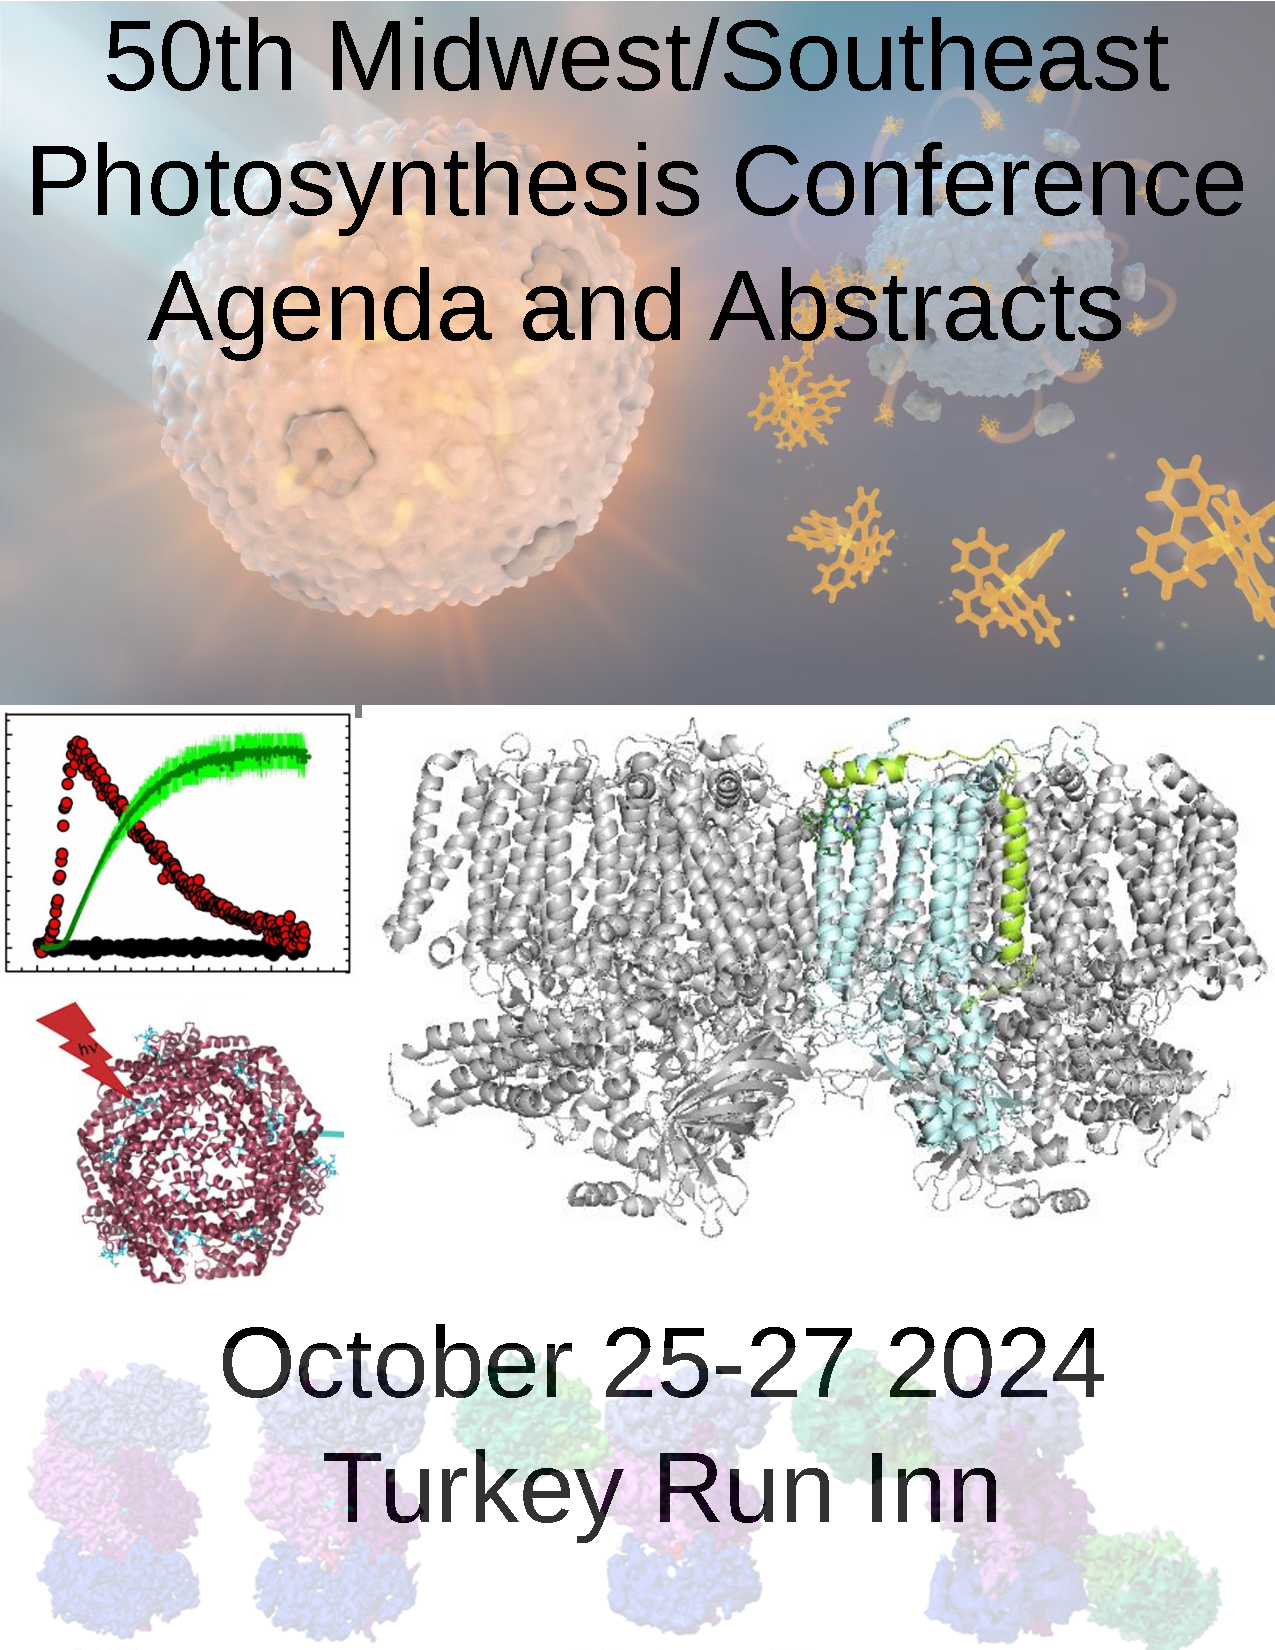
\includepdf{images/cover.pdf} % The cover for the booklet is included as a whole-page image, it can be a PDF or an image file but must be the same dimensions as the paper size

%----------------------------------------------------------------------------------------
%	 INFORMATION/COPYRIGHT PAGE
%----------------------------------------------------------------------------------------

\thispagestyle{empty} % Suppress headers and footers on this page

%~\vfill % Push text down
%
%\begin{center}	
%	This is the short version of the booklet for print use. \\ Full abstracts with all authors, references, and figures can be found at:\\ \url{https://amcosconference.com/}
%	
%	This template originates from \url{LaTeXTemplates.com} and is based on the original version at:\\ \url{https://github.com/maximelucas/AMCOS\_booklet}
%\end{center}
%
%\newpage

%----------------------------------------------------------------------------------------
%	 TABLE OF CONTENTS
%----------------------------------------------------------------------------------------

\tableofcontents

%----------------------------------------------------------------------------------------
%	 ABOUT CONFERENCE
%----------------------------------------------------------------------------------------



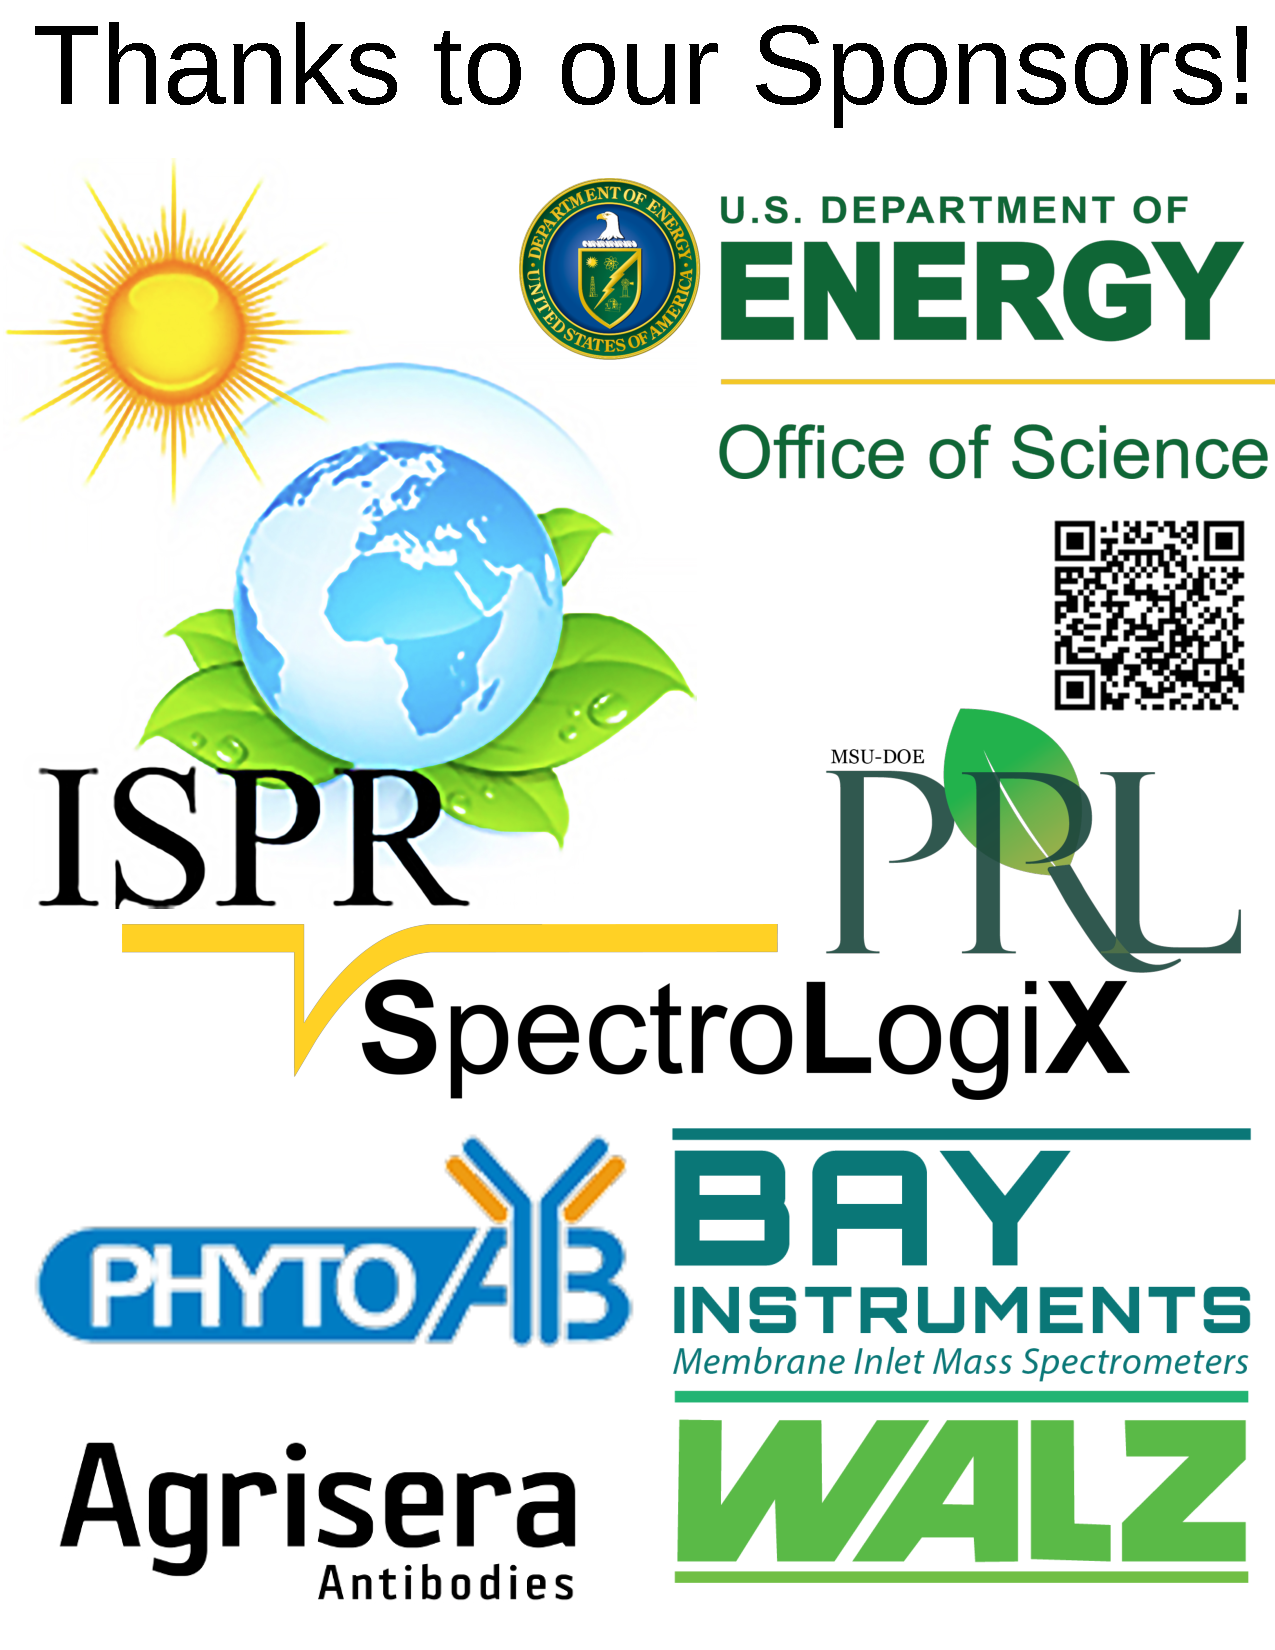
\includepdf[addtotoc={1,chapter,0,Sponsors,sponsors}]{images/sponsors.pdf}

%----------------------------------------------------------------------------------------
%	 TIMETABLE
%----------------------------------------------------------------------------------------

\chapter{Program}

%CT: Contributed Talk, IS: Invited Speaker, KL: Keynote Lecture, IT: Invited Talk.
\vspace{-24pt}
\section{Friday, October 25}

\begin{longtable}{|C{0.15\linewidth}| C{0.1\linewidth}|  C{0.3\linewidth} C{0.0\linewidth} C{0.4\linewidth}|}\hline	
	\eventtype{4:00--6:00pm}{Registration and Poster Hanging}
	\tablebreak{6:00pm}{Dinner}
	\eventtype{7:30--7:40pm}{Introduction and Welcome}
	\KL{7:40--8:20pm}{Govindjee}{University of Illinois at Urbana-Champaign}{Photosynthesis: stories from the past}
	\CT{8:20--8:40pm}{Chris Gisriel}{University of Wisconsin}{\hyperlink{Gisriel.1}{Structure and evolution of Photosystem I in the early-branching cyanobacterium \emph{Anthocerotibacter panamensis}}}
	\CT{8:40--9:00pm}{Nina Ponomarenko}{Argonne National Laboratory}{\hyperlink{Ponomarenko.1}{Structural Analysis of Platinum Nanoclusters Assembled on Photosystem I by Light-Driven Chemistry}}
	\CT{9:00--9:20pm}{Rajnandani Kashyap}{St. Louis University School of Medicine}{\hyperlink{Kashyap.1}{Cryo-EM reveals a bi-copper cluster coordinating asymmetric electron transfer in the nitrogenase-like DPOR complex}}
	\eventtype{9:30pm}{Mixer and Poster Session}
\end{longtable}

%------------------------------------------------

\section{Saturday, October 26}

\begin{longtable}{|C{0.15\linewidth}| C{0.1\linewidth}|  C{0.3\linewidth} C{0.0\linewidth} C{0.4\linewidth}|}\hline	
	\tablebreak{7:00am}{Breakfast}
	\KL{9:00--9:40am}{Lauren Ann Metskas}{Purdue University}{Rubisco polymerization inside alpha-carboxysomes - but how and why?}
	\CT{9:40--10:00am}{Rees Rillema}{Michigan State University}{\hyperlink{Rillema.1}{Gas exchanges measurements of carboxysome mutants reveal conditional phenotypes and insights into cyanobacteria carbon concentrating mechanism}}
	\CT{10:00--10:20am}{Chetna Sharma}{ University of Florida}{\hyperlink{Sharma.1}{KDPG aldolase modulates the photosynthetic carbon yield in Synechococcus elongatus PCC 7942}}
	\tablebreak{10:20--10:40am}{Coffee}
	\CT{10:40--11:00am}{Alize\'e Malno\"e}{Indiana University Bloomington}{\hyperlink{Malnoe.1}{qH-energy dissipation in photosystem II antennae}}
	\CT{11:00--11:20am}{Grant Steiner}{Loyola University Chicago}{\hyperlink{Steiner.1}{Extreme light acclimation reveals inherent photosystem II photoprotection in a natively low-light \emph{Chlorella}}}
	\CT{11:20--11:40am}{Amala Phadkule}{Purdue University}{\hyperlink{Phadkule.1}{Tuning the low-energy fluorescence state in photosystem II}}
	\CT{11:40--12:00pm}{Mohamed Elrefaiy}{The University of Texas at Austin}{\hyperlink{Elrefaiy.1}{Computational prediction and experimental validation of pKa shifts in the Q57D mutant of \emph{Lepidium virginicum} WSCP: implications for 
		tailored chlorophyll protein design	}}
	\CT{12:00--12:20pm}{Jasleen Bindra}{Argonne National Laboratory}{
		\hyperlink{Bindra.1}{Coherences of photo-induced electron spin qubit pair states in natural photosynthetic proteins}
	}
	\tablebreak{12:30pm}{Lunch}
	\eventtype{Afternoon}{Free to explore Turkey Run State Park}
	\eventtype{4:00--6:00pm}{Poster Session}
	\tablebreak{6:00pm}{Dinner}
	\KL{7:30--8:10pm}{David Vinyard}{Louisiana State University}{\hyperlink{Vinyard.1}{A Photosynthetic Variant of \emph{Synechocystis} sp. PCC 6803 Sacrifices a Stress Response Pathway to Outcompete its Peers under Optimal Growth Conditions
	}}
	\CT{8:10--8:30pm}{K. V. Lakshmi}{Rensselaer Polytechnic Institute, New York}{\hyperlink{Lakshmi.1}{Understanding the mechanism of substrate delivery and binding in the oxygen-evolving complex of photosystem II}}
	\IS{8:30--8:40pm}{Colin Gates}{Loyola University Chicago}{Remembering Jeffery Cameron}
	\IS{8:40--8:50pm}{Chris Gisriel}{University of Wisconsin}{Remembering Donald Bryant}
	\eventtype{9:00pm}{50th Anniversary Cake, Campfire, Drinks, and Poster Session }

	
\end{longtable}

%------------------------------------------------

\section{Sunday, October 27}


\begin{longtable}{|C{0.15\linewidth}| C{0.1\linewidth}|  C{0.3\linewidth} C{0.0\linewidth} C{0.4\linewidth}|}\hline	
	
	\tablebreak{7:00am}{Breakfast}
	\KL{9:00--9:40am}{Wim Vermaas}{Arizona State University}{\hyperlink{Vermaas.1}{50 years of cyanobacteria and photosynthesis}}
	\CT{9:40--10:00am}{Christopher Jones}{Washington University, St. Louis}{\hyperlink{Jones.1}{ACCESSing the carbon uptake dynamics of cyanobacteria}}
	\CT{10:00--10:20am}{Harvey Hou}{Alabama State University}{\hyperlink{Hou.1}{Tri-institutional effort to probe cyanobacterial metabolic overflow: 
		from research to training}
	}
	\CT{10:20--10:40am}{Ashraf Mohamed}{The University of Texas at Austin}{
		\hyperlink{Mohamed.1}{A computational framework for simulating protein organization in thylakoid membranes}
	}
	\tablebreak{10:40--11:00am}{Coffee}
	\eventtype{11:00am}{Awards Presentations}
\end{longtable}

%----------------------------------------------------------------------------------------
%	 LIST OF TALK ABSTRACTS
%----------------------------------------------------------------------------------------

% Abstract template
%\abstract
%	{} % Title
%	{} % Author(s)
%	{} % Tag, can be: empty, \KLtag (keynote lecture), \IStag (invited speaker), \CTtag (contributed talk) or \ITtag (invited talk)
%	{} % Affiliation(s)
%	{} % Abstract text

\chapter{Talk Abstracts}
\begin{itemize}
	\item \hyperlink{Bindra.1}{Bindra} pg. \pageref{abs:Bindra}
\item \hyperlink{Elrefaiy.1}{Elrefaiy} pg. \pageref{abs:Elrefaiy}
\item \hyperlink{Gisriel.1}{Gisriel} pg. \pageref{abs:Gisriel}
\item \hyperlink{Hou.1}{Hou} pg. \pageref{abs:Hou}
\item \hyperlink{Jones.1}{Jones} pg. \pageref{abs:Jones}
\item \hyperlink{Kashyap.1}{Kashyap} pg. \pageref{abs:Kashyap}
\item \hyperlink{Lakshmi.1}{Lakshmi} pg. \pageref{abs:Lakshmi}
\item \hyperlink{Malnoe.1}{Malnoe} pg. \pageref{abs:Malnoe}
\item \hyperlink{Metskas.1}{Metskas} pg. \pageref{abs:Metskas}
\item \hyperlink{Mohamed.1}{Mohamed} pg. \pageref{abs:Mohamed}
\item \hyperlink{Phadkule.1}{Phadkule} pg. \pageref{abs:Phadkule}
\item \hyperlink{Ponomarenko.1}{Ponomarenko} pg. \pageref{abs:Ponomarenko}
\item \hyperlink{Rillema.1}{Rillema} pg. \pageref{abs:Rillema}
\item \hyperlink{Sharma.1}{Sharma} pg. \pageref{abs:Sharma}
\item \hyperlink{Steiner.1}{Steiner} pg. \pageref{abs:Steiner}
\item \hyperlink{Vermaas.1}{Vermaas} pg. \pageref{abs:Vermaas}
\item \hyperlink{Vinyard.1}{Vinyard} pg. \pageref{abs:Vinyard}

\end{itemize}
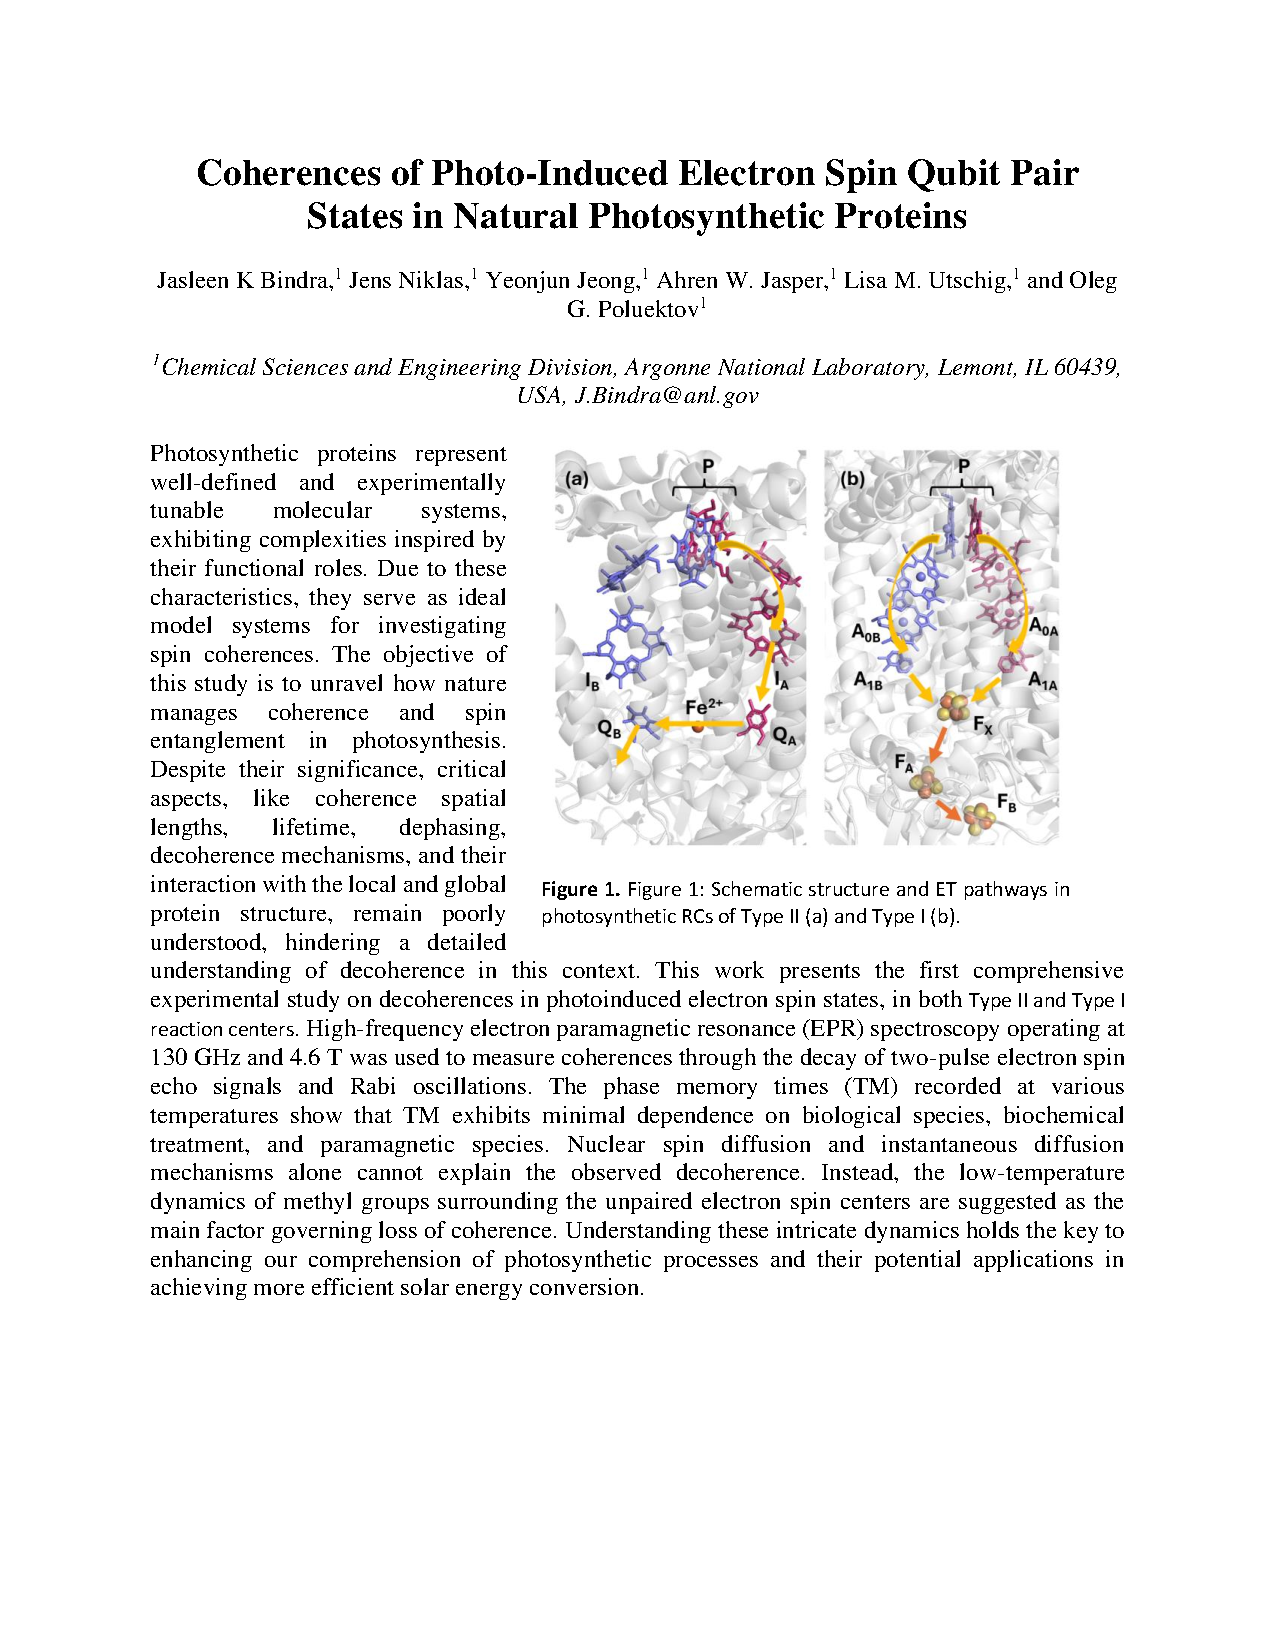
\includepdf[link=true,linkname=Bindra,pagecommand={\thispagestyle{plain}},addtolist={1,talk,heading,abs:Bindra}]{abstracts/Bindra_MWSE50.doc.pdf}
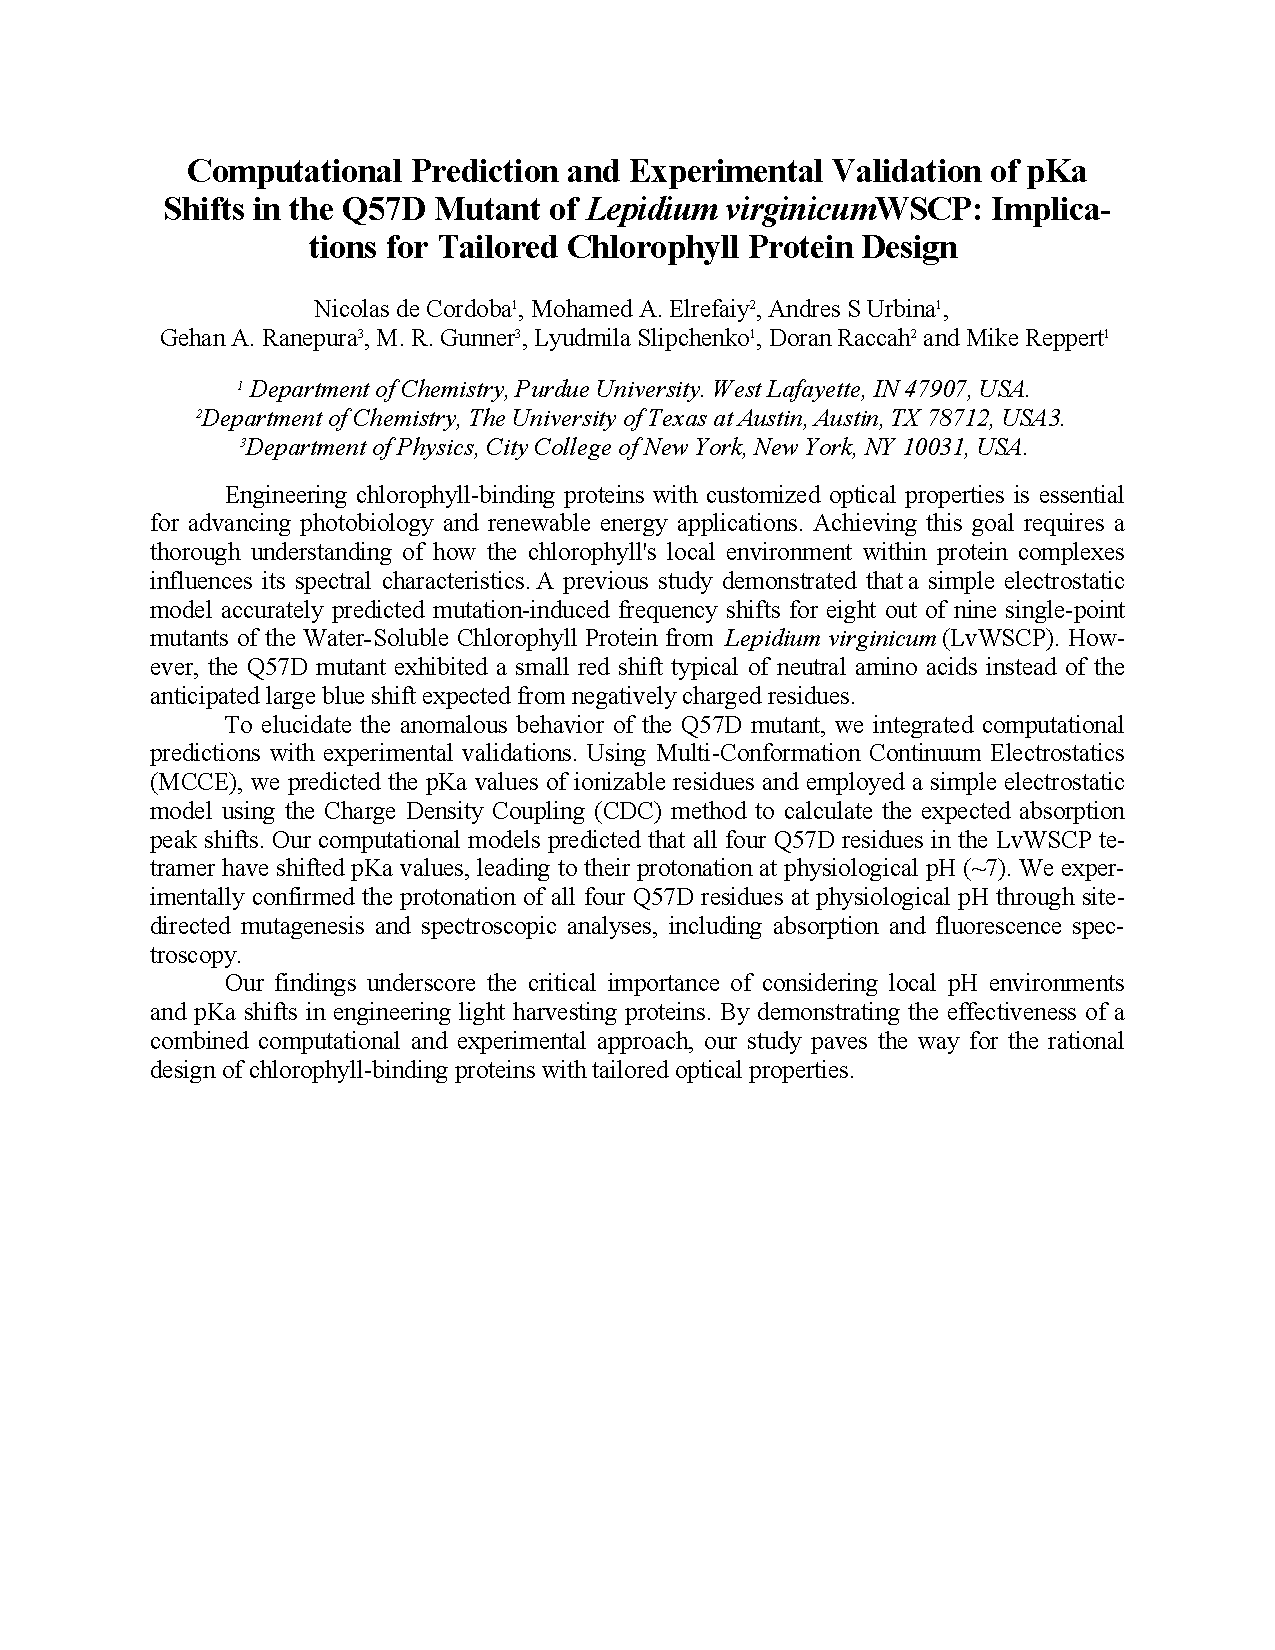
\includepdf[link=true,linkname=Elrefaiy,pagecommand={\thispagestyle{plain}},addtolist={1,talk,heading,abs:Elrefaiy}]{abstracts/Elrefaiy_MWSE50.pdf}
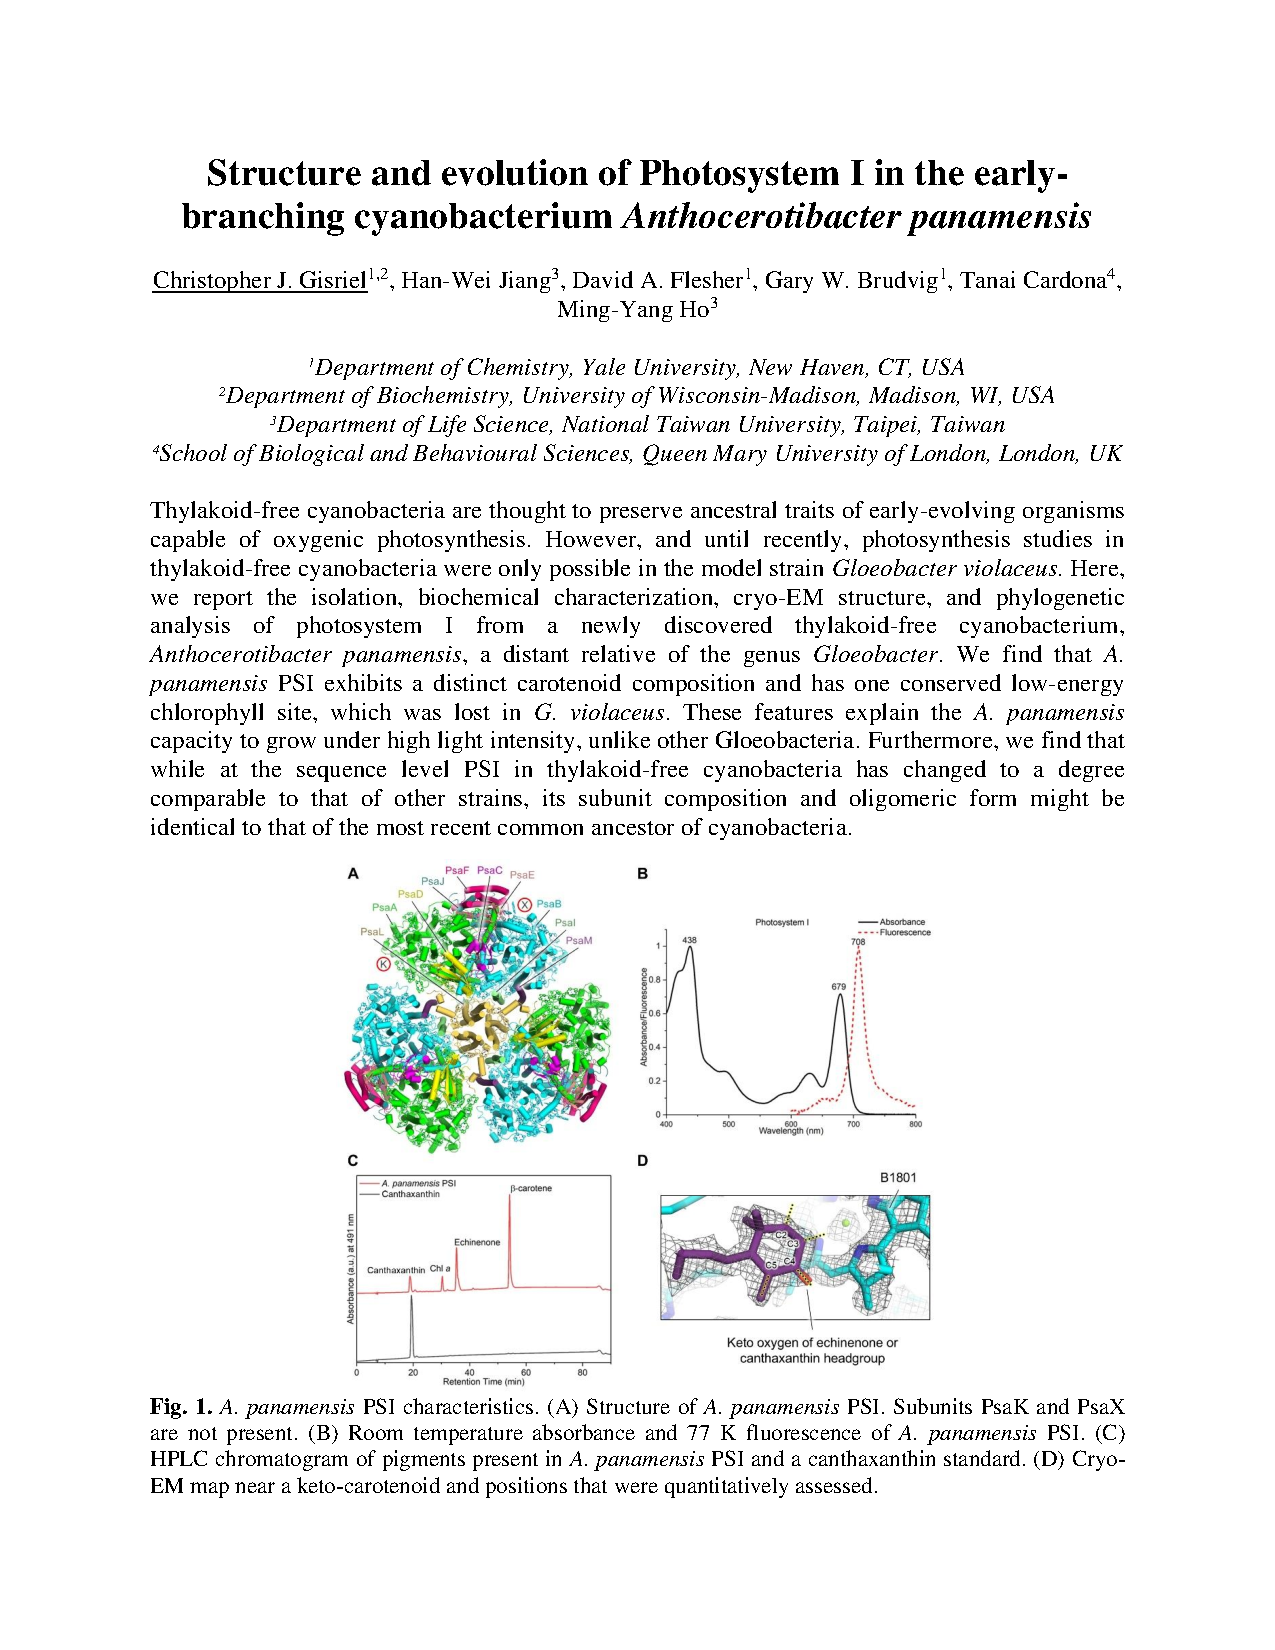
\includepdf[link=true,linkname=Gisriel,pagecommand={\thispagestyle{plain}},addtolist={1,talk,heading,abs:Gisriel}]{abstracts/Gisriel_MWSE50.pdf}
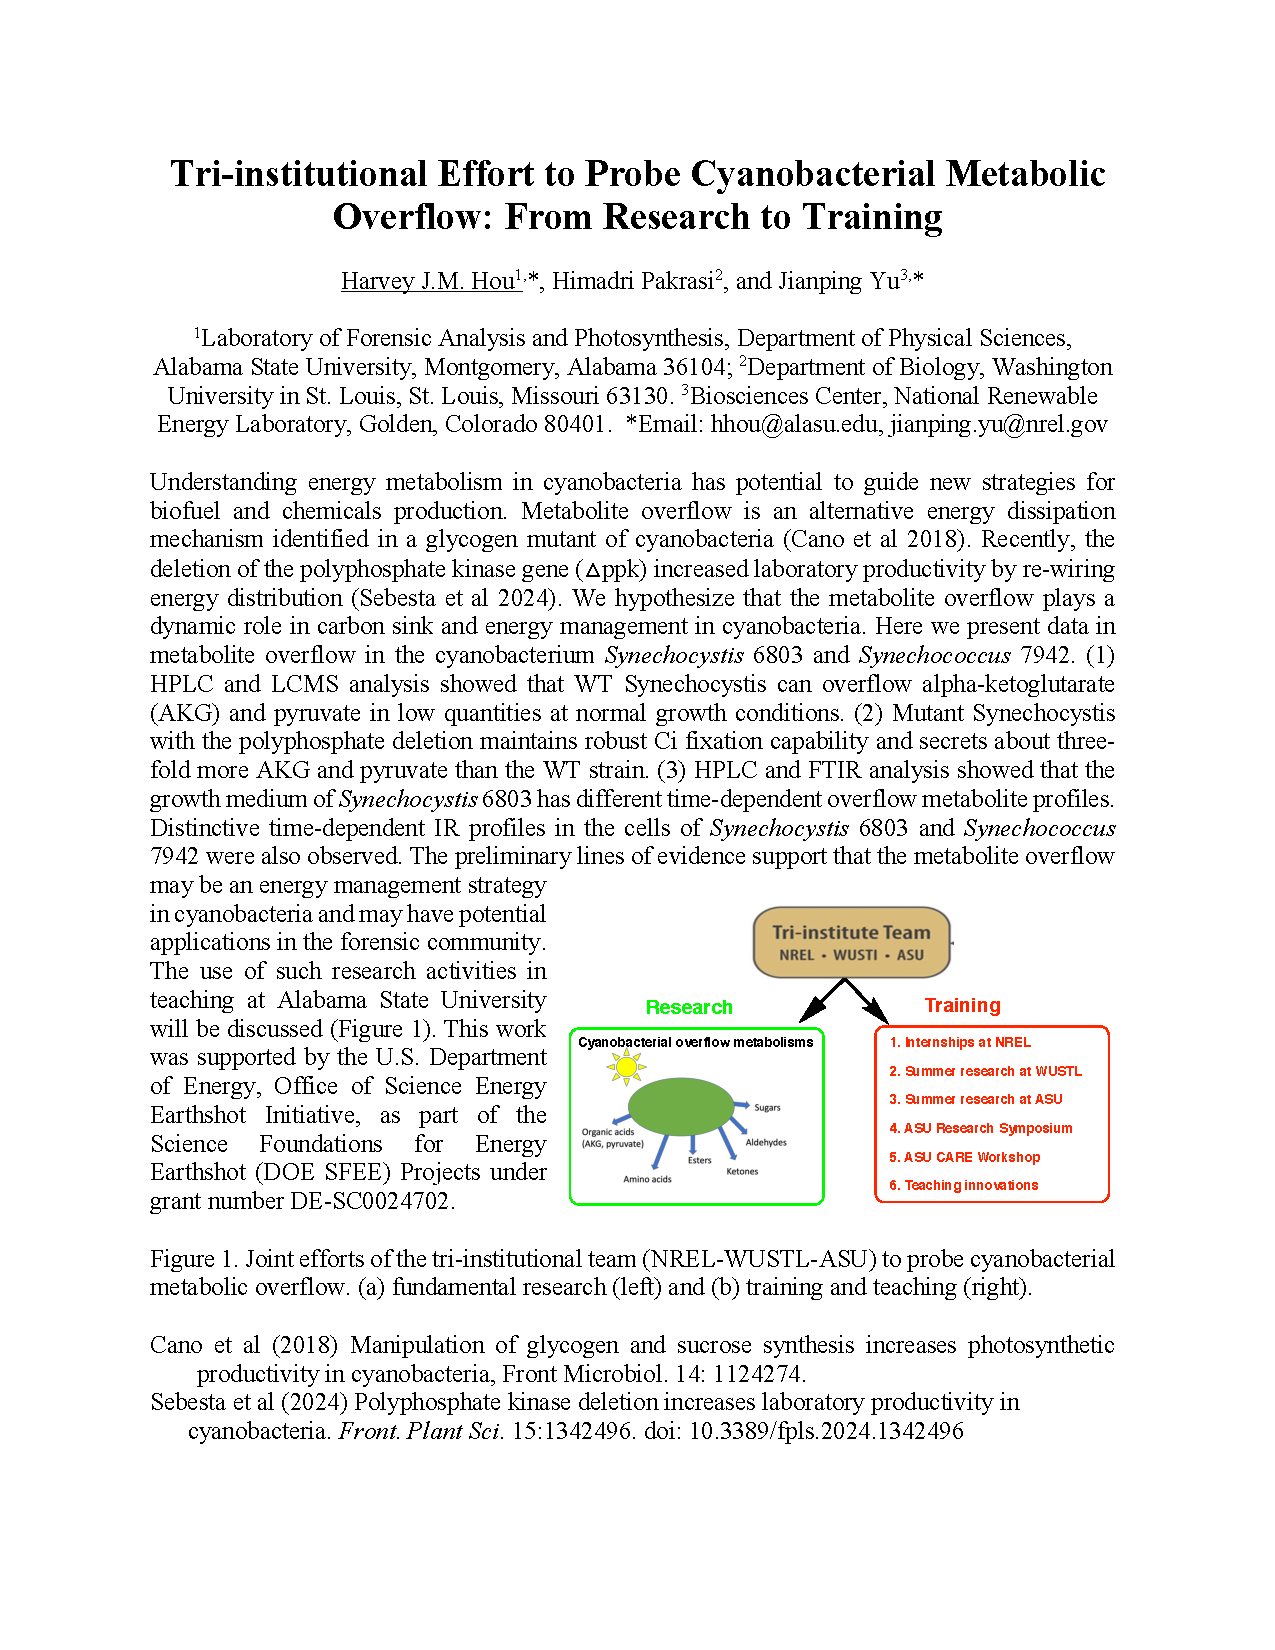
\includepdf[link=true,linkname=Hou,pagecommand={\thispagestyle{plain}},addtolist={1,talk,heading,abs:Hou}]{abstracts/hou_MWSE50.pdf}
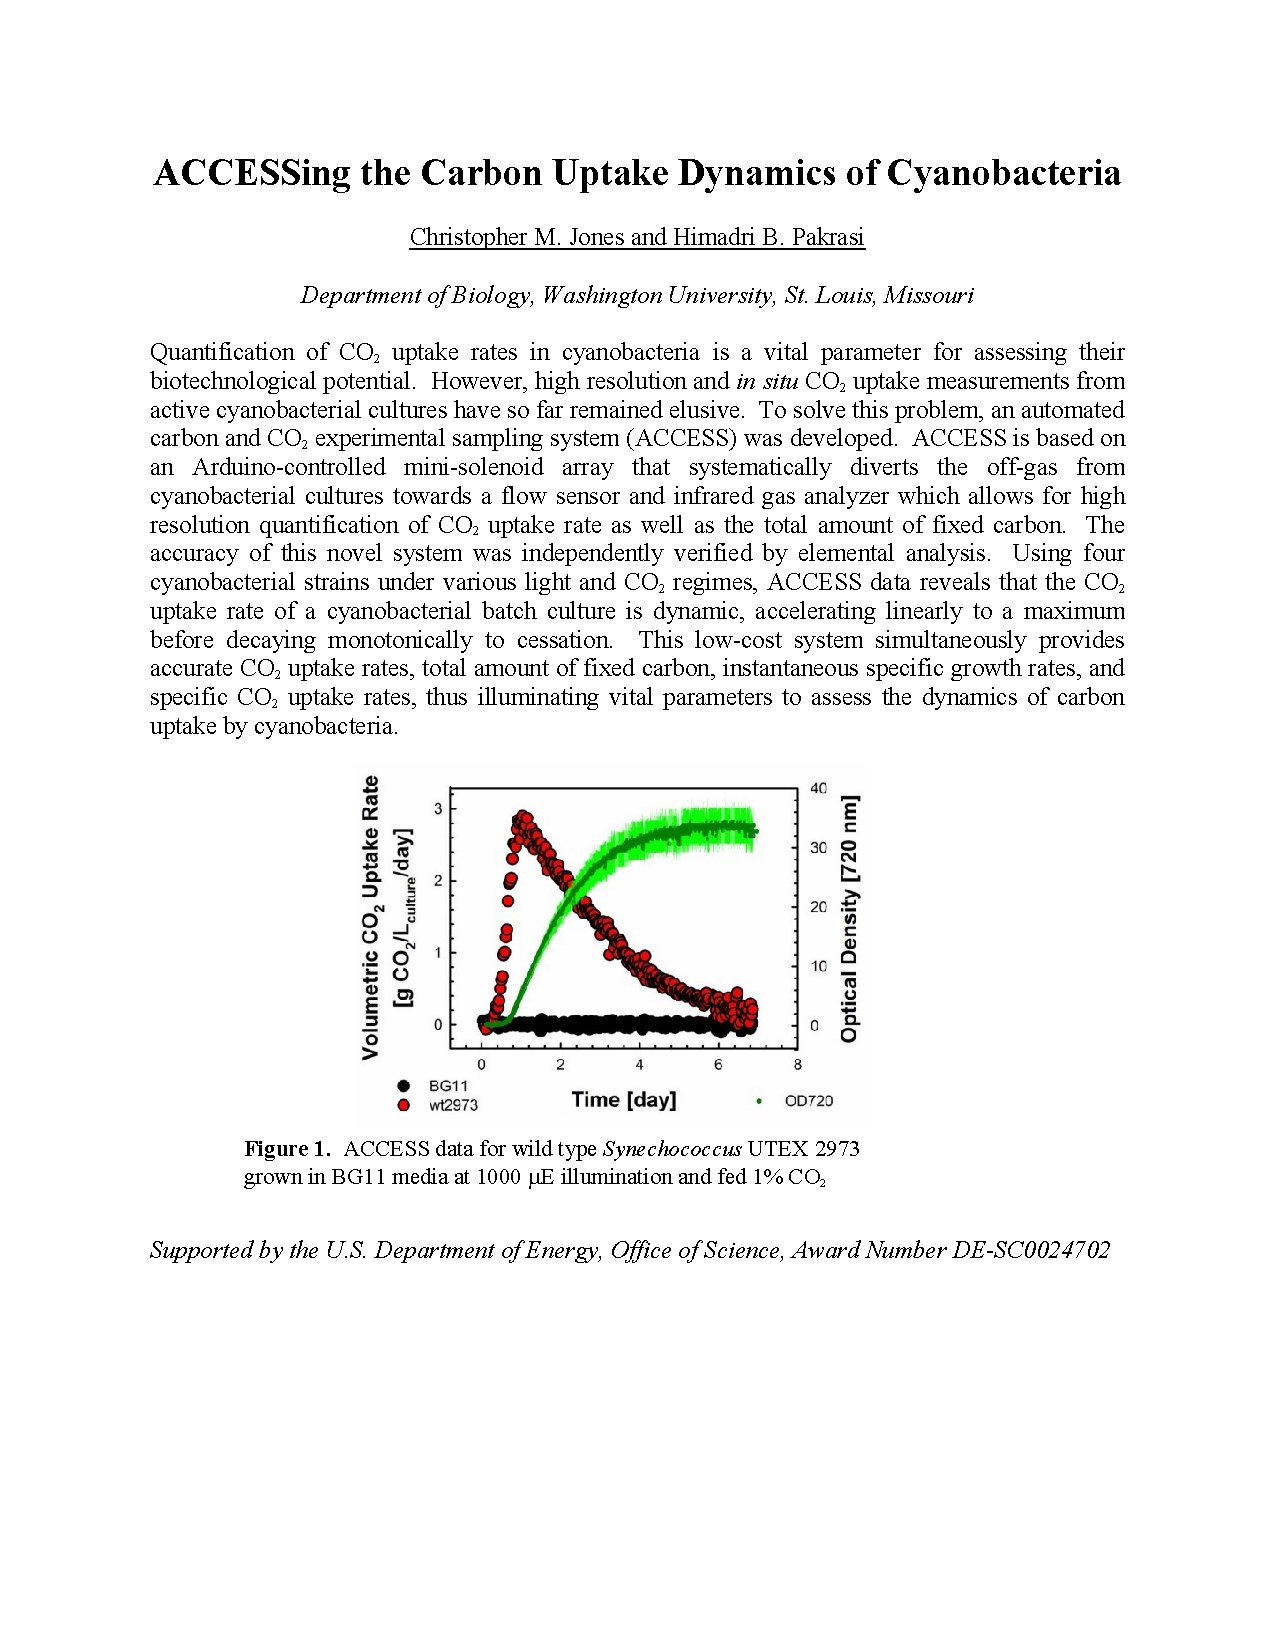
\includepdf[link=true,linkname=Jones,pagecommand={\thispagestyle{plain}},addtolist={1,talk,heading,abs:Jones}]{abstracts/Jones_MWSE50.pdf}
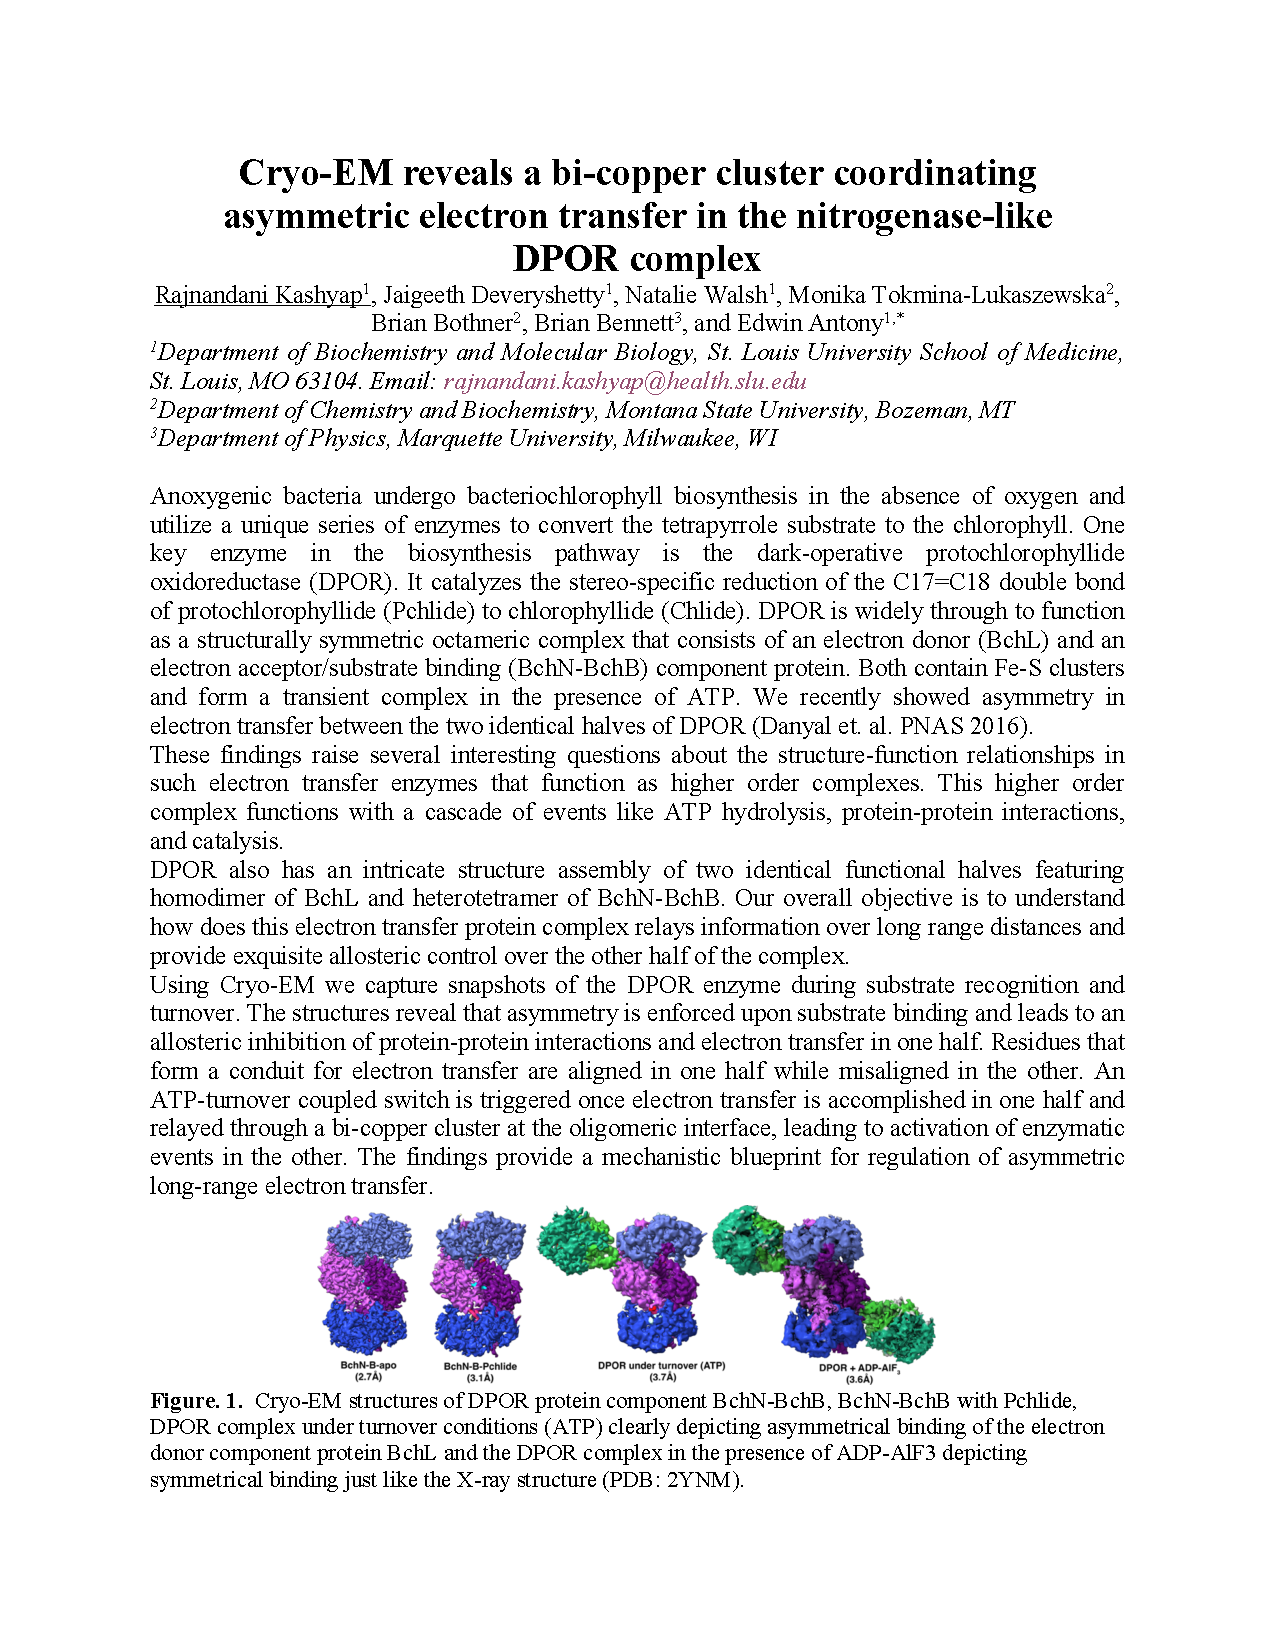
\includepdf[link=true,linkname=Kashyap,pagecommand={\thispagestyle{plain}},addtolist={1,talk,heading,abs:Kashyap}]{abstracts/Kashyap_MWSE50.pdf}
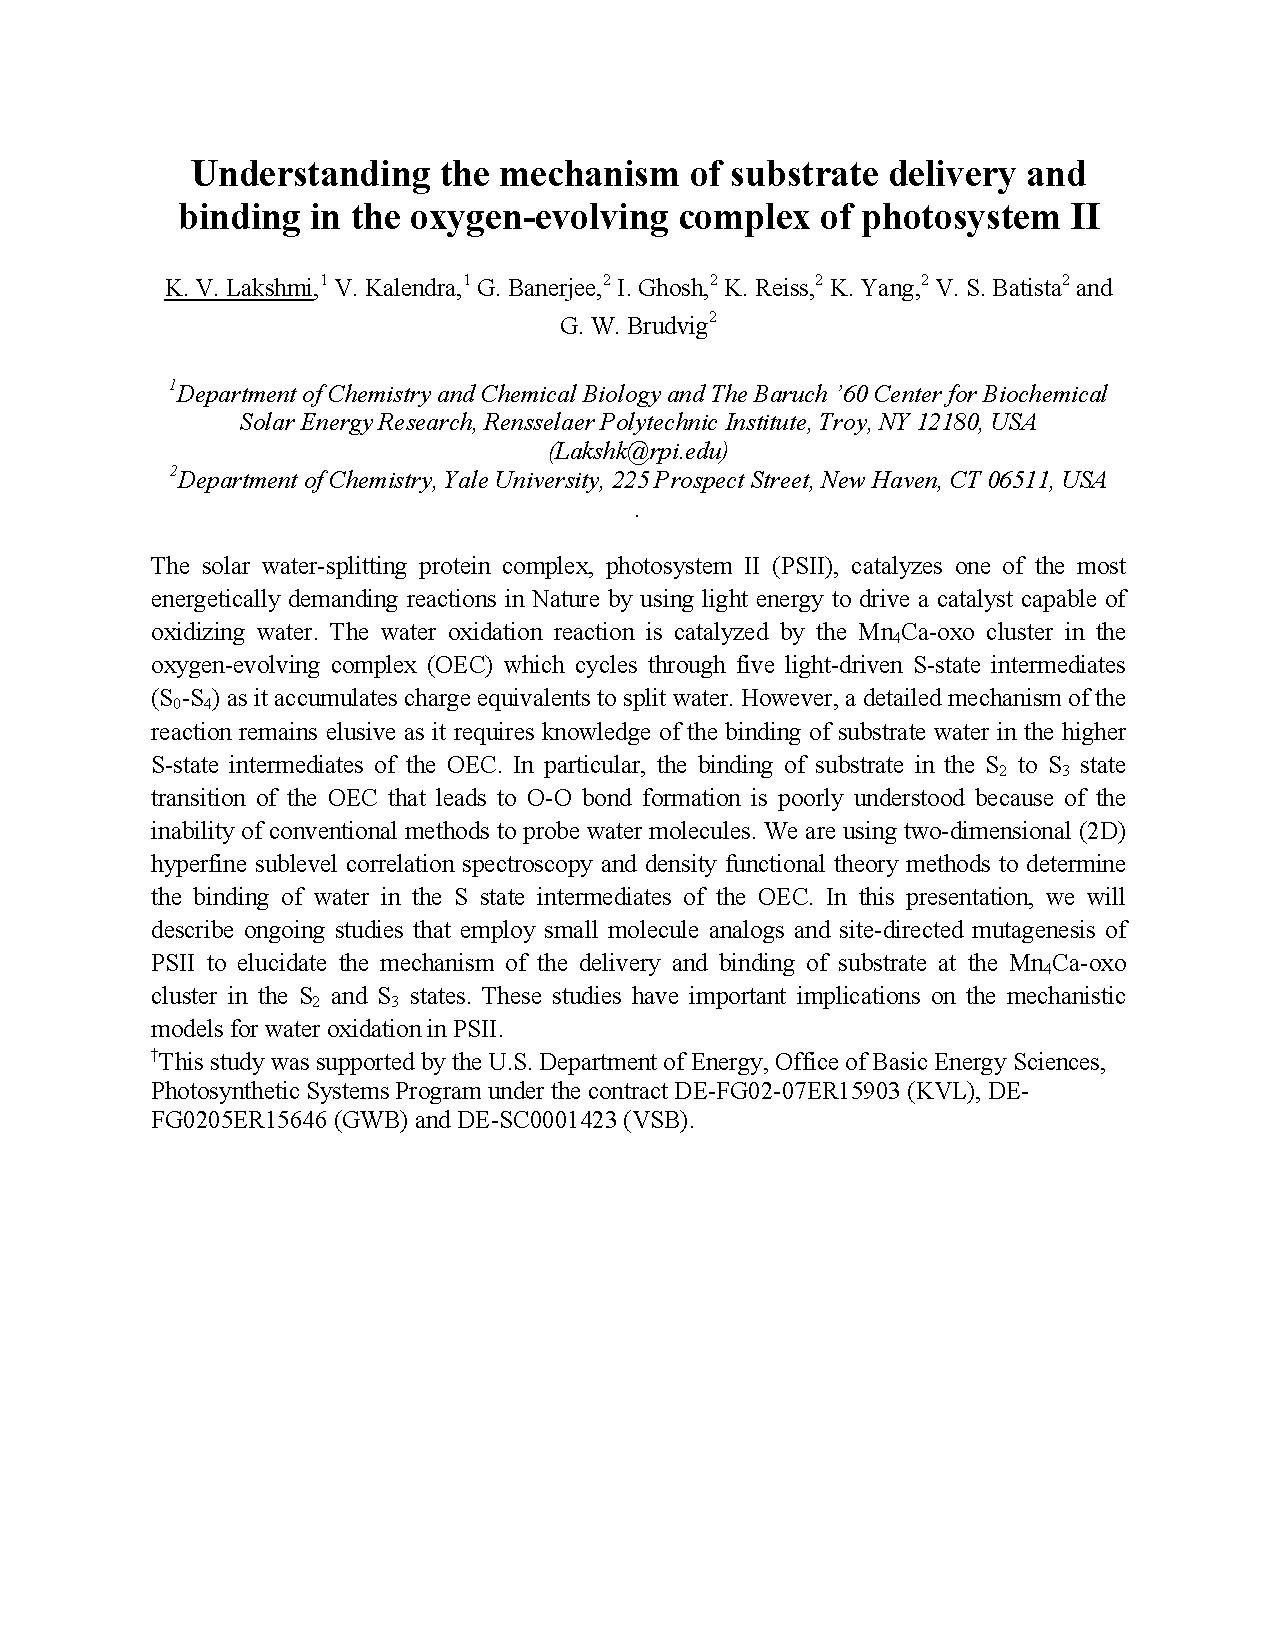
\includepdf[link=true,linkname=Lakshmi,pagecommand={\thispagestyle{plain}},addtolist={1,talk,heading,abs:Lakshmi}]{abstracts/Lakshmi_MWSE50.pdf}
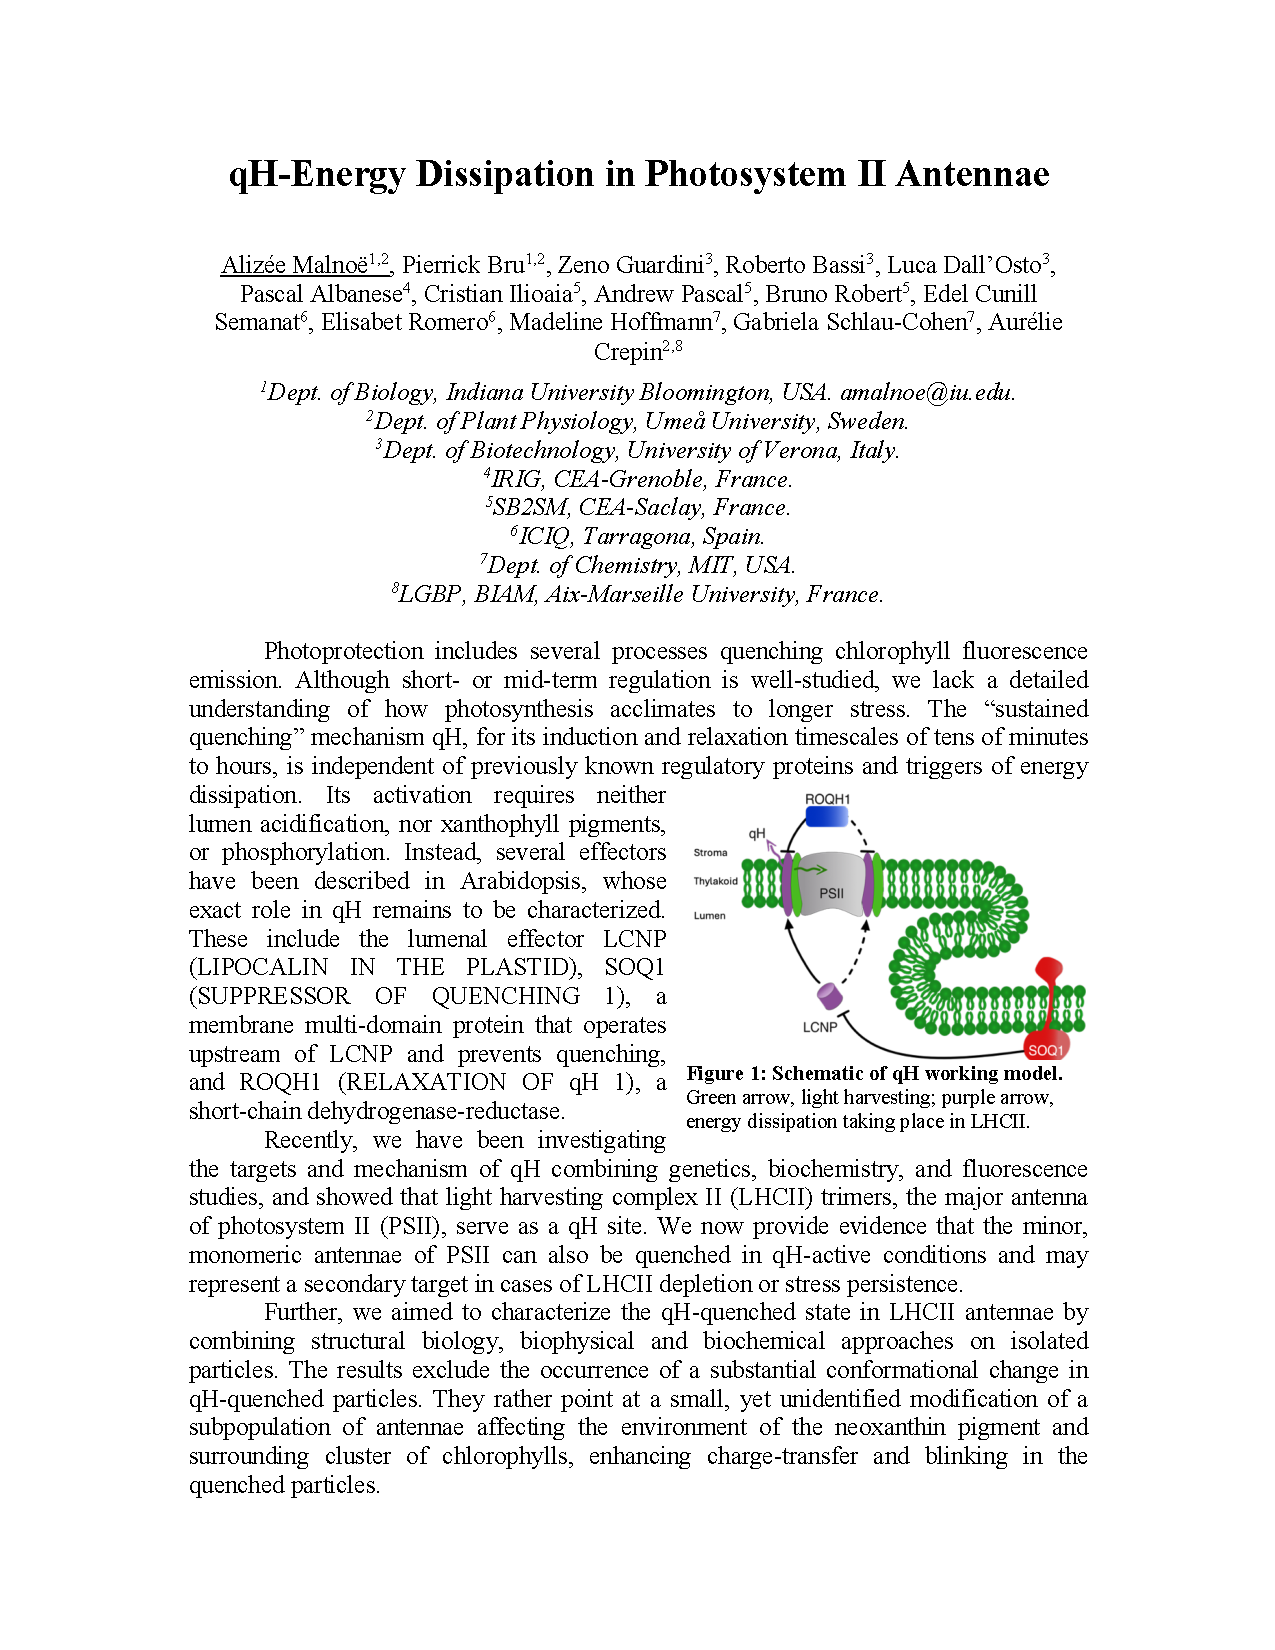
\includepdf[link=true,linkname=Malnoe,pagecommand={\thispagestyle{plain}},addtolist={1,talk,heading,abs:Malnoe}]{abstracts/Malnoe_MWSE50.pdf}
\includepdf[link=true,linkname=Metskas,pagecommand={\thispagestyle{plain}},addtolist={1,talk,heading,abs:Metskas}]{abstracts/Metskas_MWSE50.pdf}
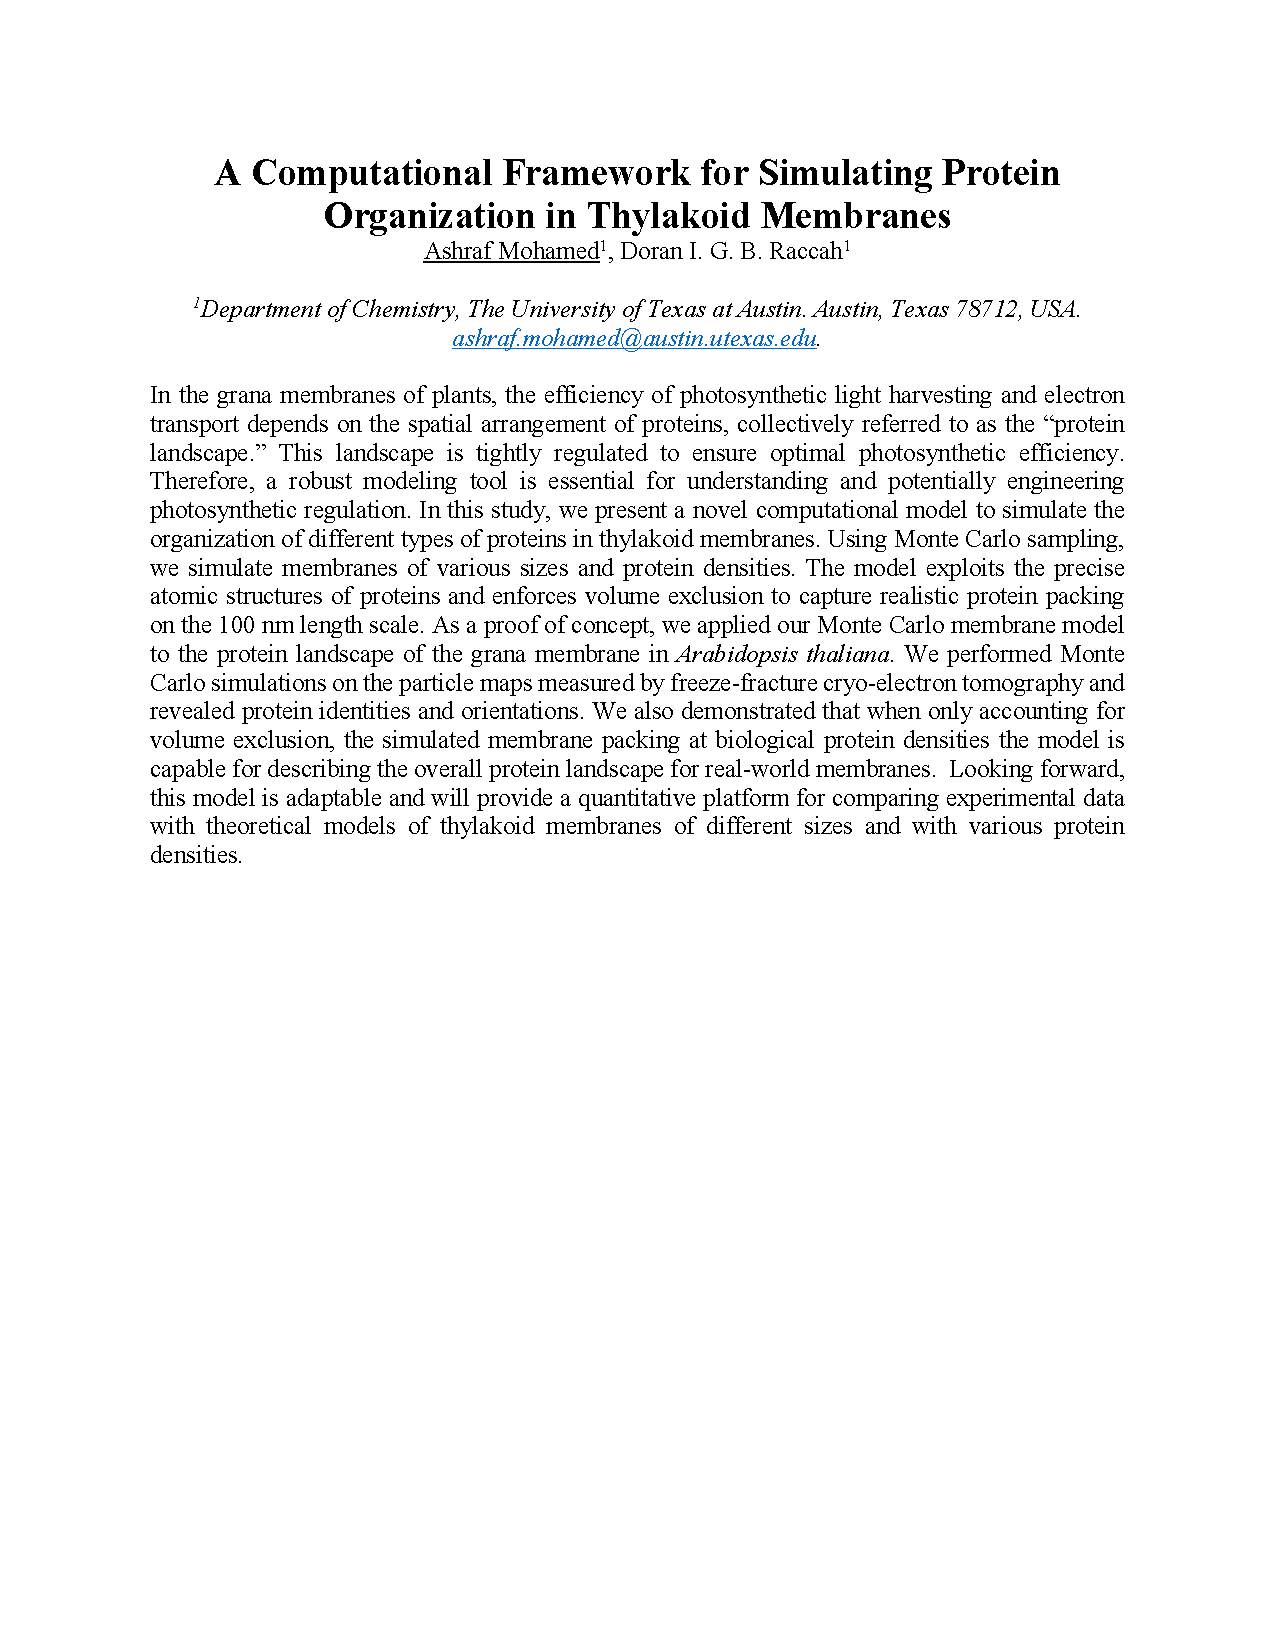
\includepdf[link=true,linkname=Mohamed,pagecommand={\thispagestyle{plain}},addtolist={1,talk,heading,abs:Mohamed}]{abstracts/Mohamed_MWSE50.pdf}
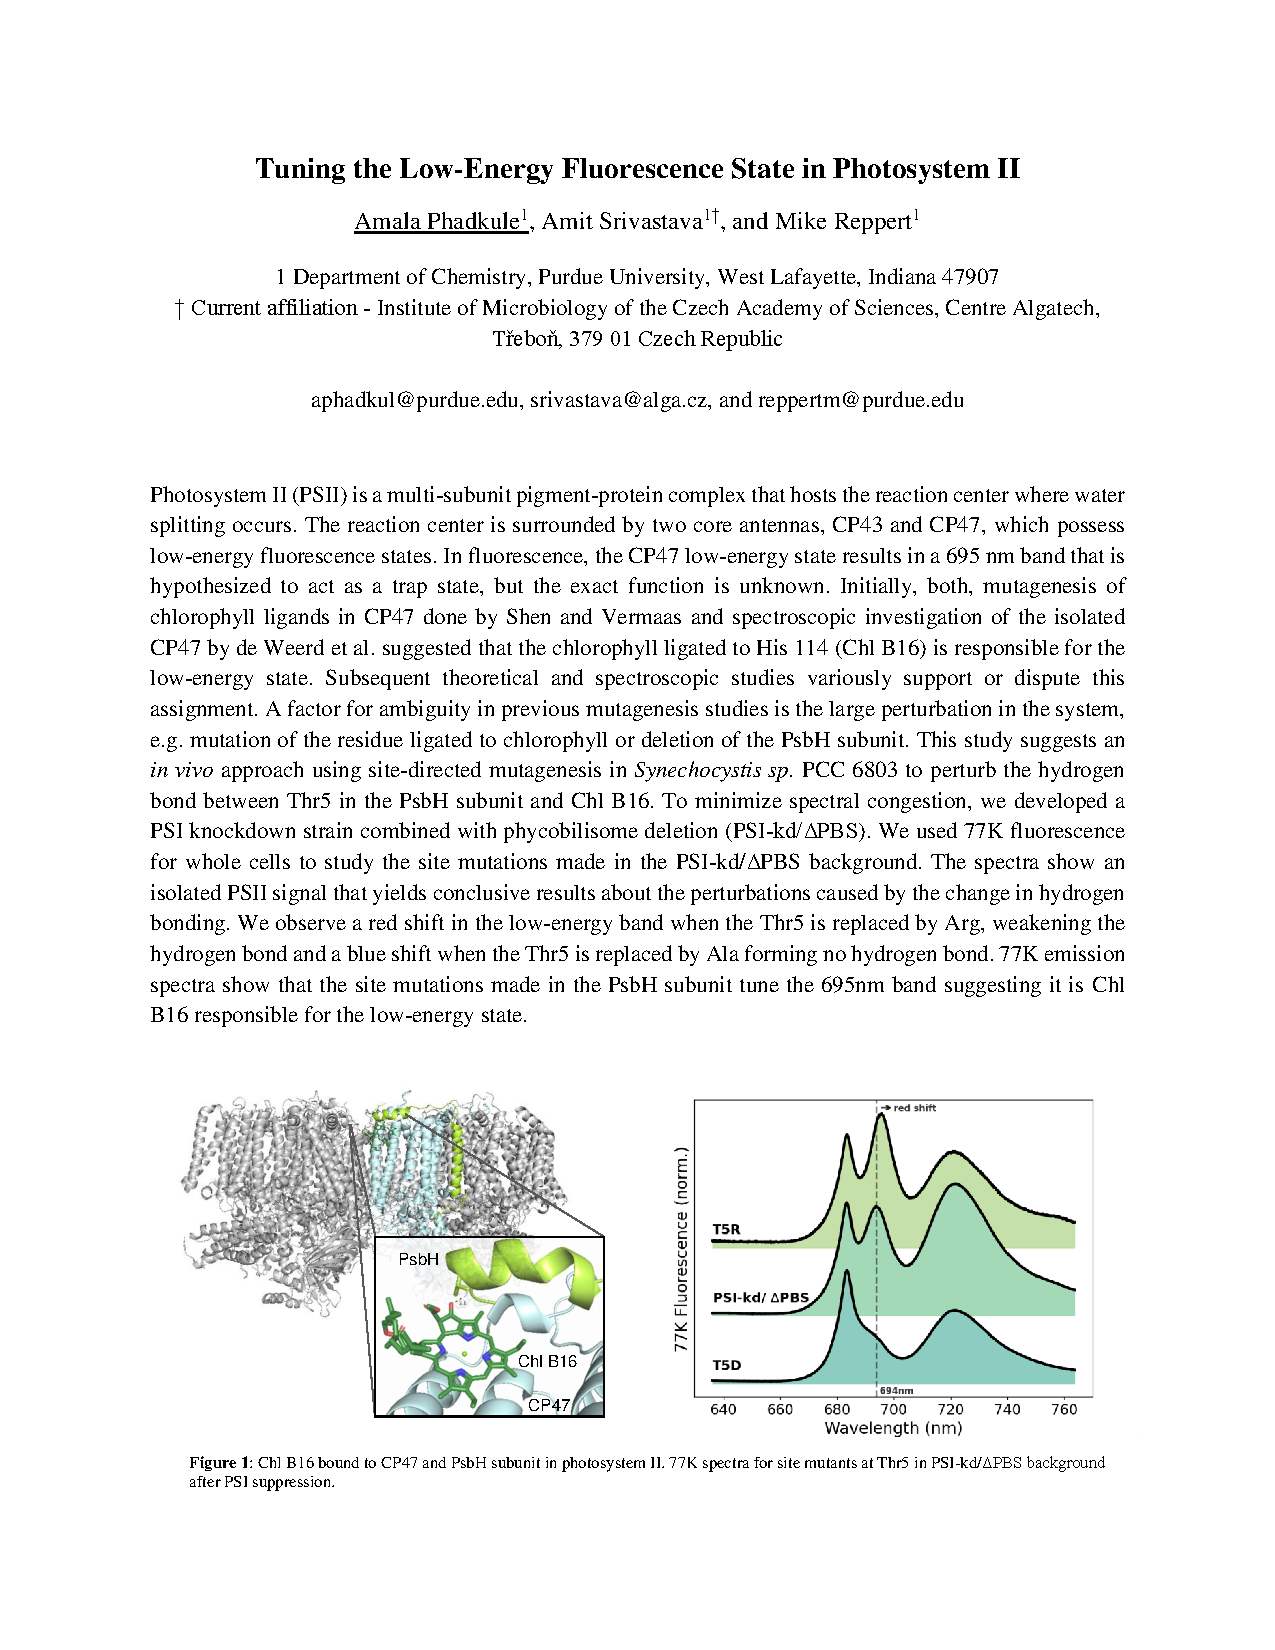
\includepdf[link=true,linkname=Phadkule,pagecommand={\thispagestyle{plain}},addtolist={1,talk,heading,abs:Phadkule}]{abstracts/Phadkule_MWSE50.pdf}
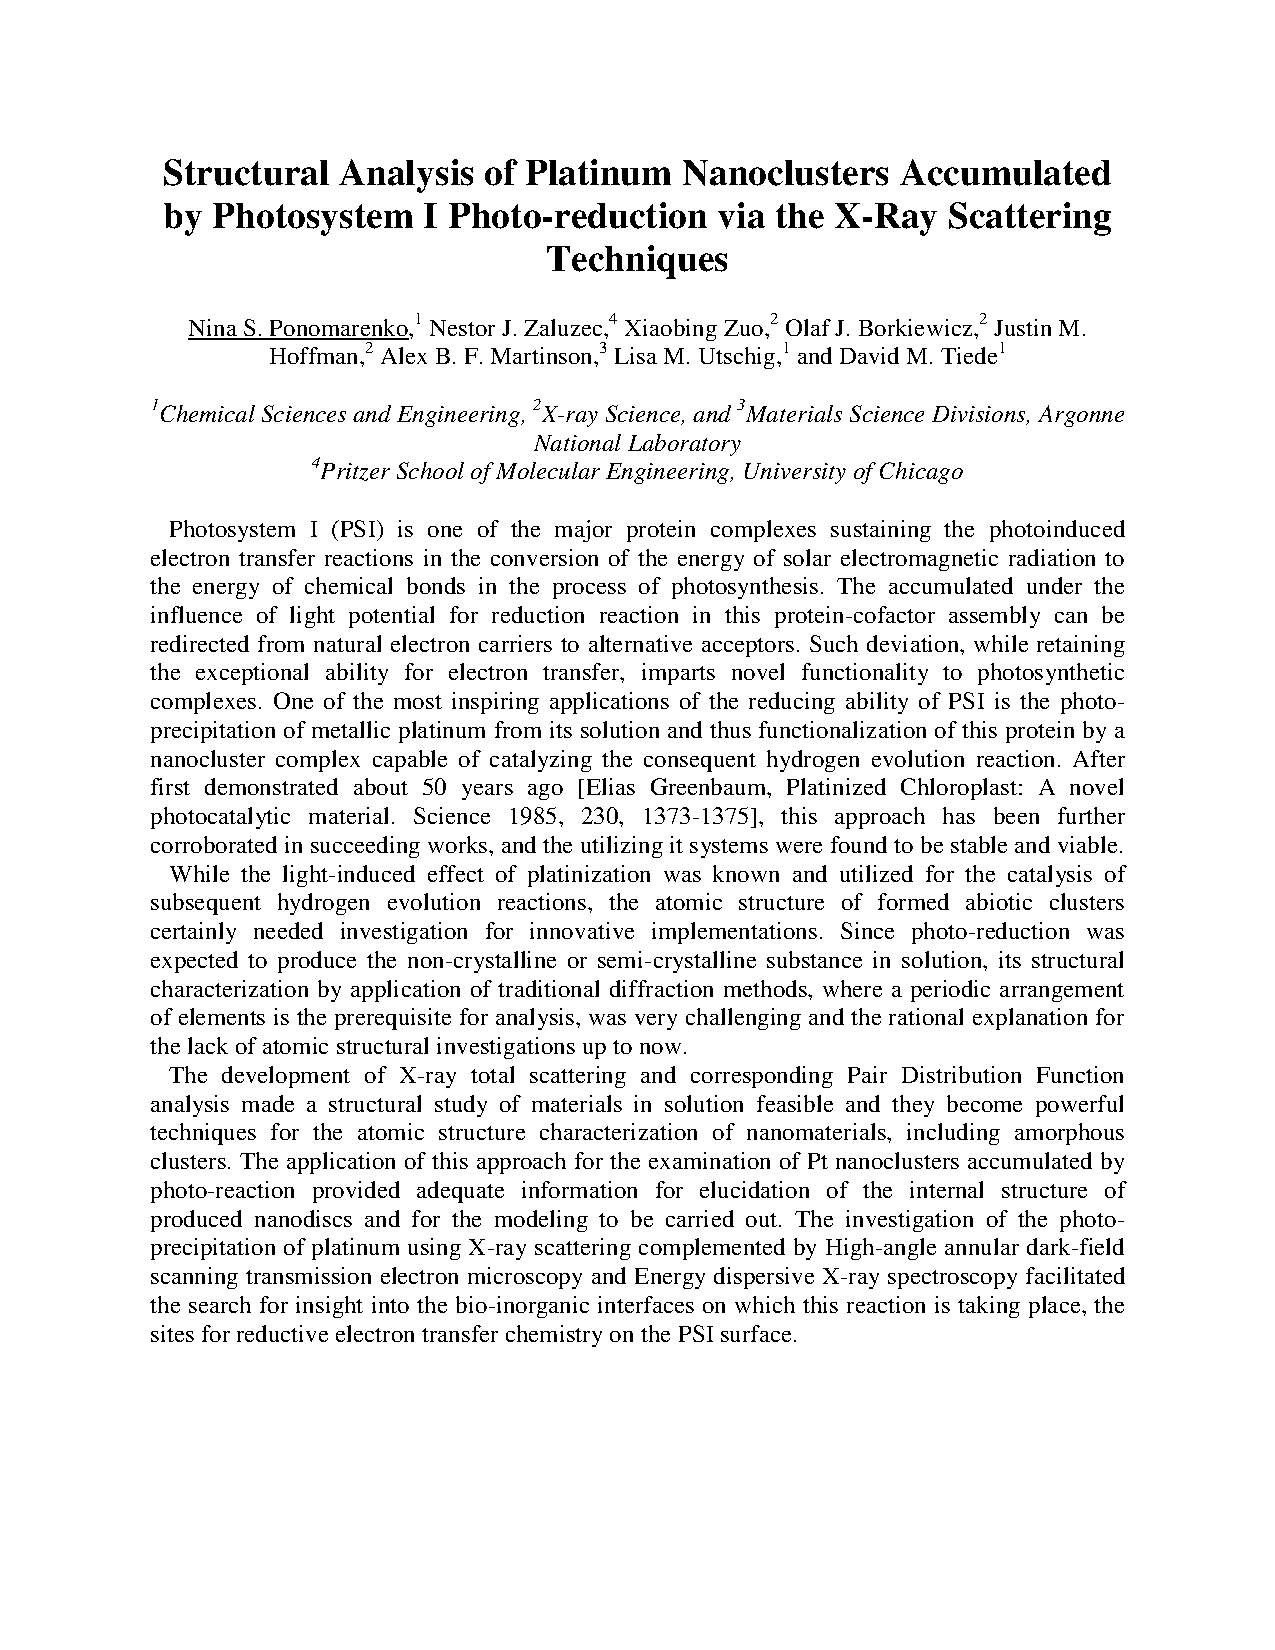
\includepdf[link=true,linkname=Ponomarenko,pagecommand={\thispagestyle{plain}},addtolist={1,talk,heading,abs:Ponomarenko}]{abstracts/Ponomarenko_MWSE50.pdf}
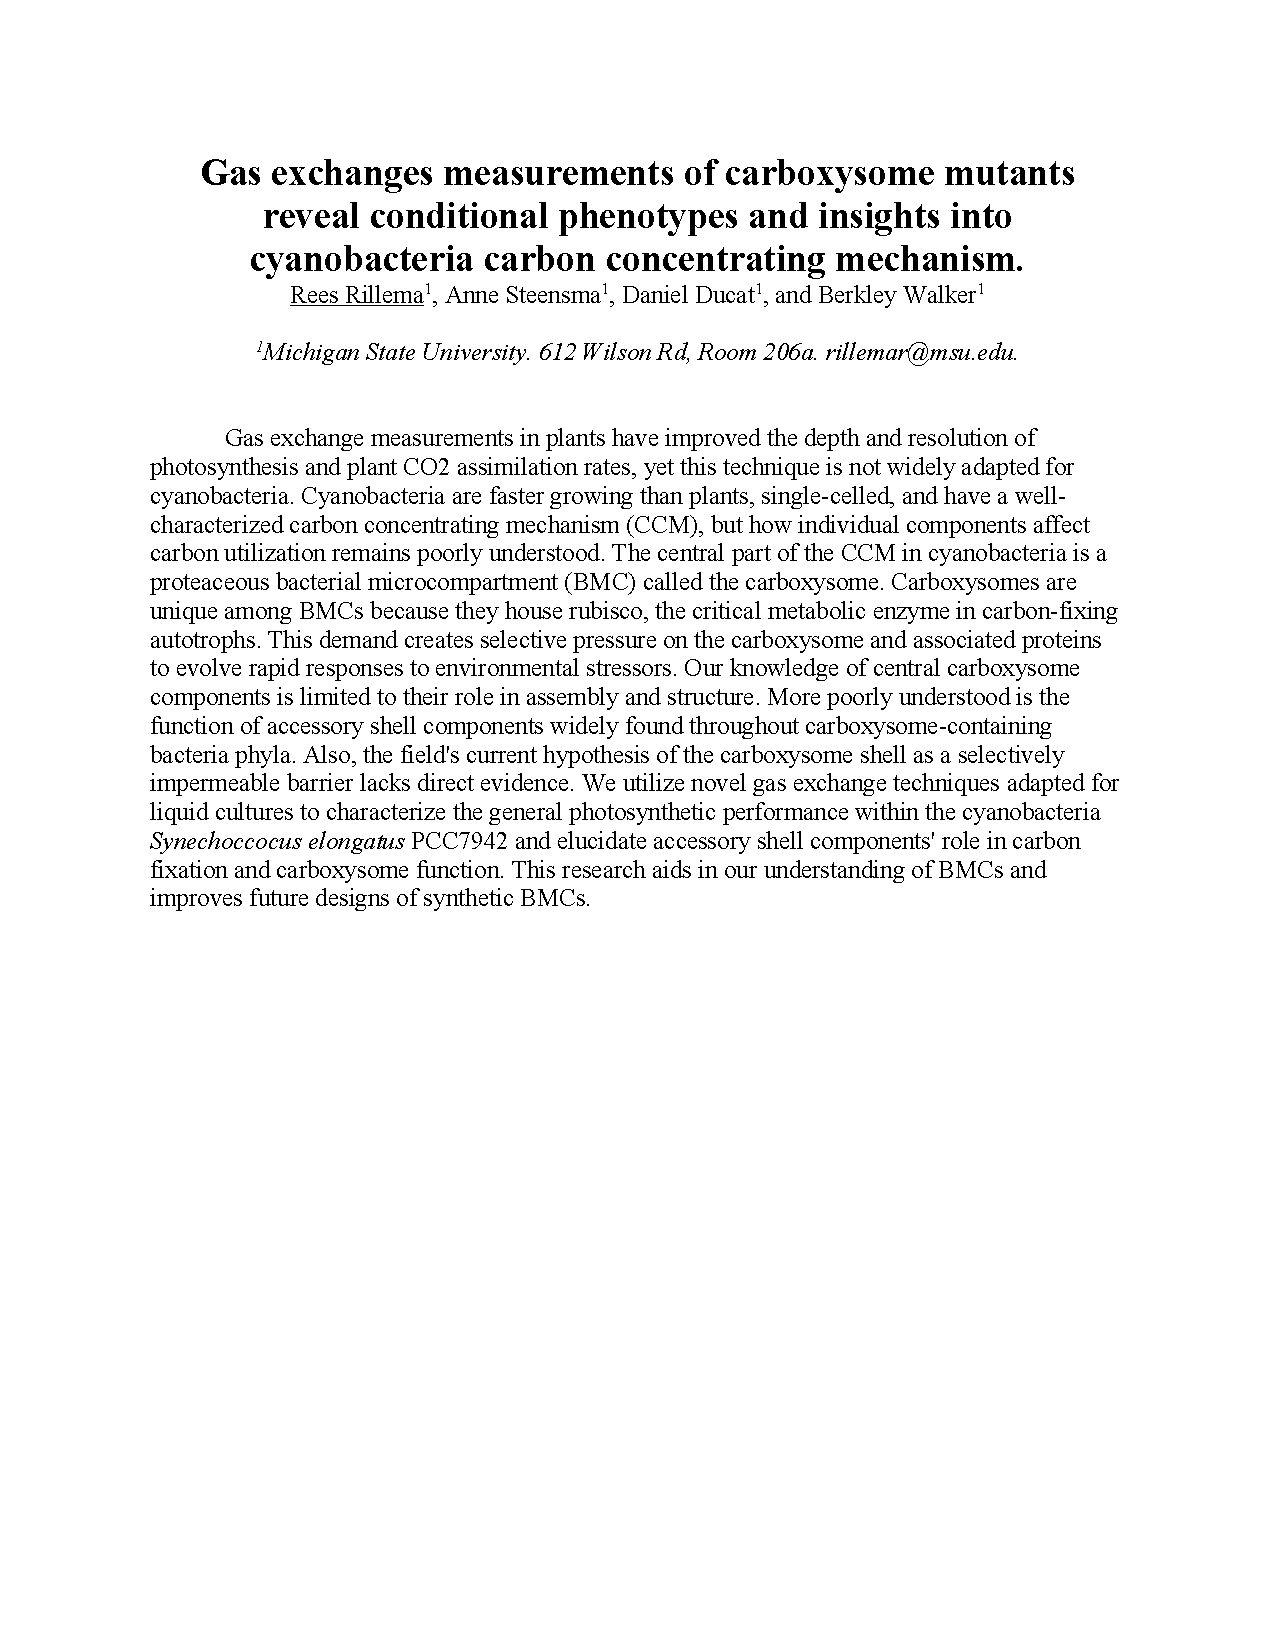
\includepdf[link=true,linkname=Rillema,pagecommand={\thispagestyle{plain}},addtolist={1,talk,heading,abs:Rillema}]{abstracts/Rillema_MWSE50.pdf}
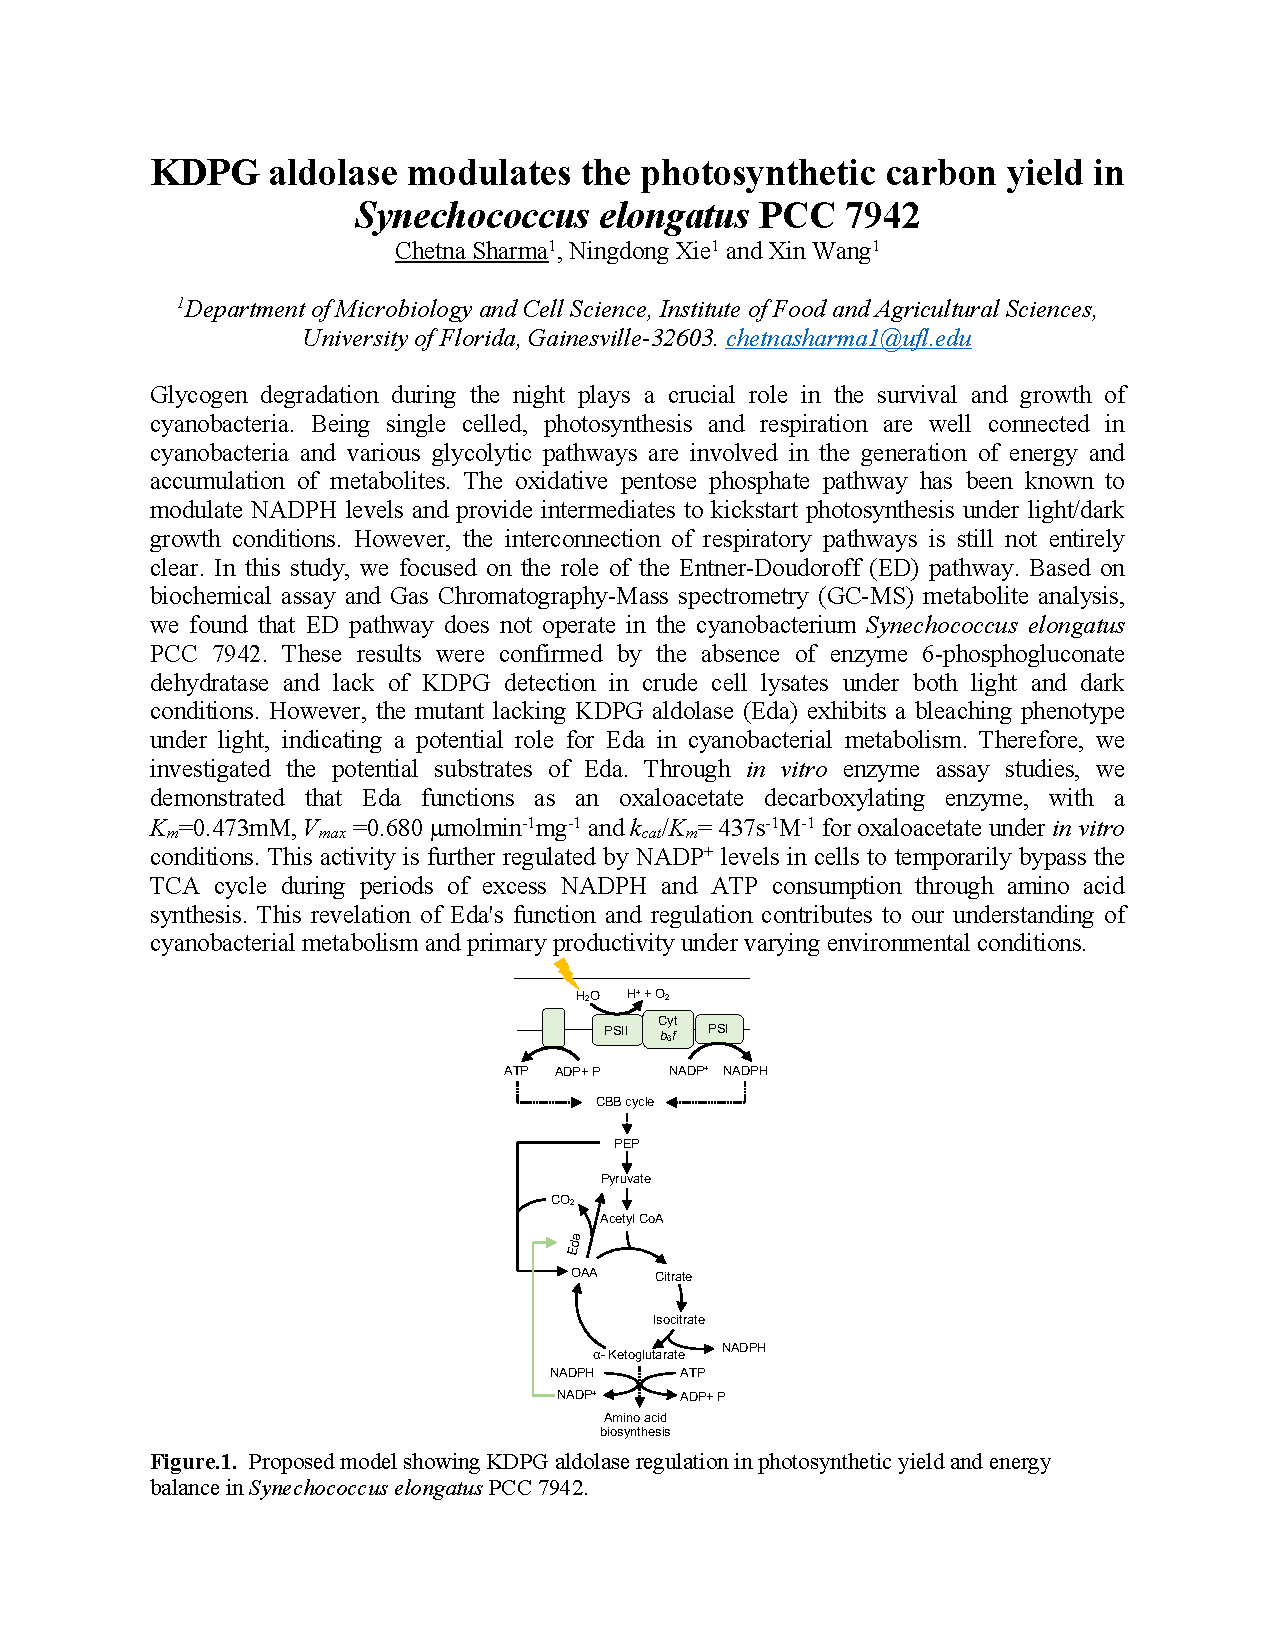
\includepdf[link=true,linkname=Sharma,pagecommand={\thispagestyle{plain}},addtolist={1,talk,heading,abs:Sharma}]{abstracts/Sharma_MWSE50.pdf}
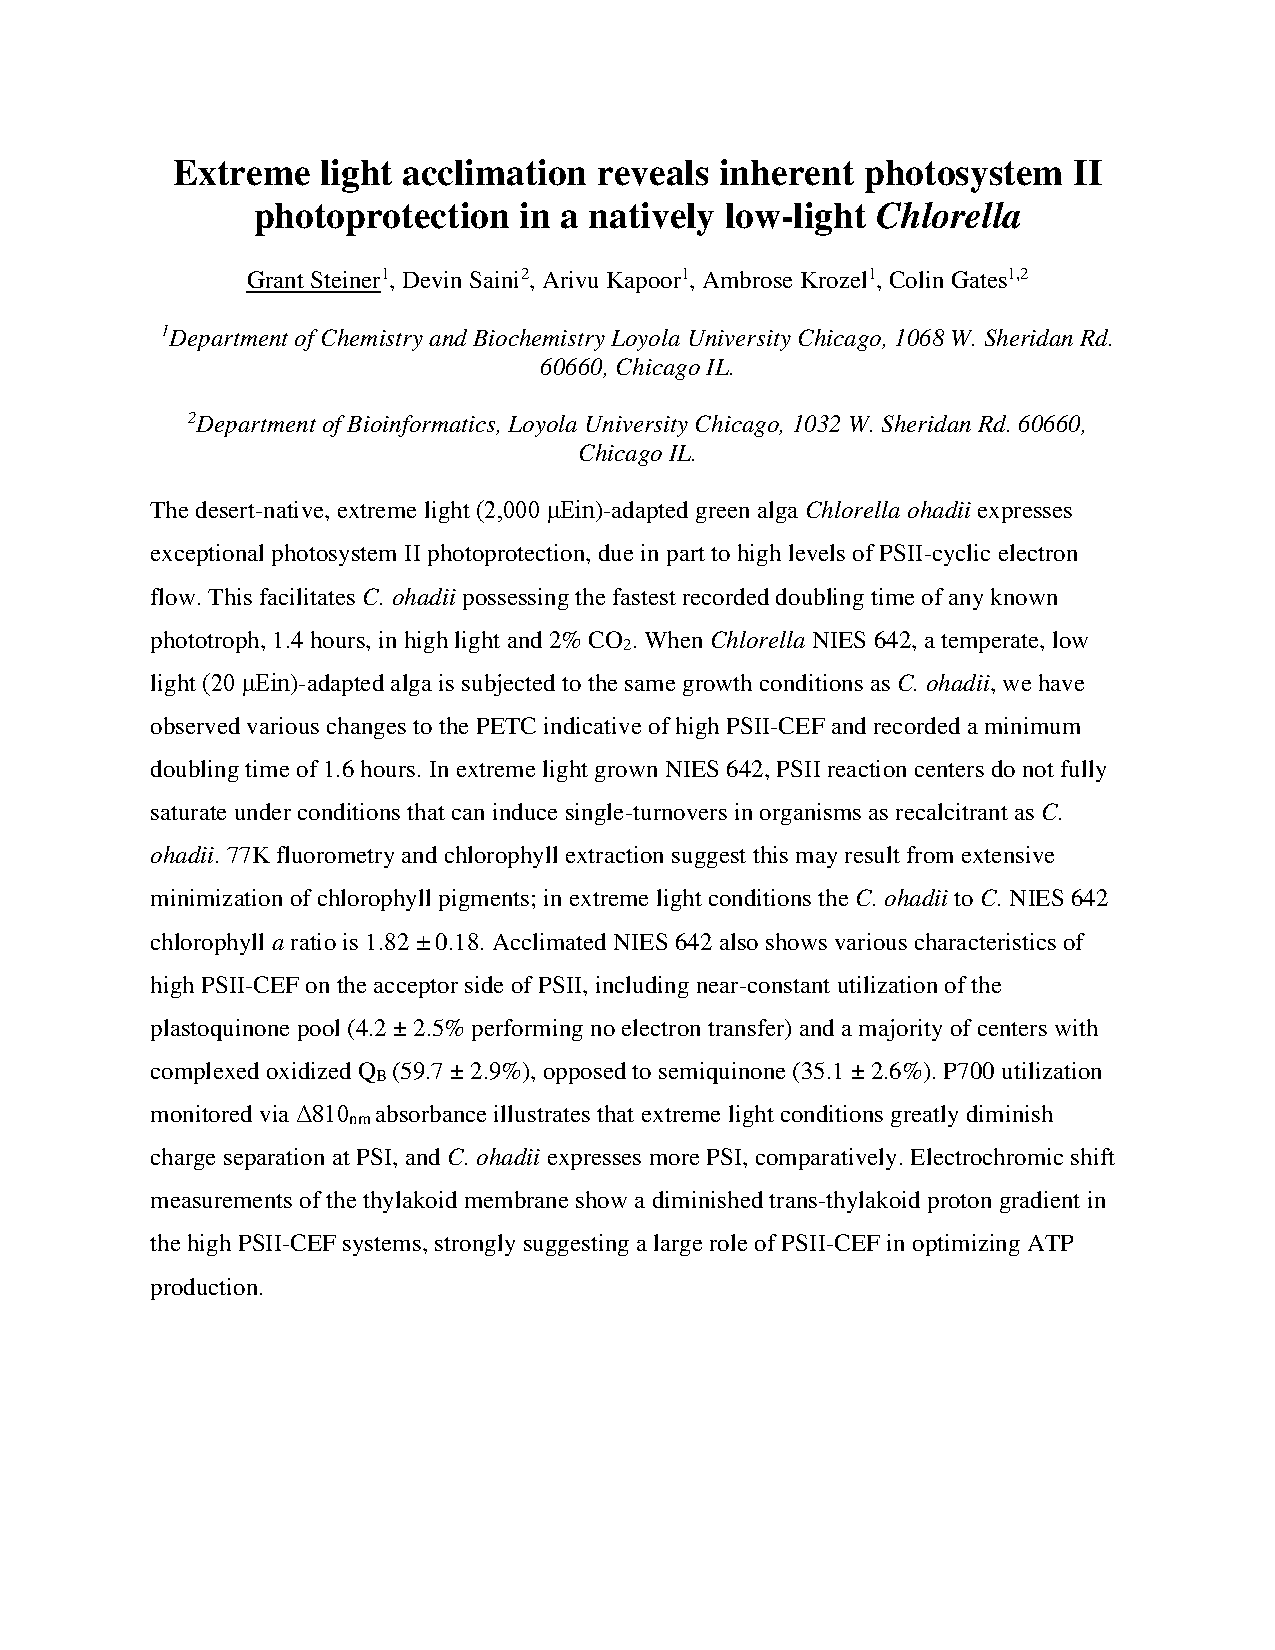
\includepdf[link=true,linkname=Steiner,pagecommand={\thispagestyle{plain}},addtolist={1,talk,heading,abs:Steiner}]{abstracts/Steiner_MWSE50.pdf}
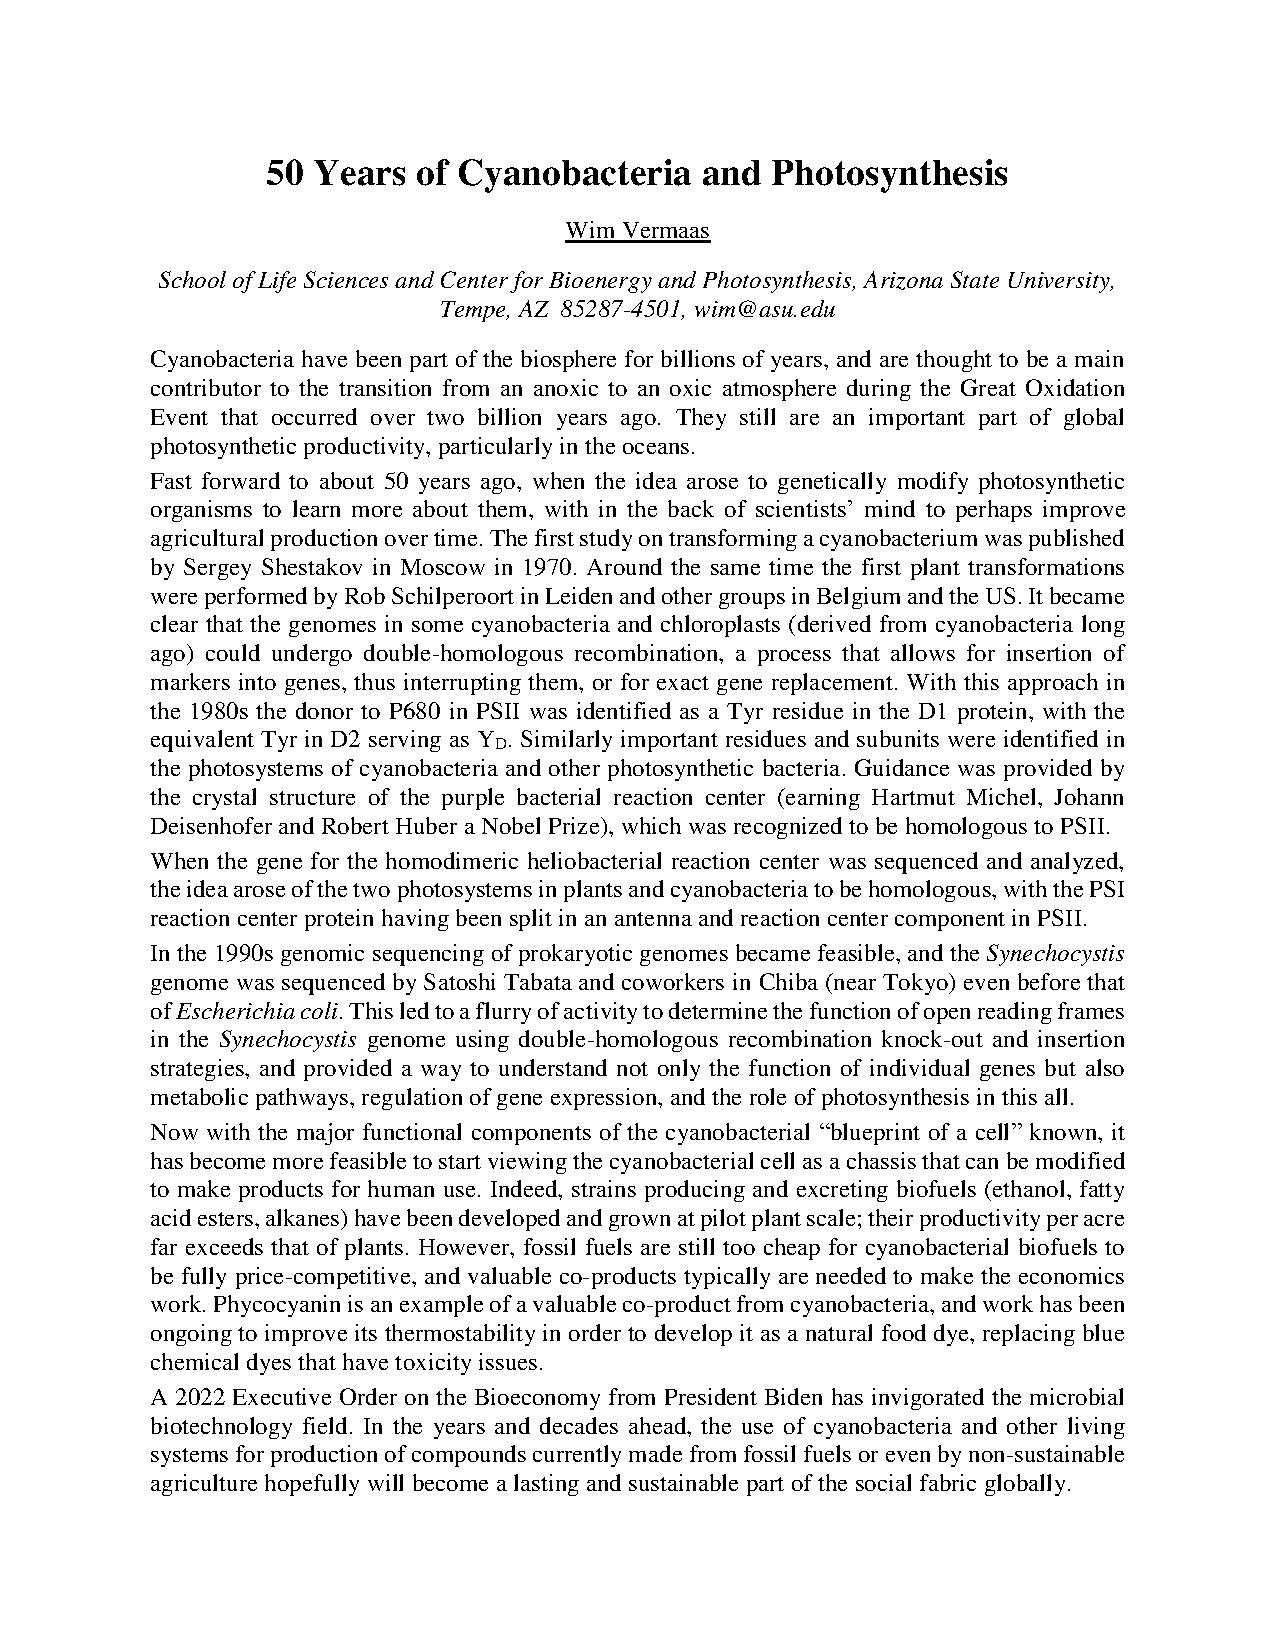
\includepdf[link=true,linkname=Vermaas,pagecommand={\thispagestyle{plain}},addtolist={1,talk,heading,abs:Vermaas}]{abstracts/Vermaas_MWSE50_Wim.pdf}
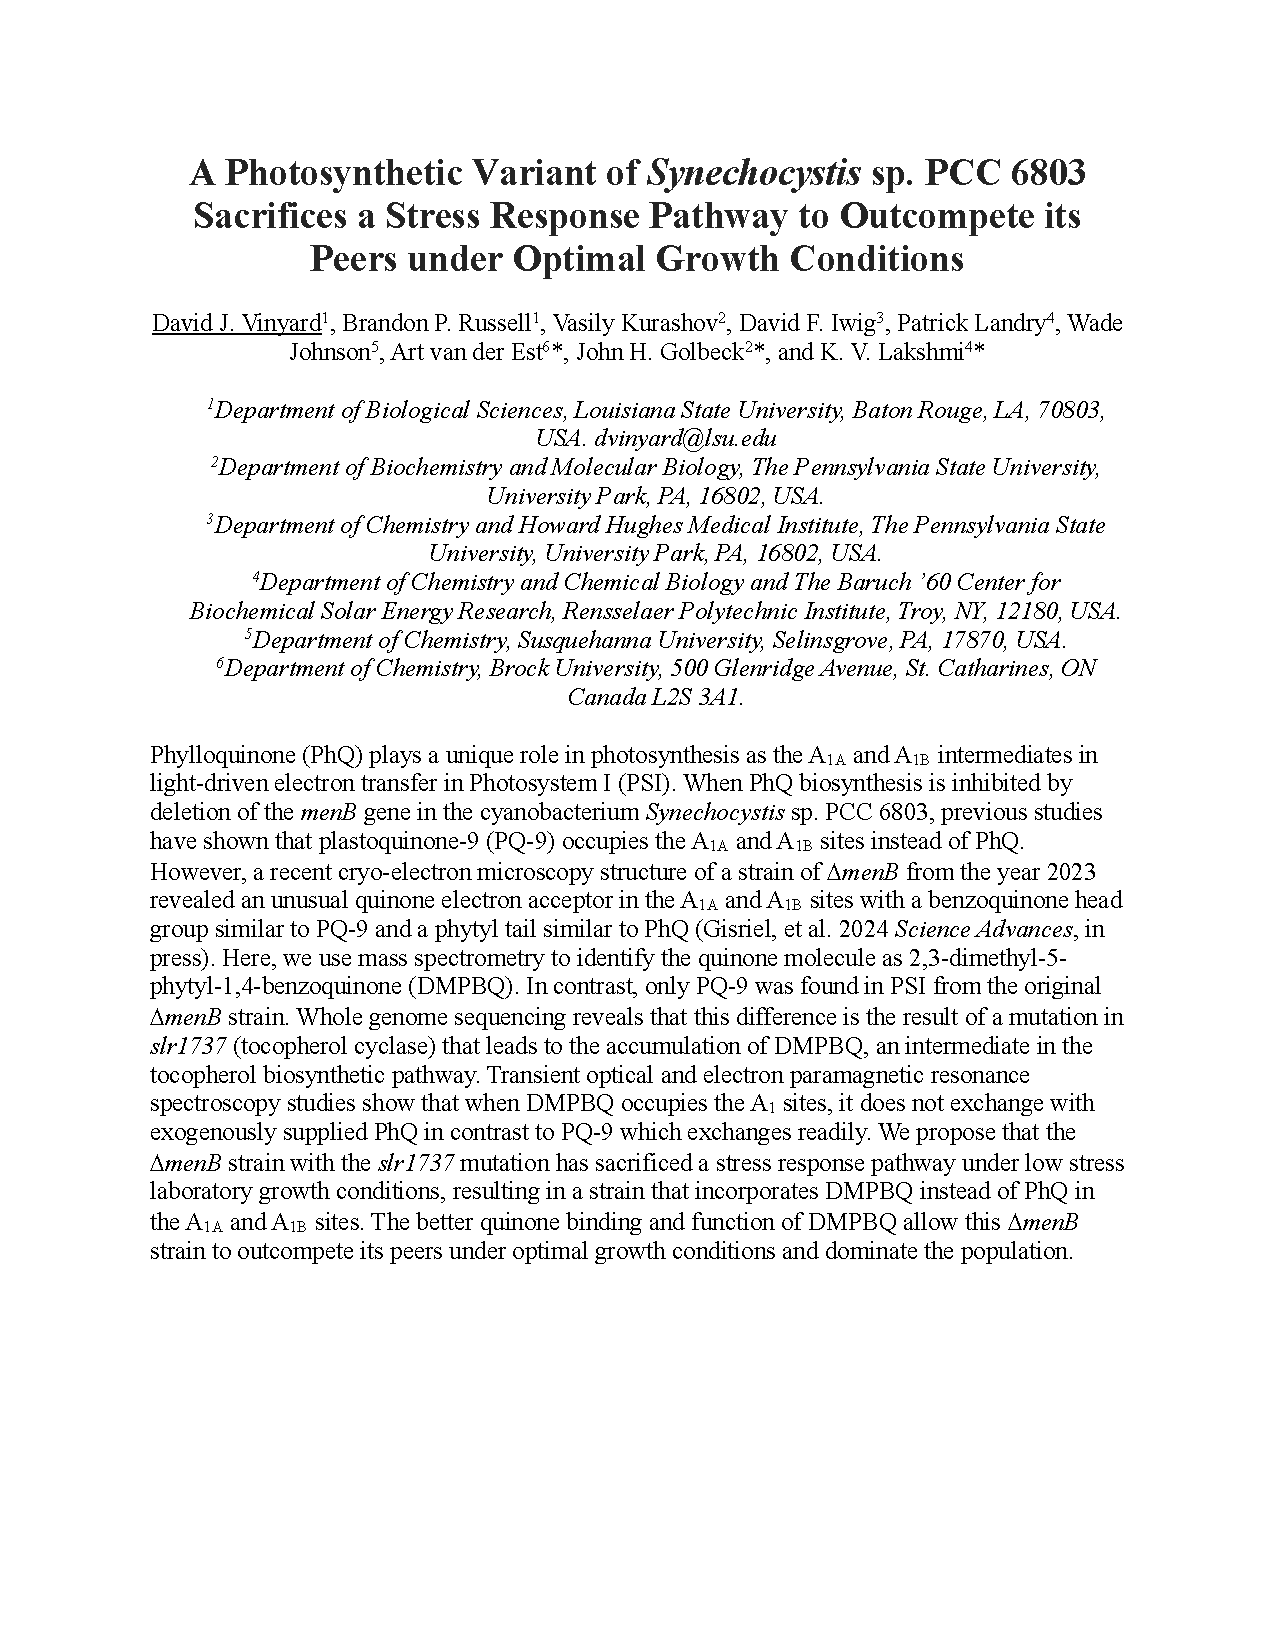
\includepdf[link=true,linkname=Vinyard,pagecommand={\thispagestyle{plain}},addtolist={1,talk,heading,abs:Vinyard}]{abstracts/Vinyard_MWSE50.pdf}


%----------------------------------------------------------------------------------------
%	 LIST OF POSTERS
%----------------------------------------------------------------------------------------

\chapter{Poster Abstracts} 
\begin{multicols}{3}
\begin{itemize}
	\item \hyperlink{Alamin.1}{Alamin} pg. \pageref{abs:Alamin}
\item \hyperlink{Arhin.1}{Arhin} pg. \pageref{abs:Arhin}
\item \hyperlink{Bandyopadhyay.1}{Bandyopadhyay} pg. \pageref{abs:Bandyopadhyay}
\item \hyperlink{Bharwad.1}{Bharwad} pg. \pageref{abs:Bharwad}
\item \hyperlink{Bhowmick.1}{Bhowmick} pg. \pageref{abs:Bhowmick}
\item \hyperlink{Biswas.1}{Biswas} pg. \pageref{abs:Biswas}
\item \hyperlink{Boren.1}{Boren} pg. \pageref{abs:Boren}
\item \hyperlink{Carpenter.1}{Carpenter} pg. \pageref{abs:Carpenter}
\item \hyperlink{Castillo.1}{Castillo} pg. \pageref{abs:Castillo}
\item \hyperlink{Chang.1}{Chang} pg. \pageref{abs:Chang}
\item \hyperlink{Dadwal.1}{Dadwal} pg. \pageref{abs:Dadwal}
\item \hyperlink{Daviebalogun.1}{Daviebalogun} pg. \pageref{abs:Daviebalogun}
\item \hyperlink{Dutta.1}{Dutta} pg. \pageref{abs:Dutta}
\item \hyperlink{Ferrari.1}{Ferrari} pg. \pageref{abs:Ferrari}
\item \hyperlink{Gundlapalli.1}{Gundlapalli} pg. \pageref{abs:Gundlapalli}
\item \hyperlink{Harman.1}{Harman} pg. \pageref{abs:Harman}
\item \hyperlink{Hiotaky.1}{Hiotaky} pg. \pageref{abs:Hiotaky}
\item \hyperlink{Holt.1}{Holt} pg. \pageref{abs:Holt}
\item \hyperlink{Jiang.1}{Jiang} pg. \pageref{abs:Jiang}
\item \hyperlink{Kamaradiwelaarachchige.1}{Kamaradiwelaarachchige} pg. \pageref{abs:Kamaradiwelaarachchige}
\item \hyperlink{Kapoor.1}{Kapoor} pg. \pageref{abs:Kapoor}
\item \hyperlink{Kulkarni.1}{Kulkarni} pg. \pageref{abs:Kulkarni}
\item \hyperlink{Lima.1}{Lima} pg. \pageref{abs:Lima}
\item \hyperlink{Martin.1}{Martin} pg. \pageref{abs:Martin}
\item \hyperlink{Mcginness.1}{Mcginness} pg. \pageref{abs:Mcginness}
\item \hyperlink{Mckenzie.1}{Mckenzie} pg. \pageref{abs:Mckenzie}
\item \hyperlink{Nicolaou.1}{Nicolaou} pg. \pageref{abs:Nicolaou}
\item \hyperlink{Niklas.1}{Niklas} pg. \pageref{abs:Niklas}
\item \hyperlink{Olagunju.1}{Olagunju} pg. \pageref{abs:Olagunju}
\item \hyperlink{Seifert.1}{Seifert} pg. \pageref{abs:Seifert}
\item \hyperlink{Sharpe.1}{Sharpe} pg. \pageref{abs:Sharpe}
\item \hyperlink{Short.1}{Short} pg. \pageref{abs:Short}
\item \hyperlink{Smolen.1}{Smolen} pg. \pageref{abs:Smolen}
\item \hyperlink{Snyder.1}{Snyder} pg. \pageref{abs:Snyder}
\item \hyperlink{Strong.1}{Strong} pg. \pageref{abs:Strong}
\item \hyperlink{Trembath.1}{Trembath} pg. \pageref{abs:Trembath}
\item \hyperlink{Tuncer.1}{Tuncer} pg. \pageref{abs:Tuncer}
\item \hyperlink{Weesinghe.1}{Weesinghe} pg. \pageref{abs:Weesinghe}
\item \hyperlink{Wheeless.1}{Wheeless} pg. \pageref{abs:Wheeless}
\item \hyperlink{Williams.1}{Williams} pg. \pageref{abs:Williams}
\item \hyperlink{Yadav.1}{Yadav} pg. \pageref{abs:Yadav}

\end{itemize}
\end{multicols}
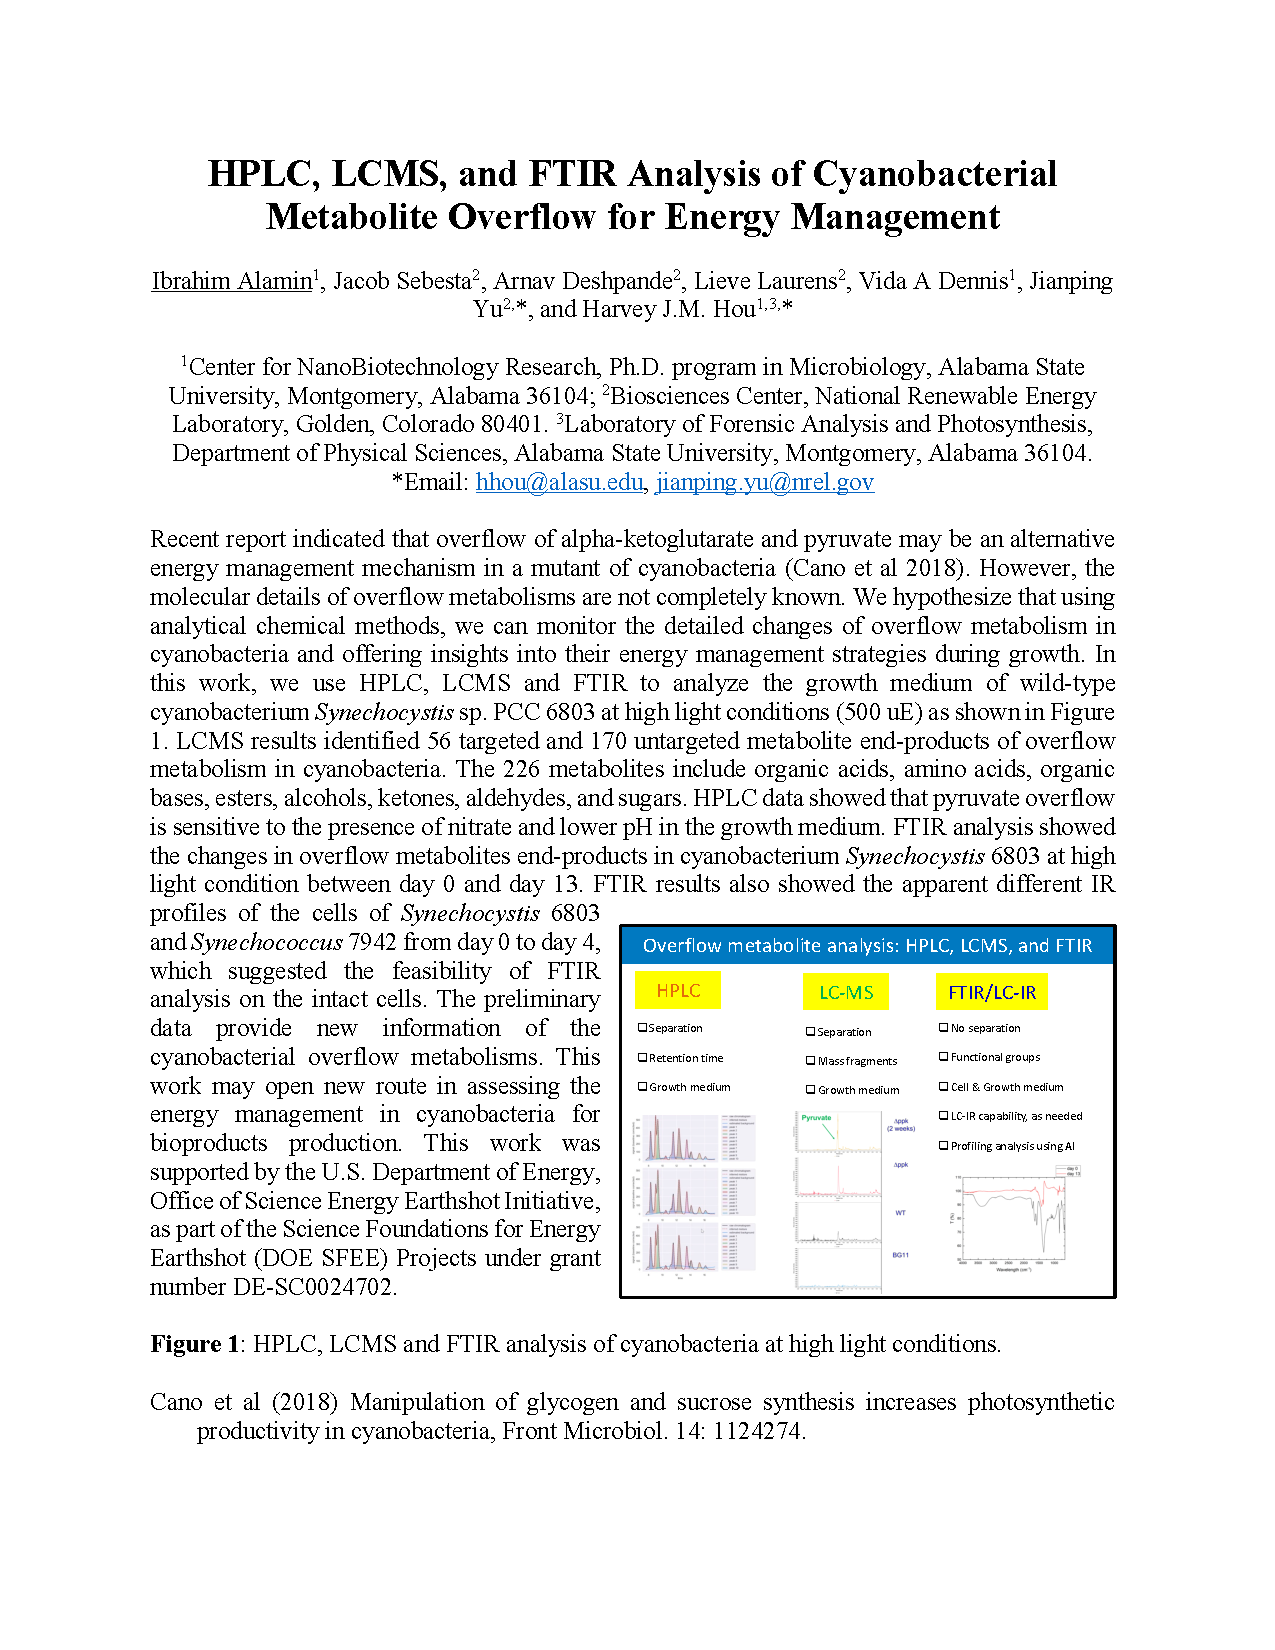
\includepdf[link=true,linkname=Alamin,pagecommand={\thispagestyle{plain}},addtolist={1,nottalk,heading,abs:Alamin}]{abstracts/alamin_MWSE50.pdf}
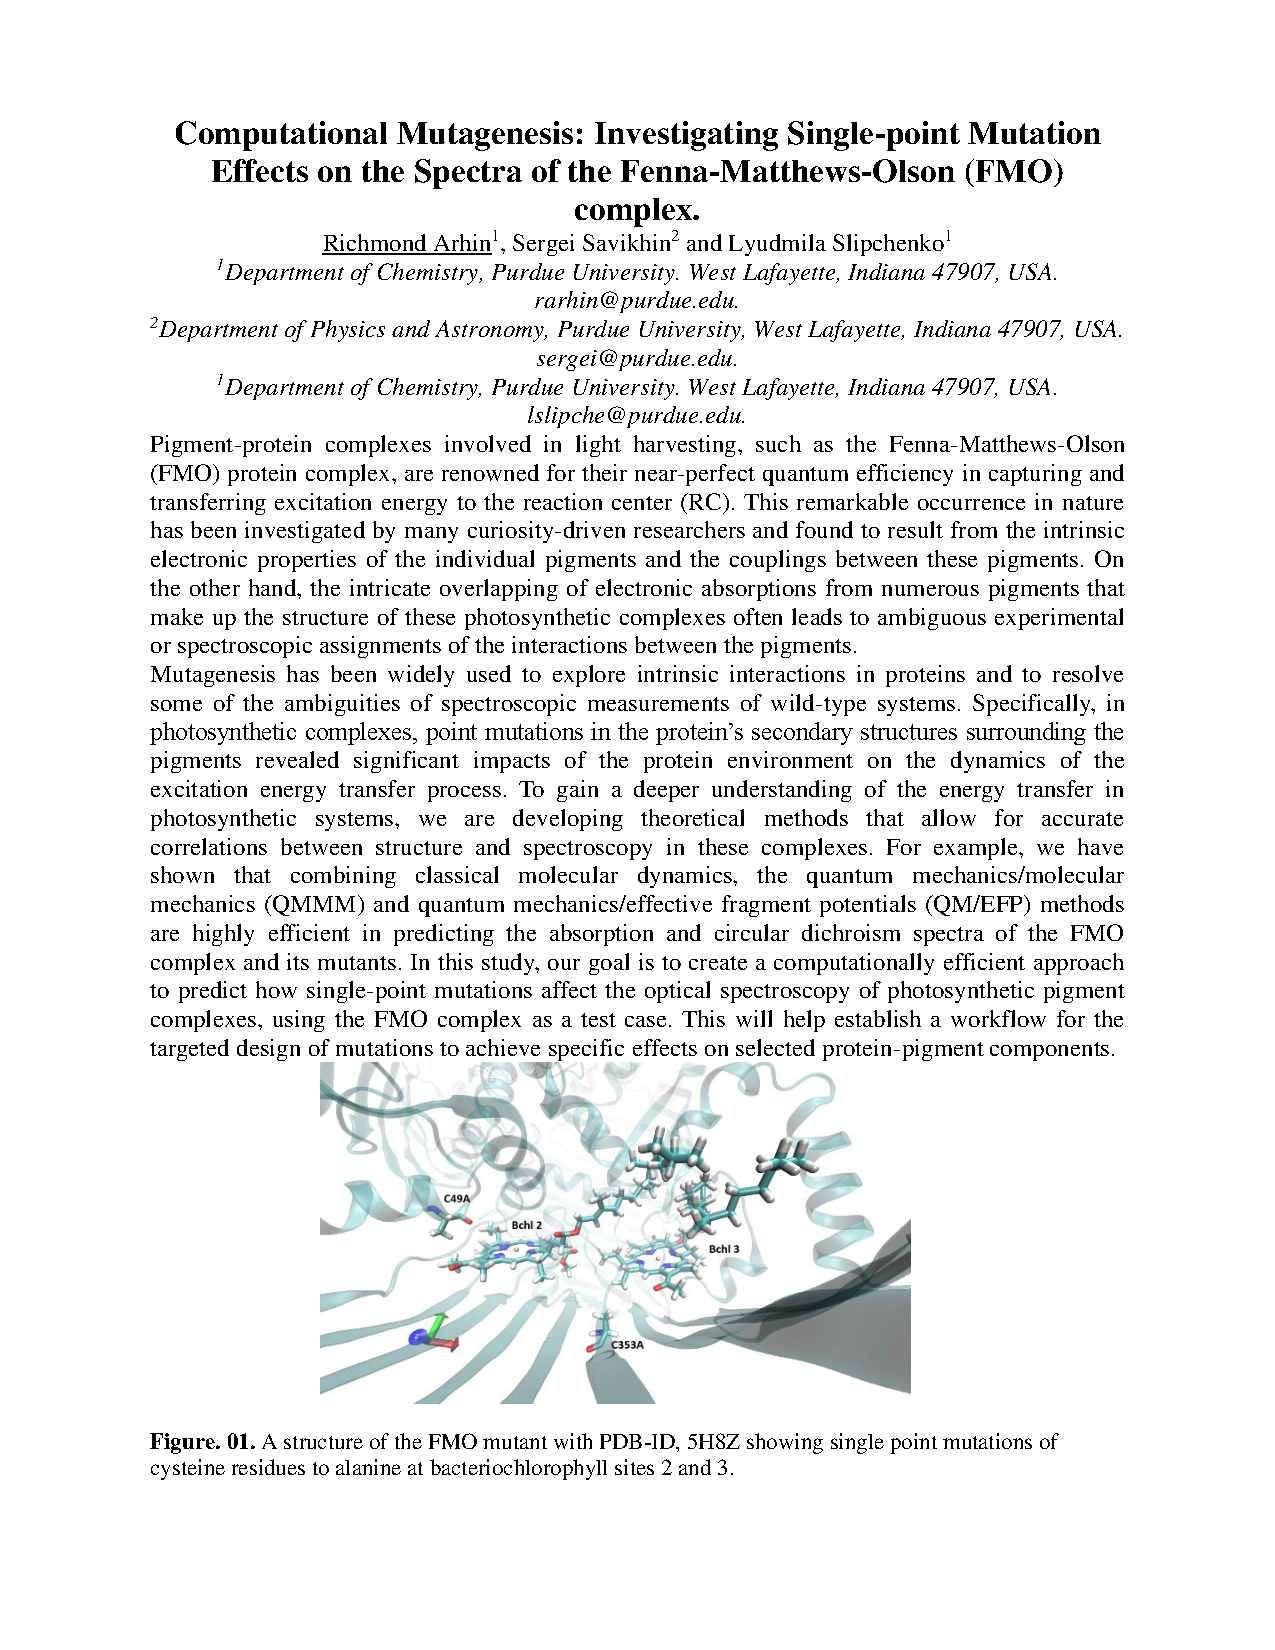
\includepdf[link=true,linkname=Arhin,pagecommand={\thispagestyle{plain}},addtolist={1,nottalk,heading,abs:Arhin}]{abstracts/Arhin_MWSE50.pdf}
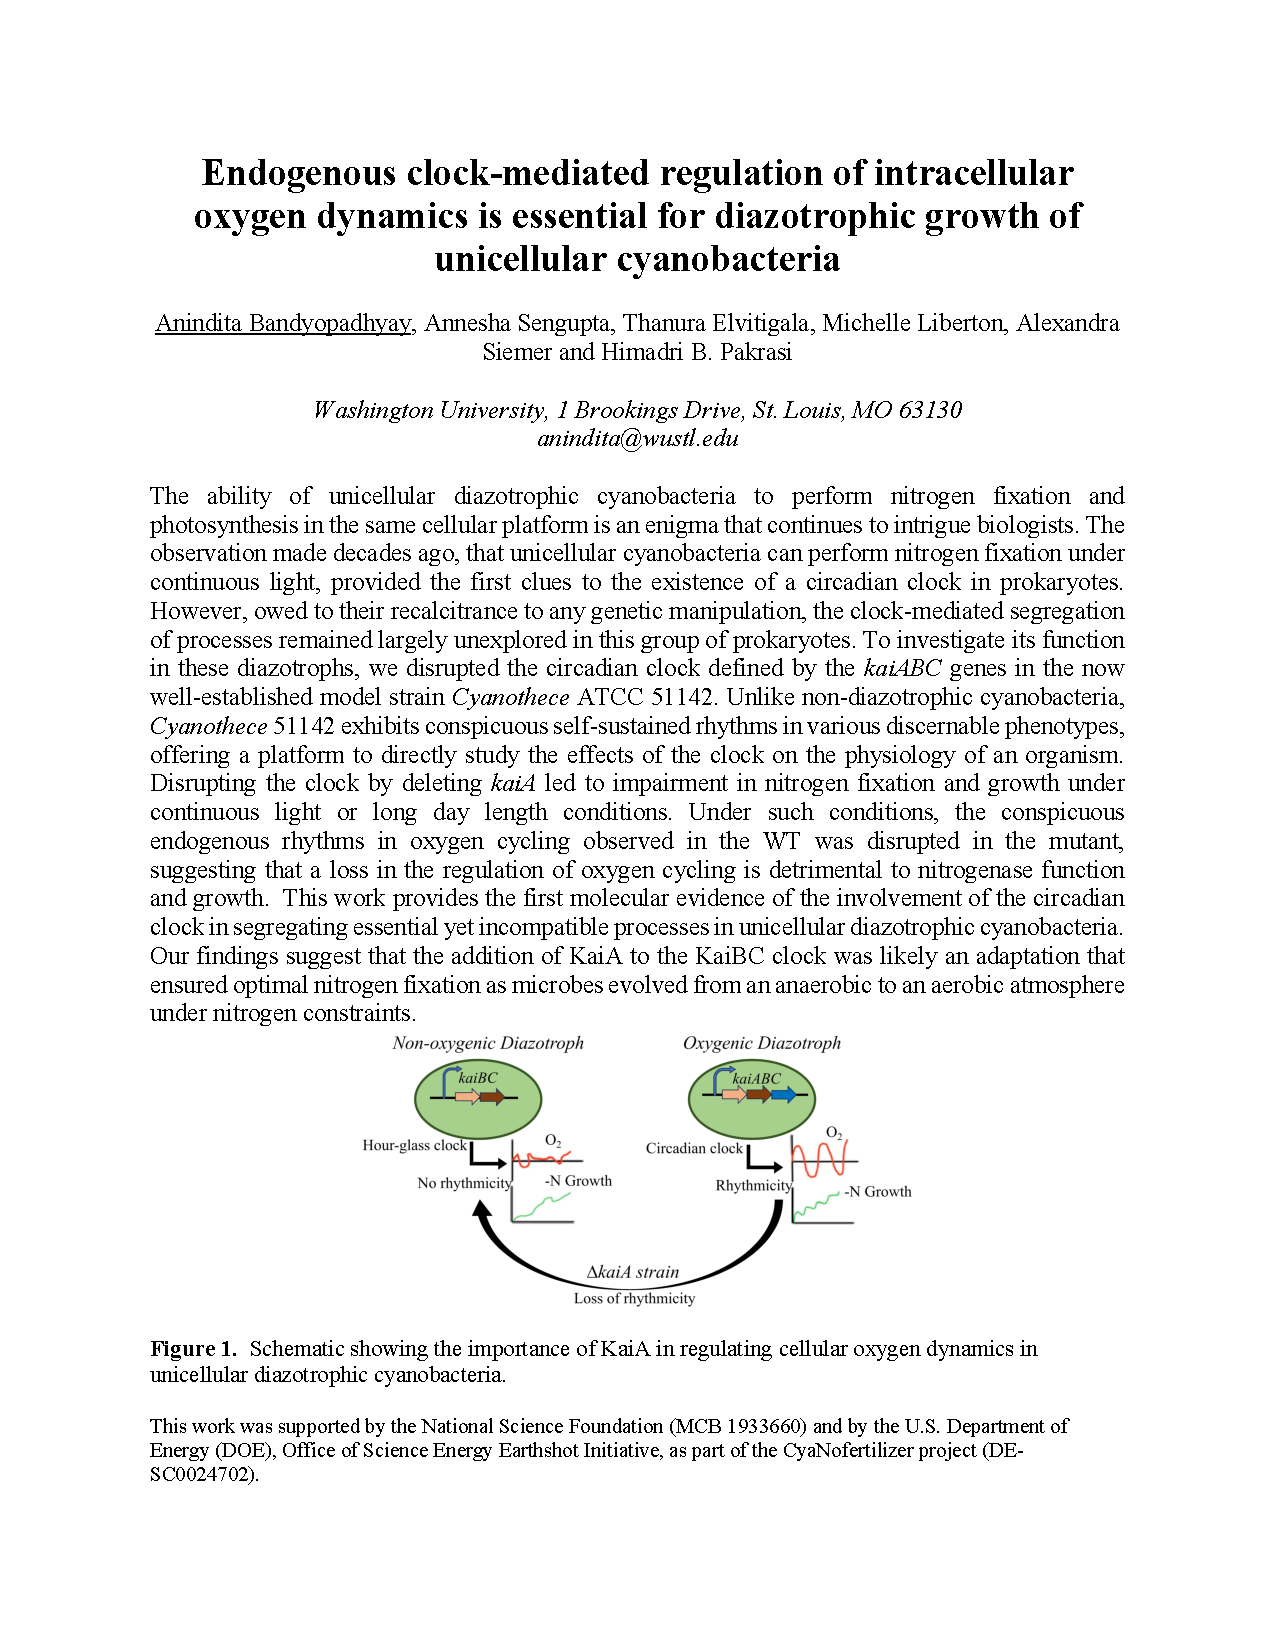
\includepdf[link=true,linkname=Bandyopadhyay,pagecommand={\thispagestyle{plain}},addtolist={1,nottalk,heading,abs:Bandyopadhyay}]{abstracts/Bandyopadhyay_MWSE50.pdf}
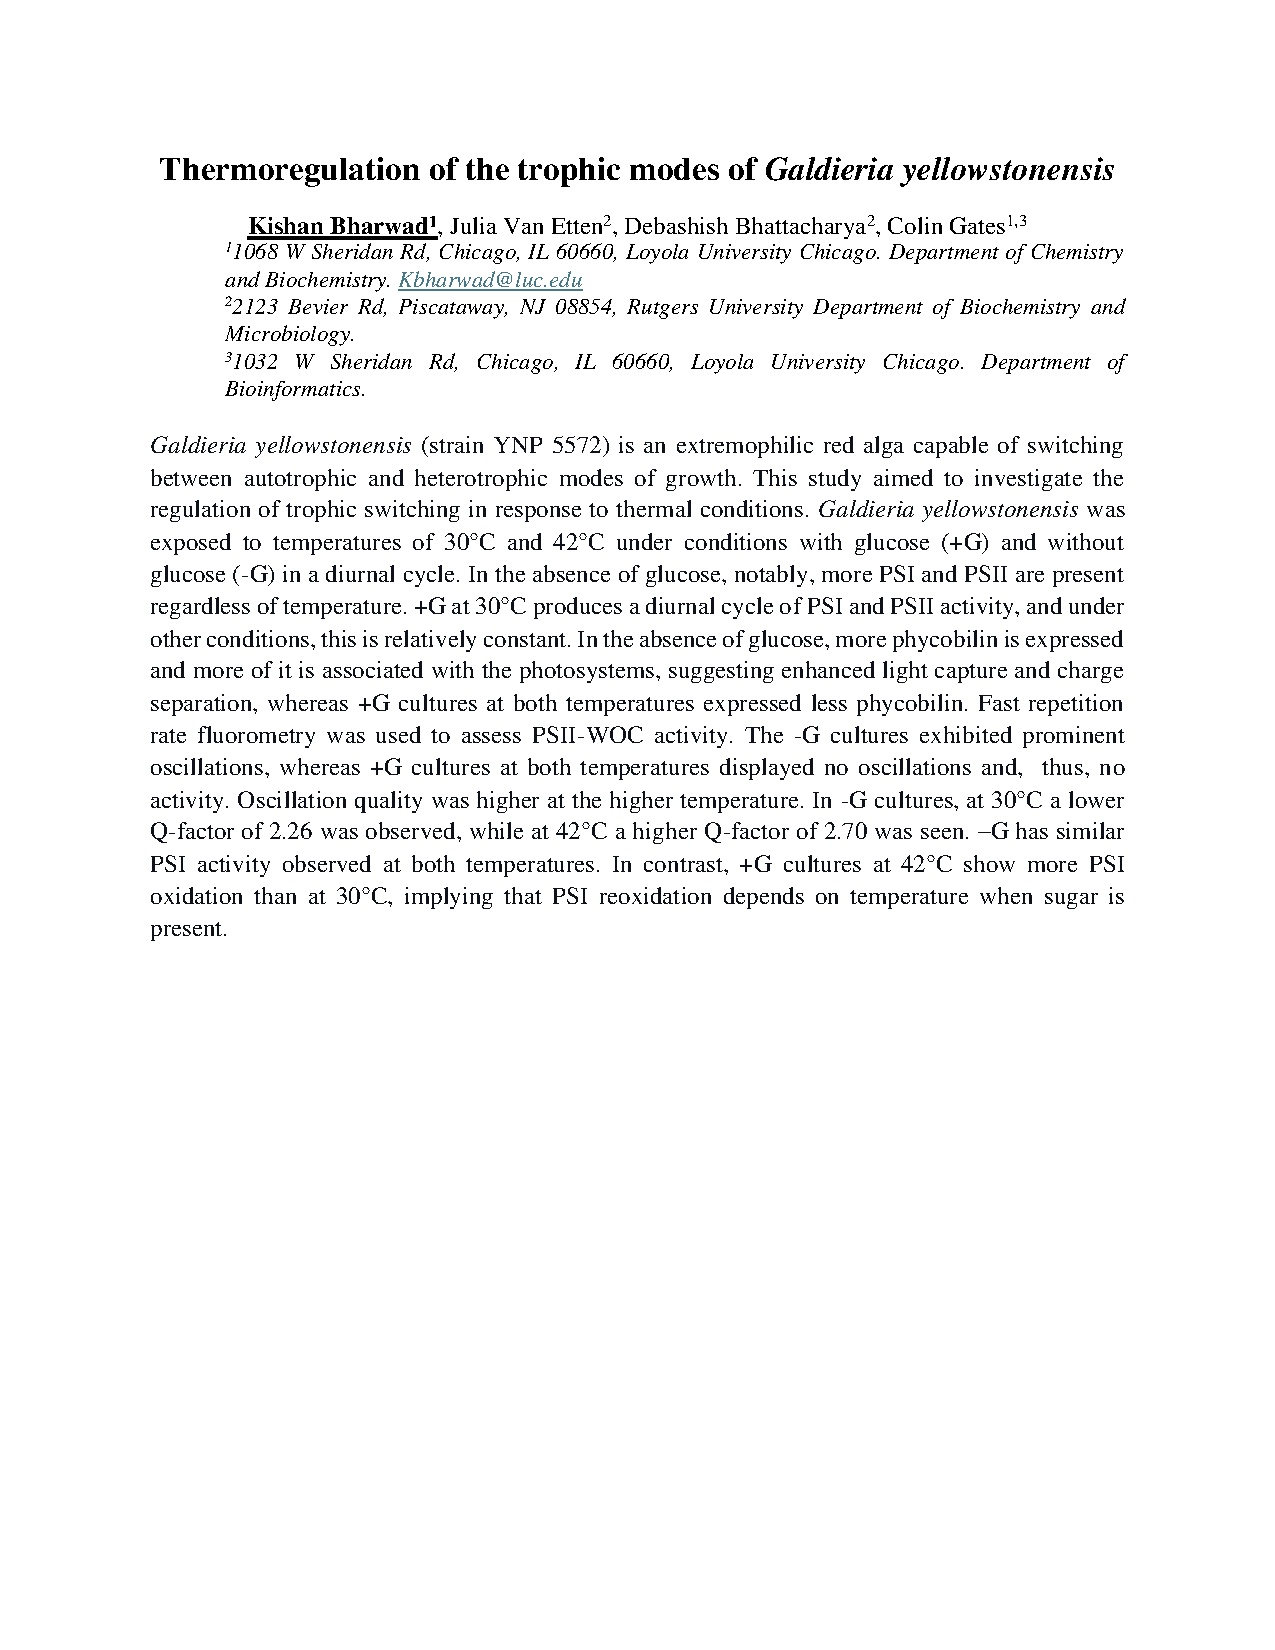
\includepdf[link=true,linkname=Bharwad,pagecommand={\thispagestyle{plain}},addtolist={1,nottalk,heading,abs:Bharwad}]{abstracts/Bharwad_MWSE50.pdf}
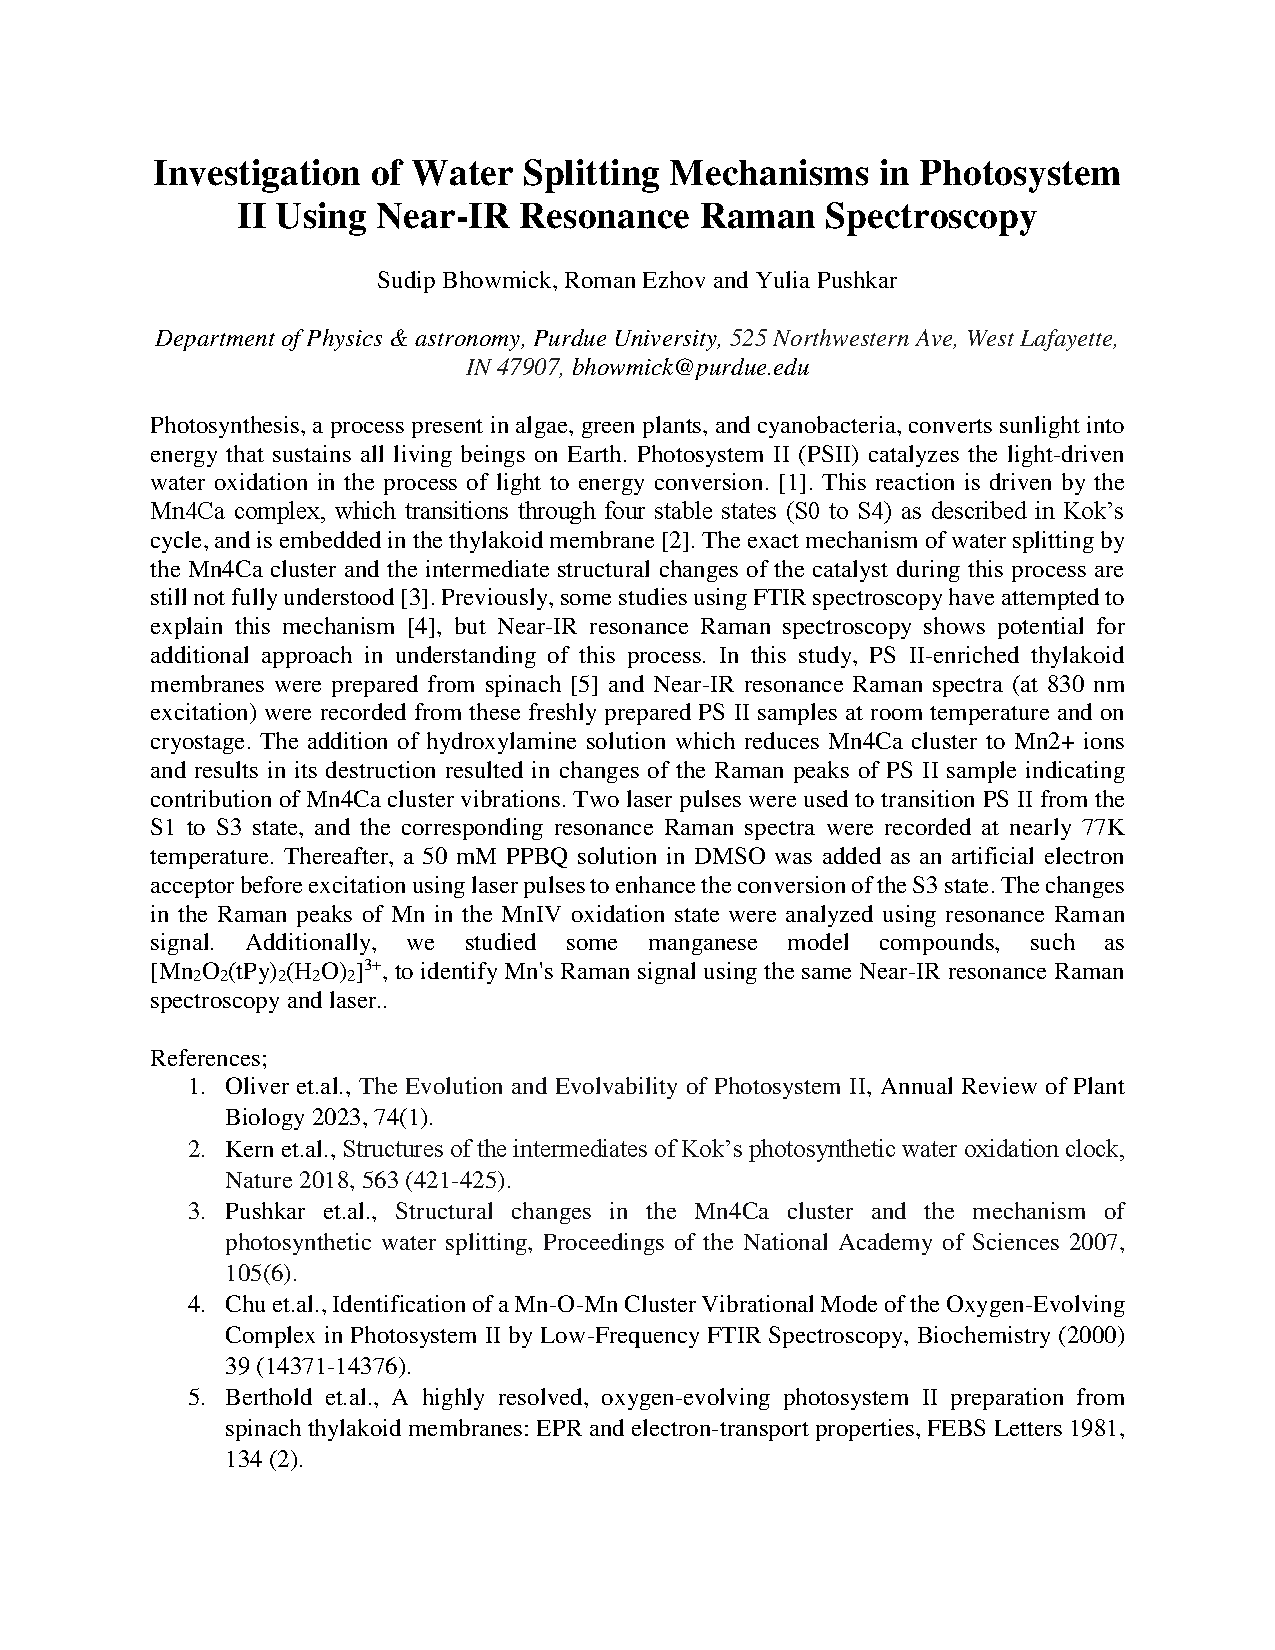
\includepdf[link=true,linkname=Bhowmick,pagecommand={\thispagestyle{plain}},addtolist={1,nottalk,heading,abs:Bhowmick}]{abstracts/Bhowmick_MWSE50.pdf}
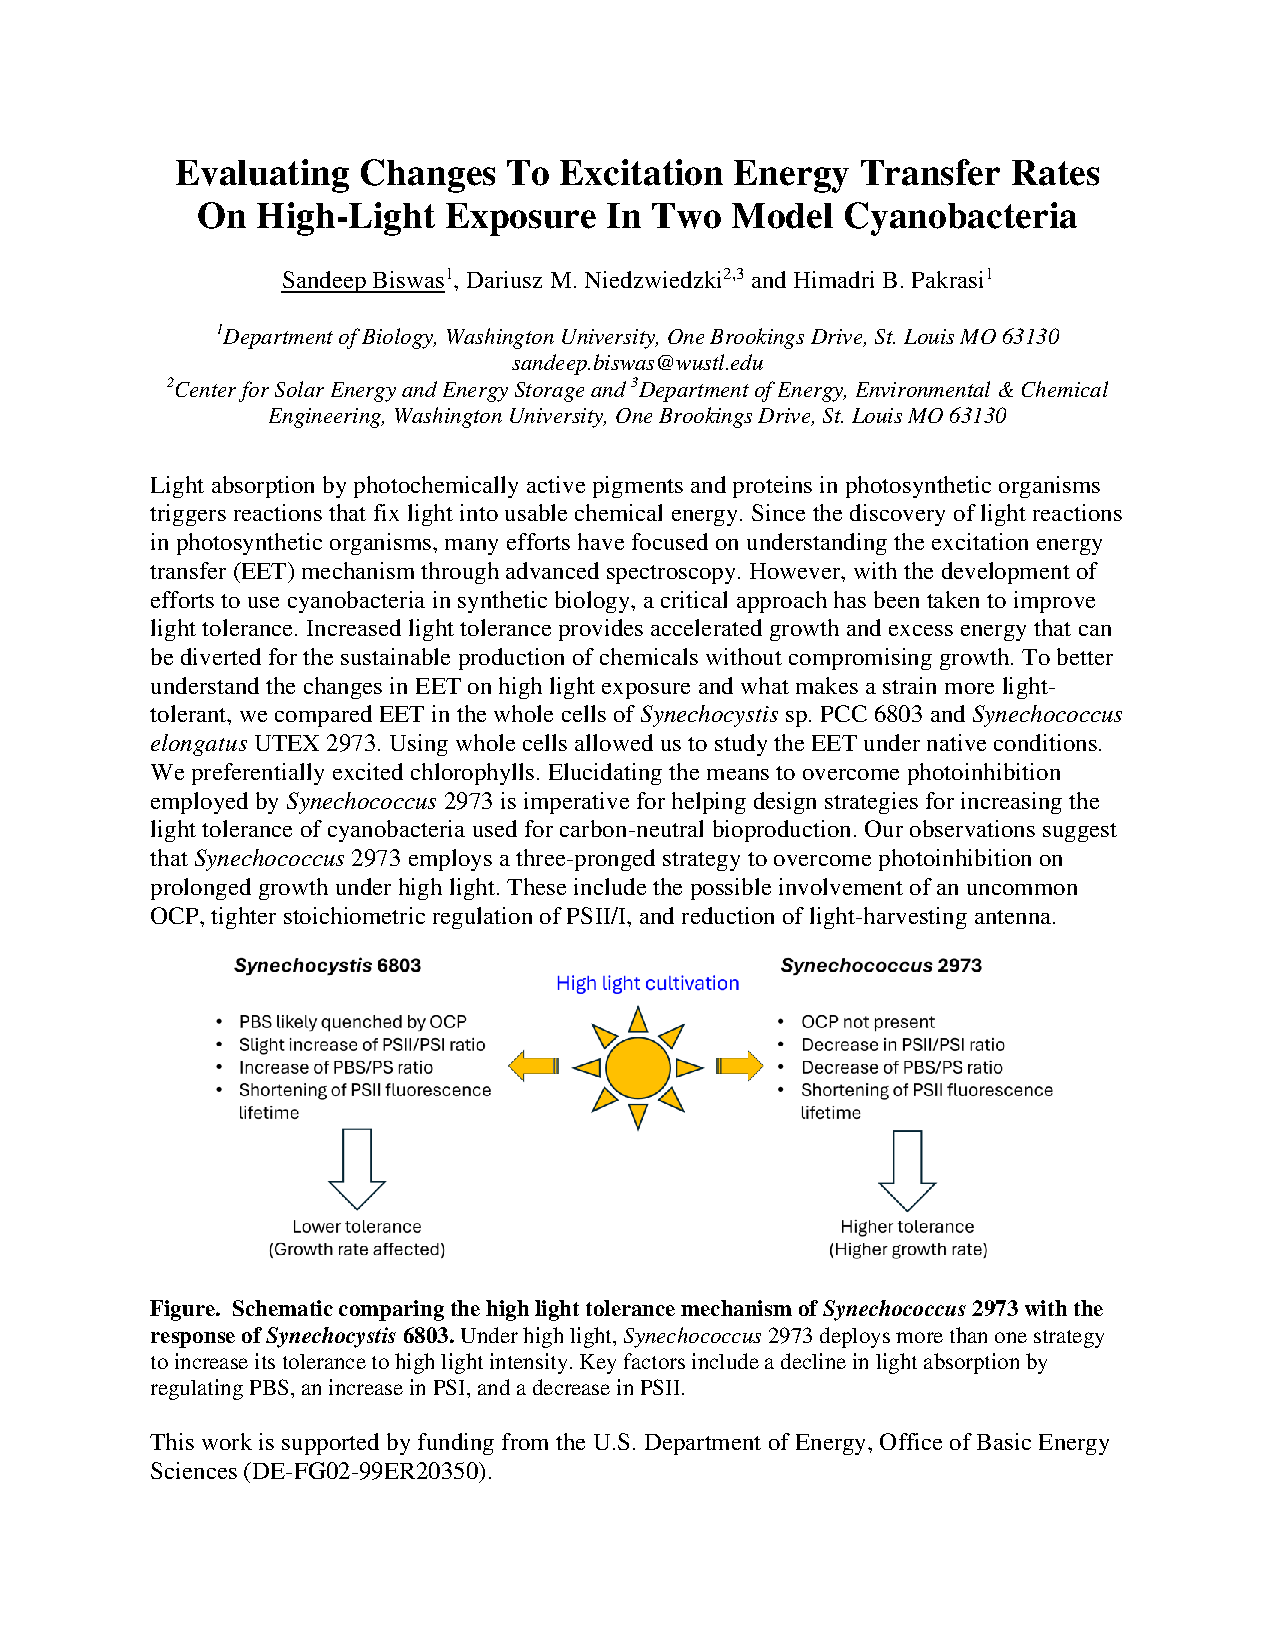
\includepdf[link=true,linkname=Biswas,pagecommand={\thispagestyle{plain}},addtolist={1,nottalk,heading,abs:Biswas}]{abstracts/Biswas_MWSE50.pdf}
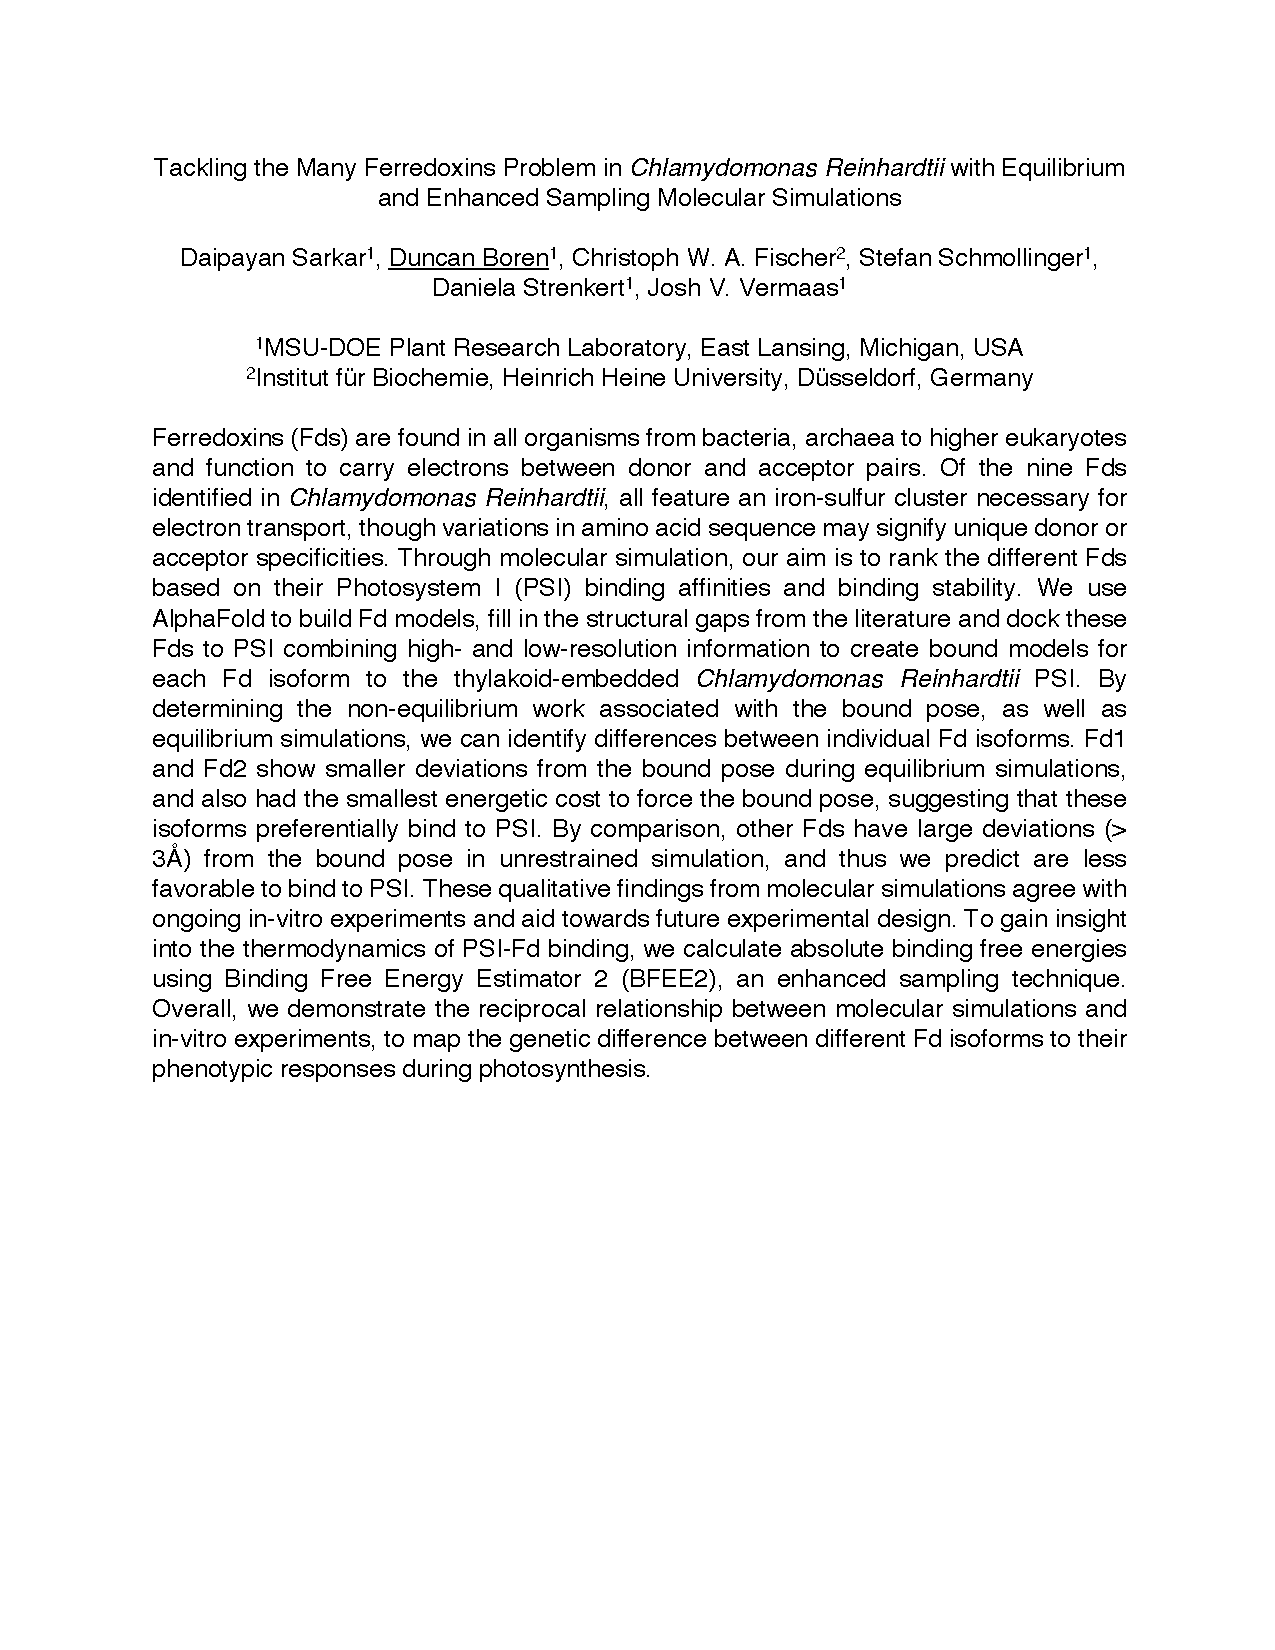
\includepdf[link=true,linkname=Boren,pagecommand={\thispagestyle{plain}},addtolist={1,nottalk,heading,abs:Boren}]{abstracts/Boren_MWSE50.pdf}
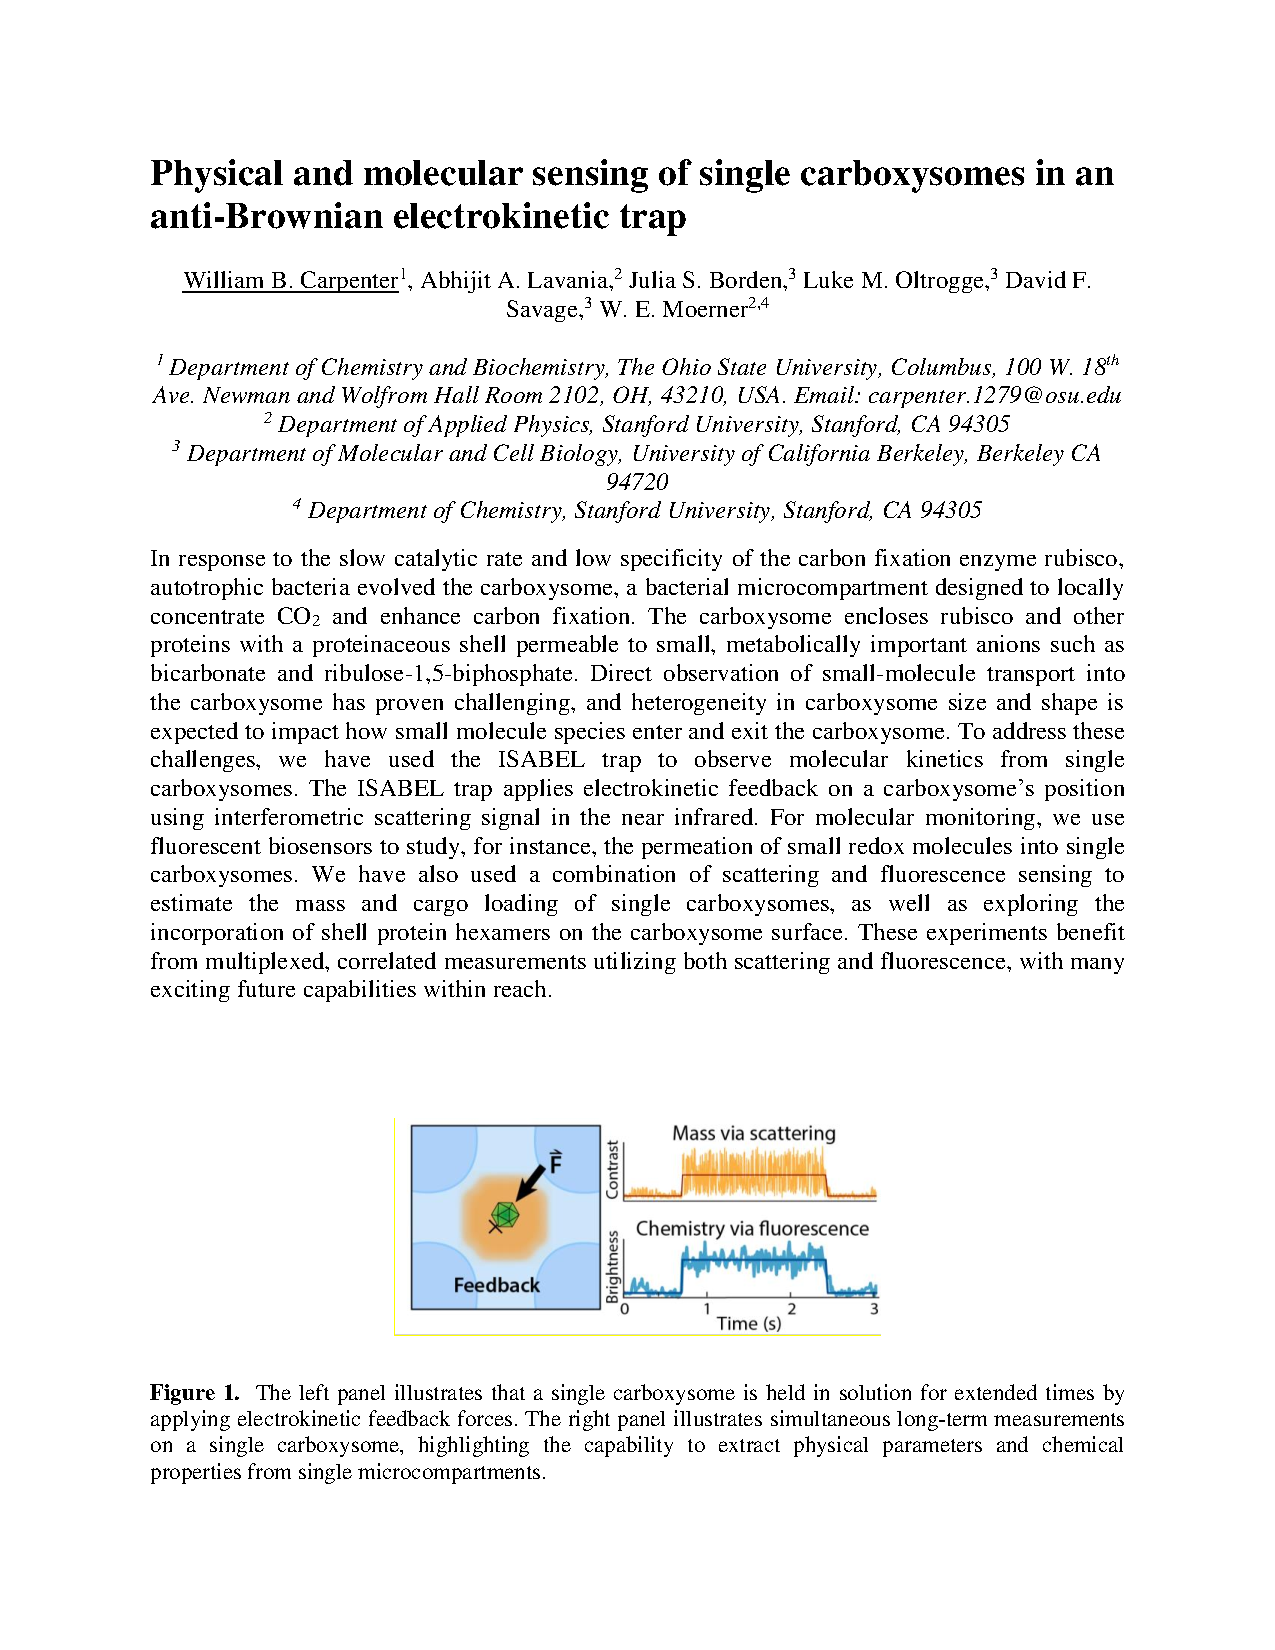
\includepdf[link=true,linkname=Carpenter,pagecommand={\thispagestyle{plain}},addtolist={1,nottalk,heading,abs:Carpenter}]{abstracts/Carpenter_MWSE50.pdf}
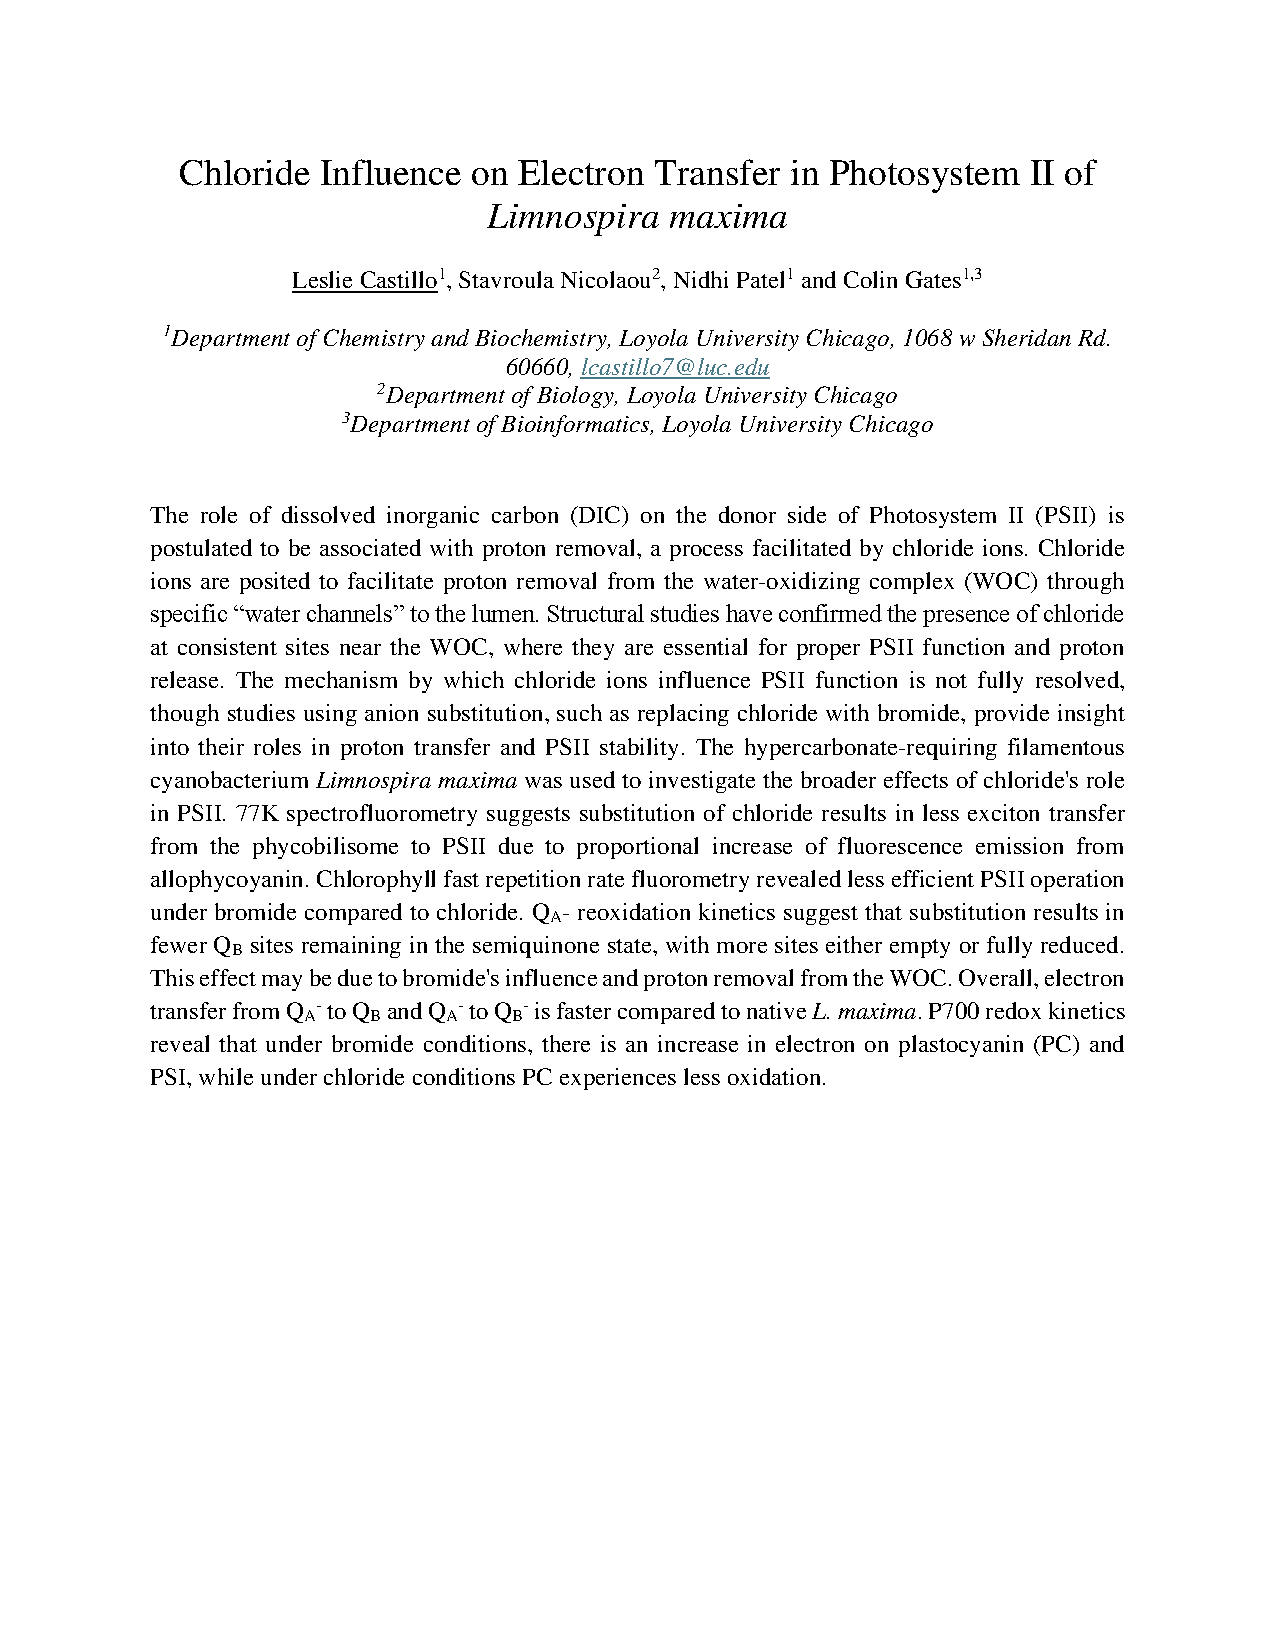
\includepdf[link=true,linkname=Castillo,pagecommand={\thispagestyle{plain}},addtolist={1,nottalk,heading,abs:Castillo}]{abstracts/Castillo_MWSE50.pdf}
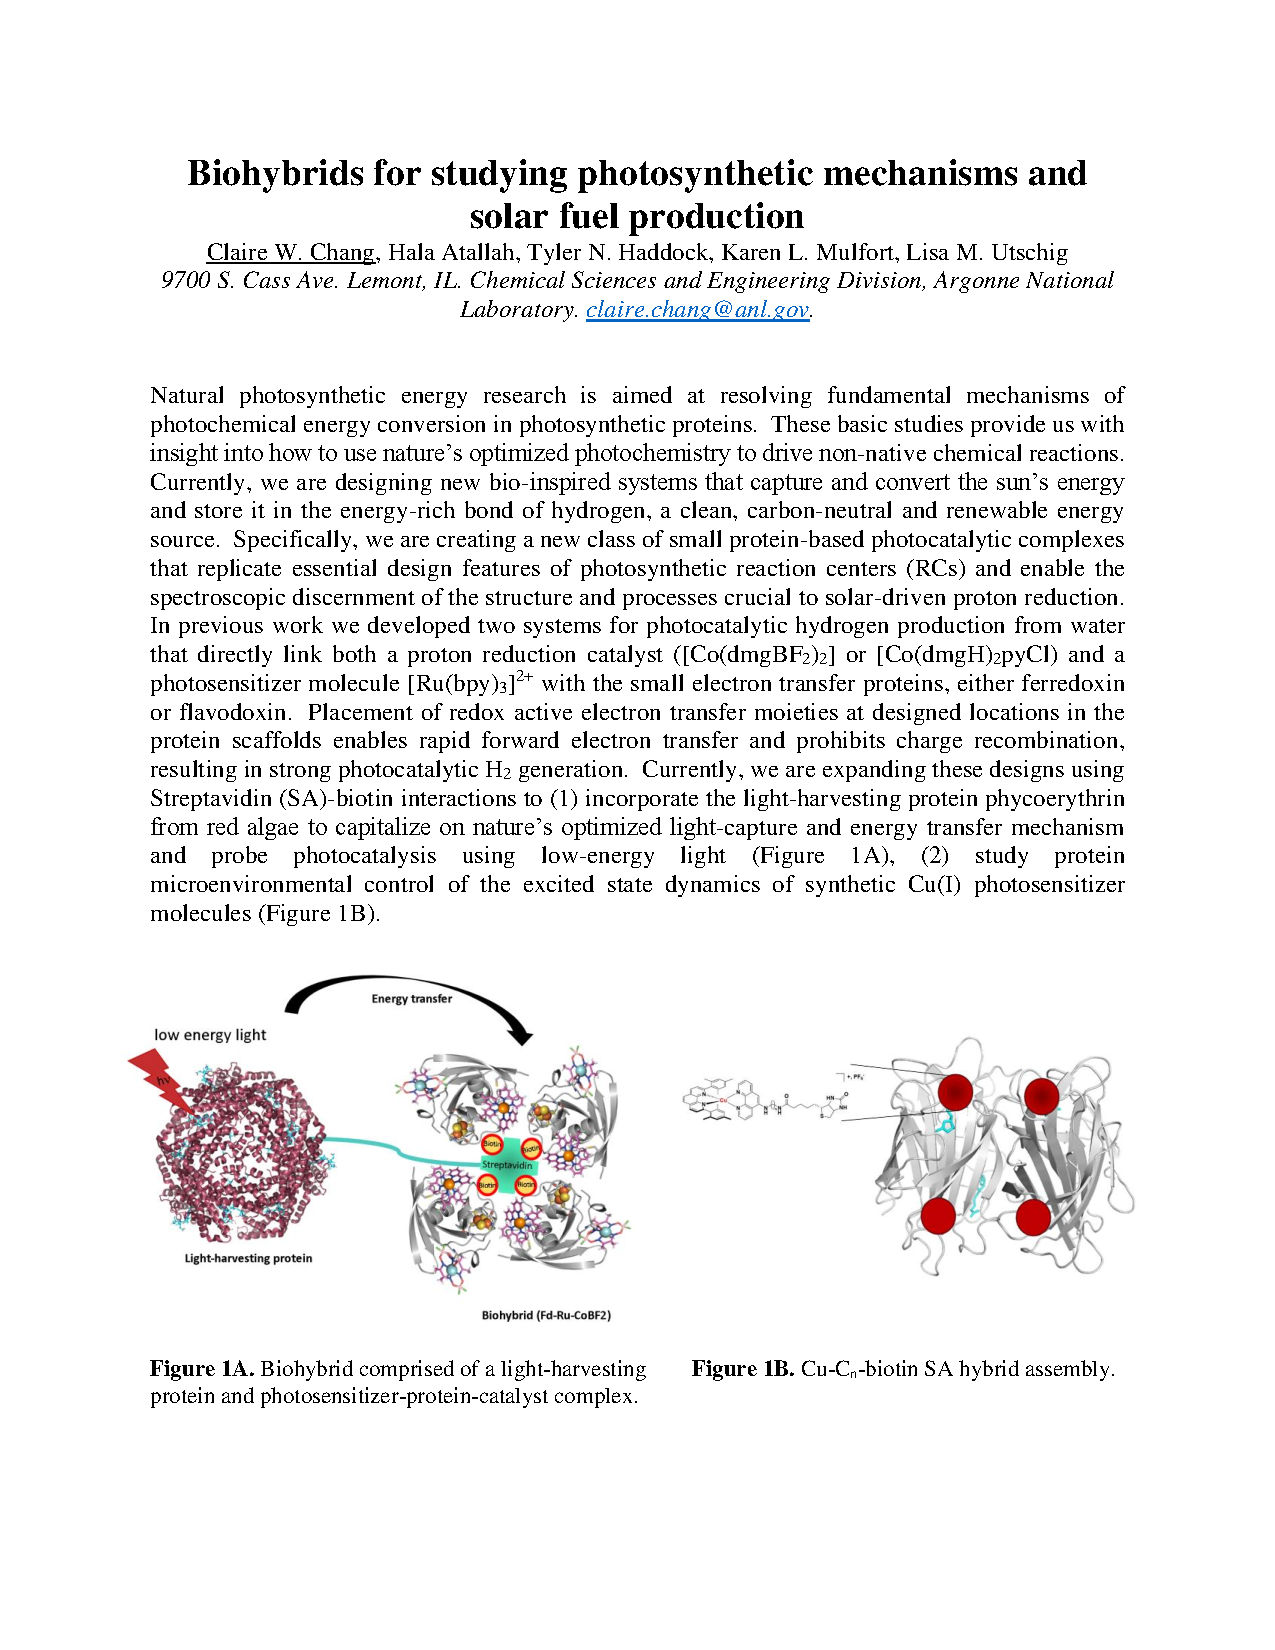
\includepdf[link=true,linkname=Chang,pagecommand={\thispagestyle{plain}},addtolist={1,nottalk,heading,abs:Chang}]{abstracts/Chang_MWSE50.pdf}
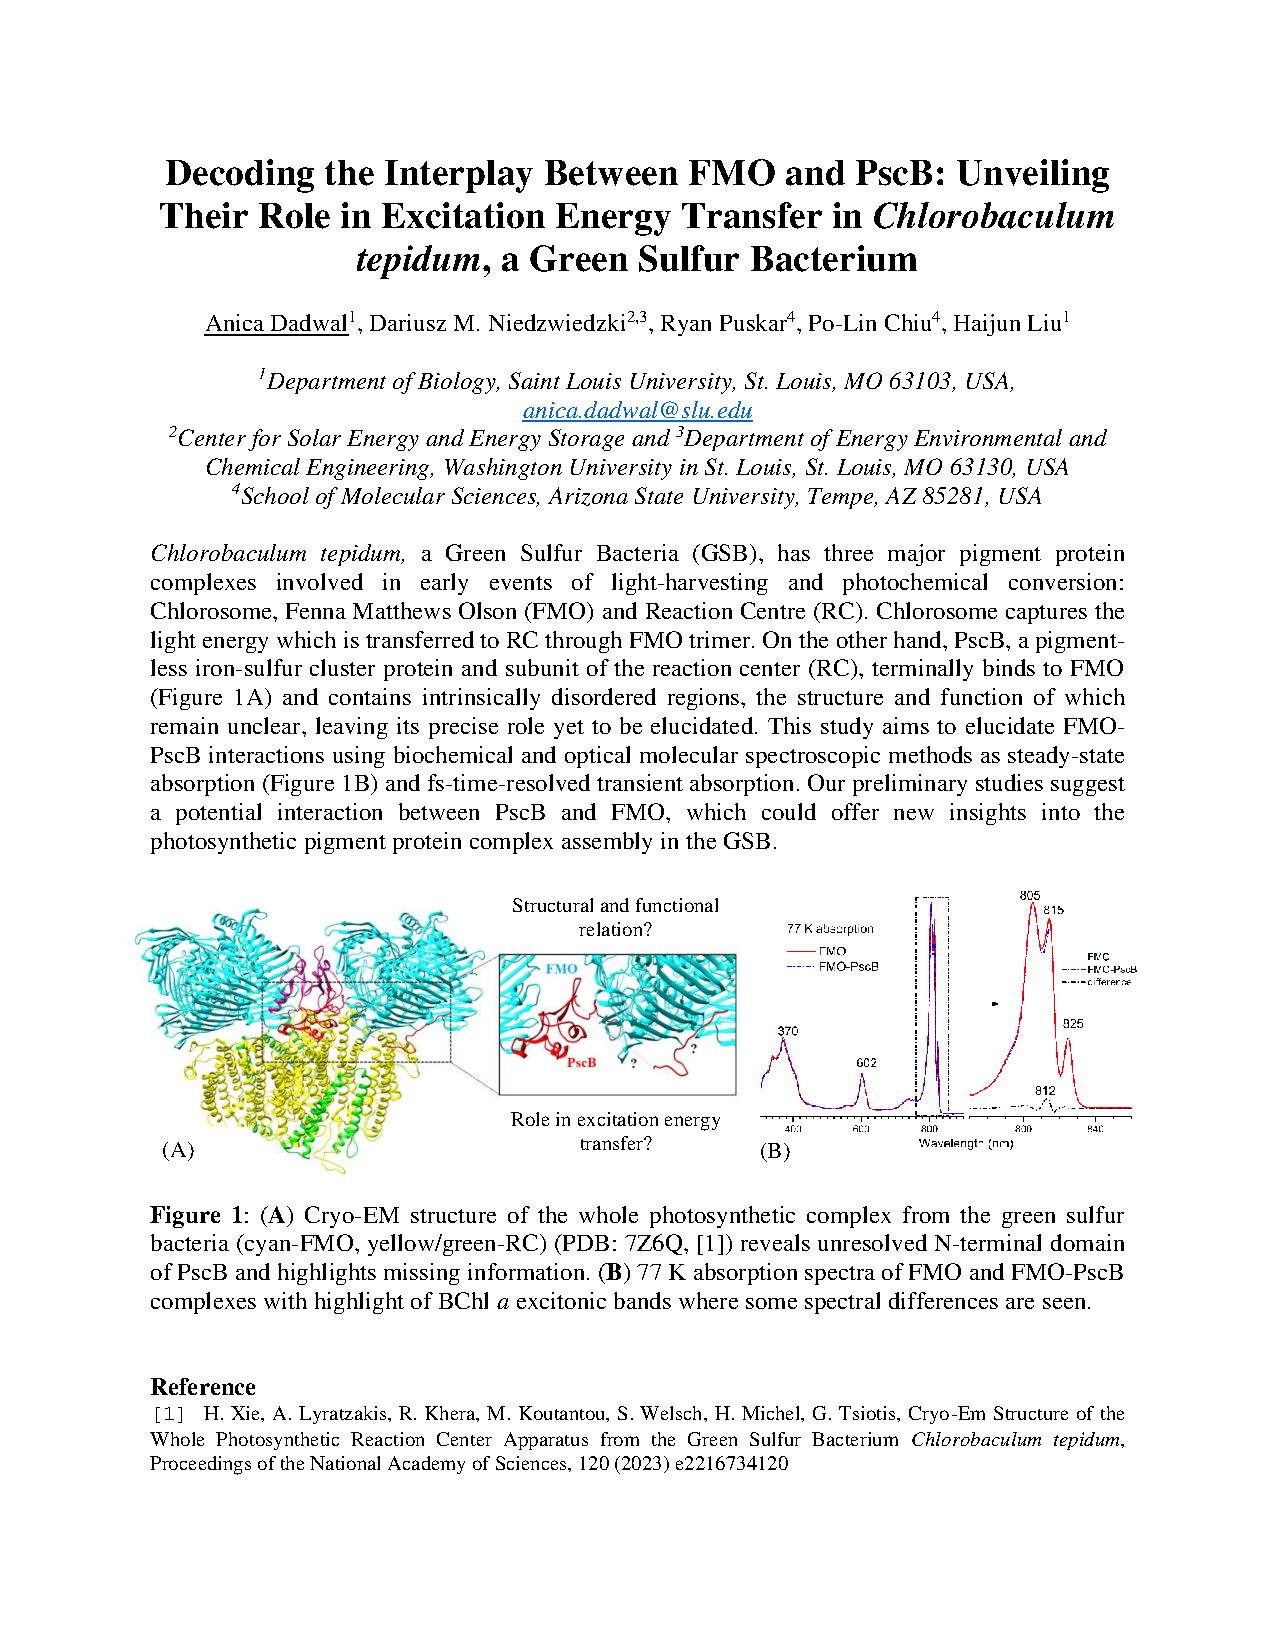
\includepdf[link=true,linkname=Dadwal,pagecommand={\thispagestyle{plain}},addtolist={1,nottalk,heading,abs:Dadwal}]{abstracts/Dadwal_MWSE50.pdf}
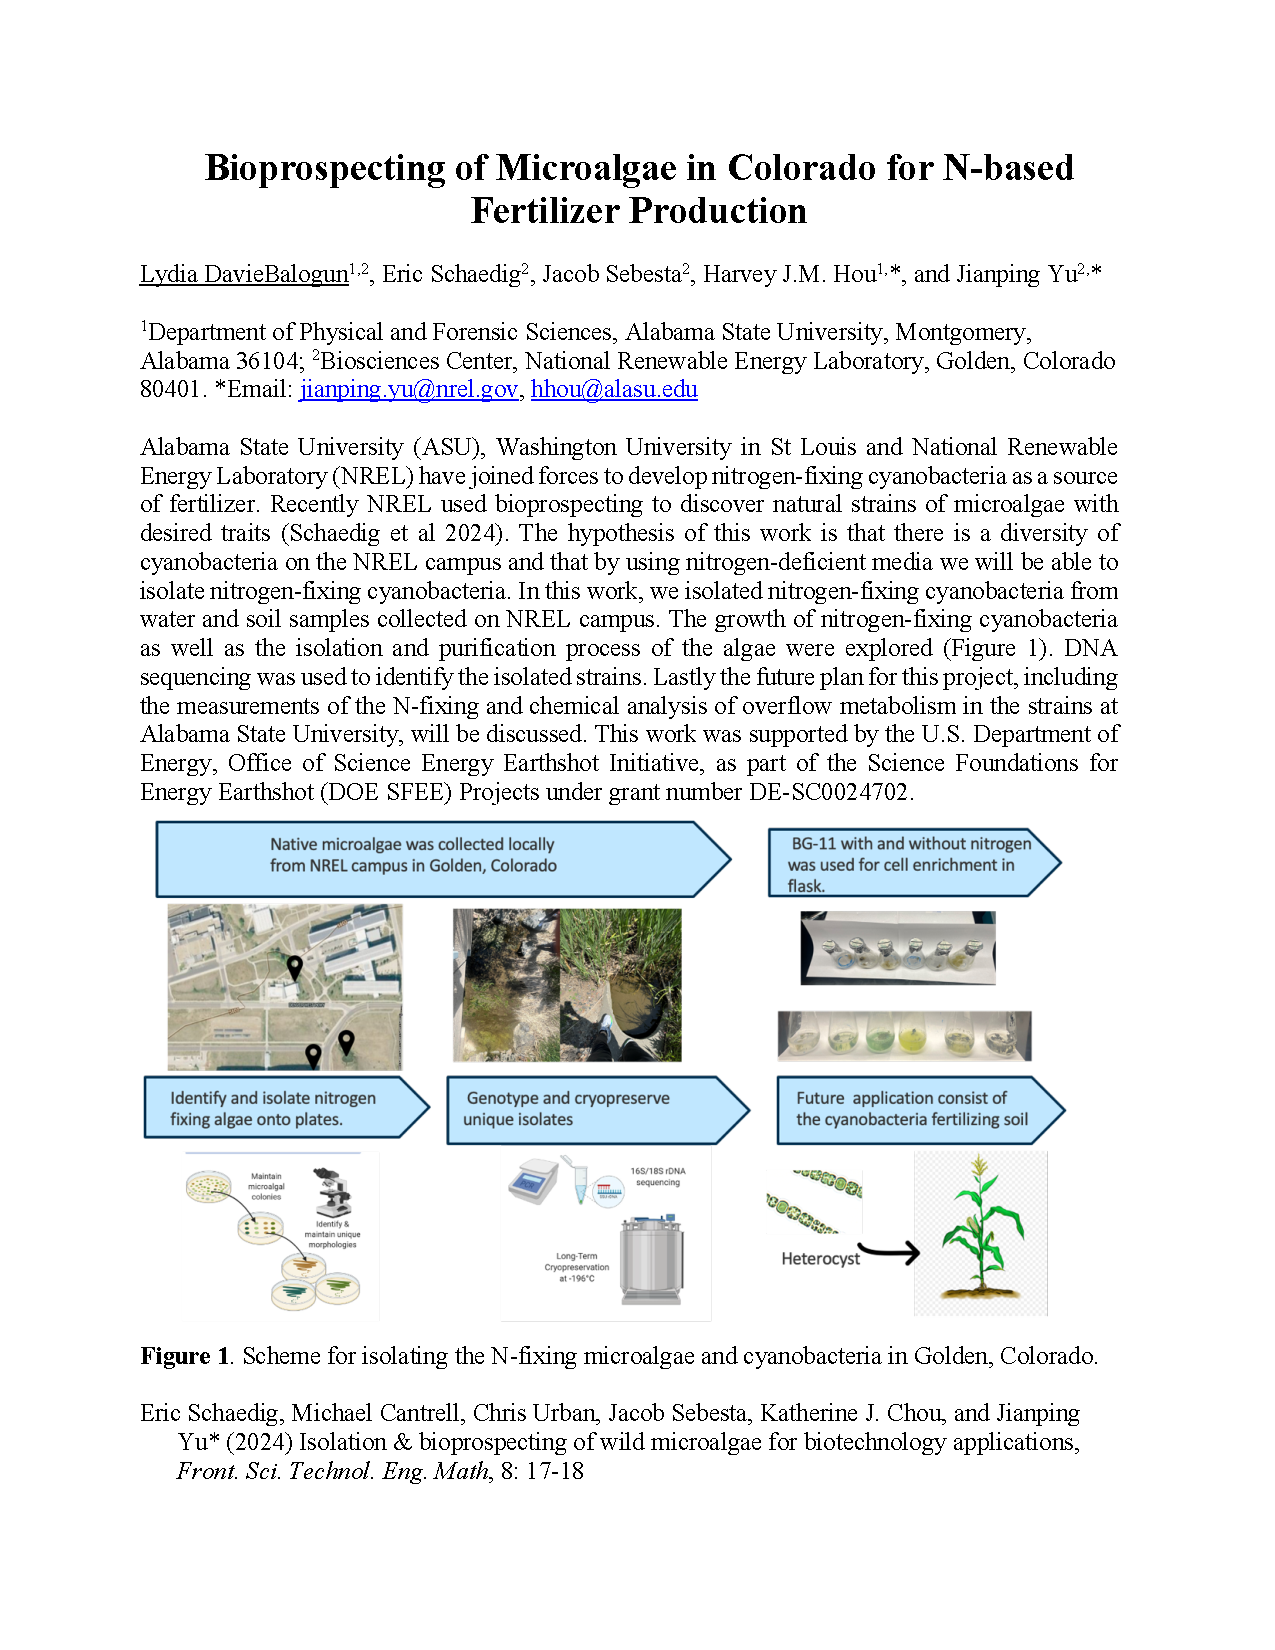
\includepdf[link=true,linkname=Daviebalogun,pagecommand={\thispagestyle{plain}},addtolist={1,nottalk,heading,abs:Daviebalogun}]{abstracts/daviebalogun_MWSE50.pdf}
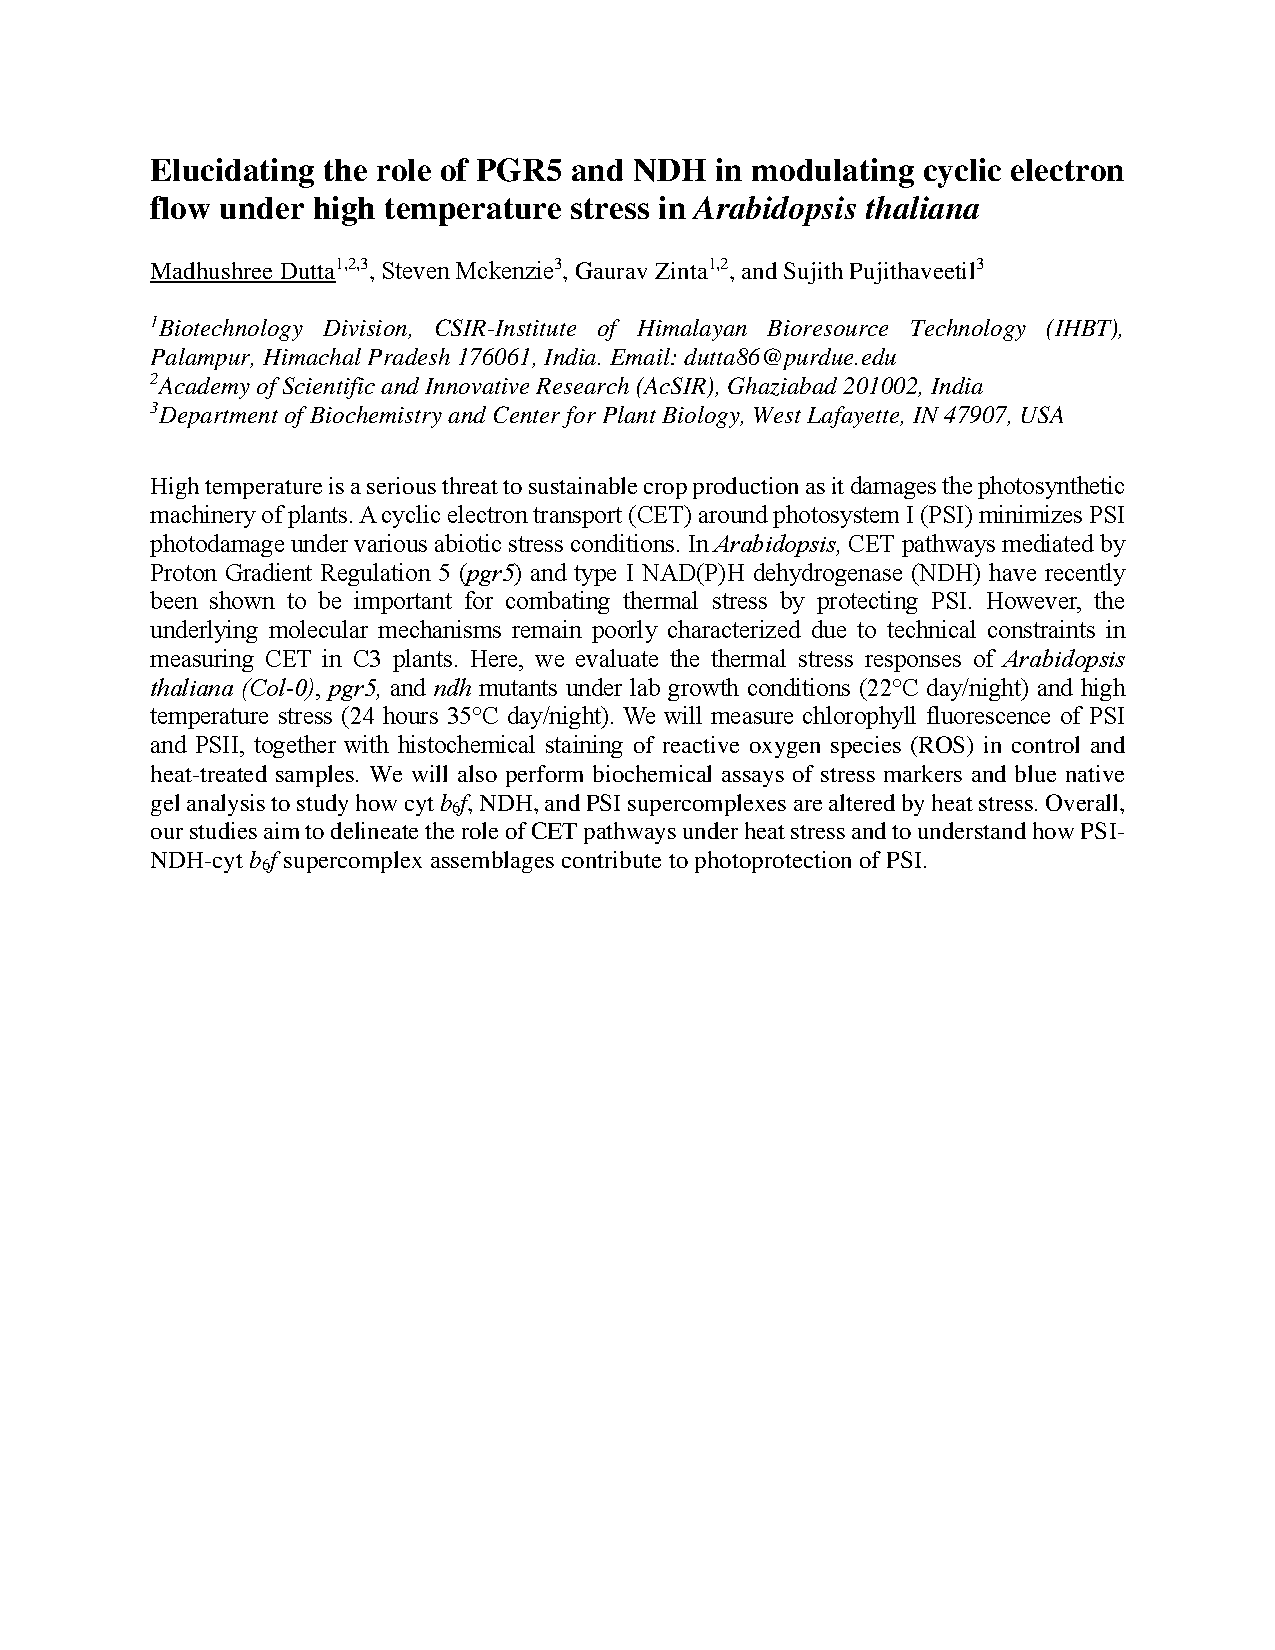
\includepdf[link=true,linkname=Dutta,pagecommand={\thispagestyle{plain}},addtolist={1,nottalk,heading,abs:Dutta}]{abstracts/Dutta_MWSE50.pdf}
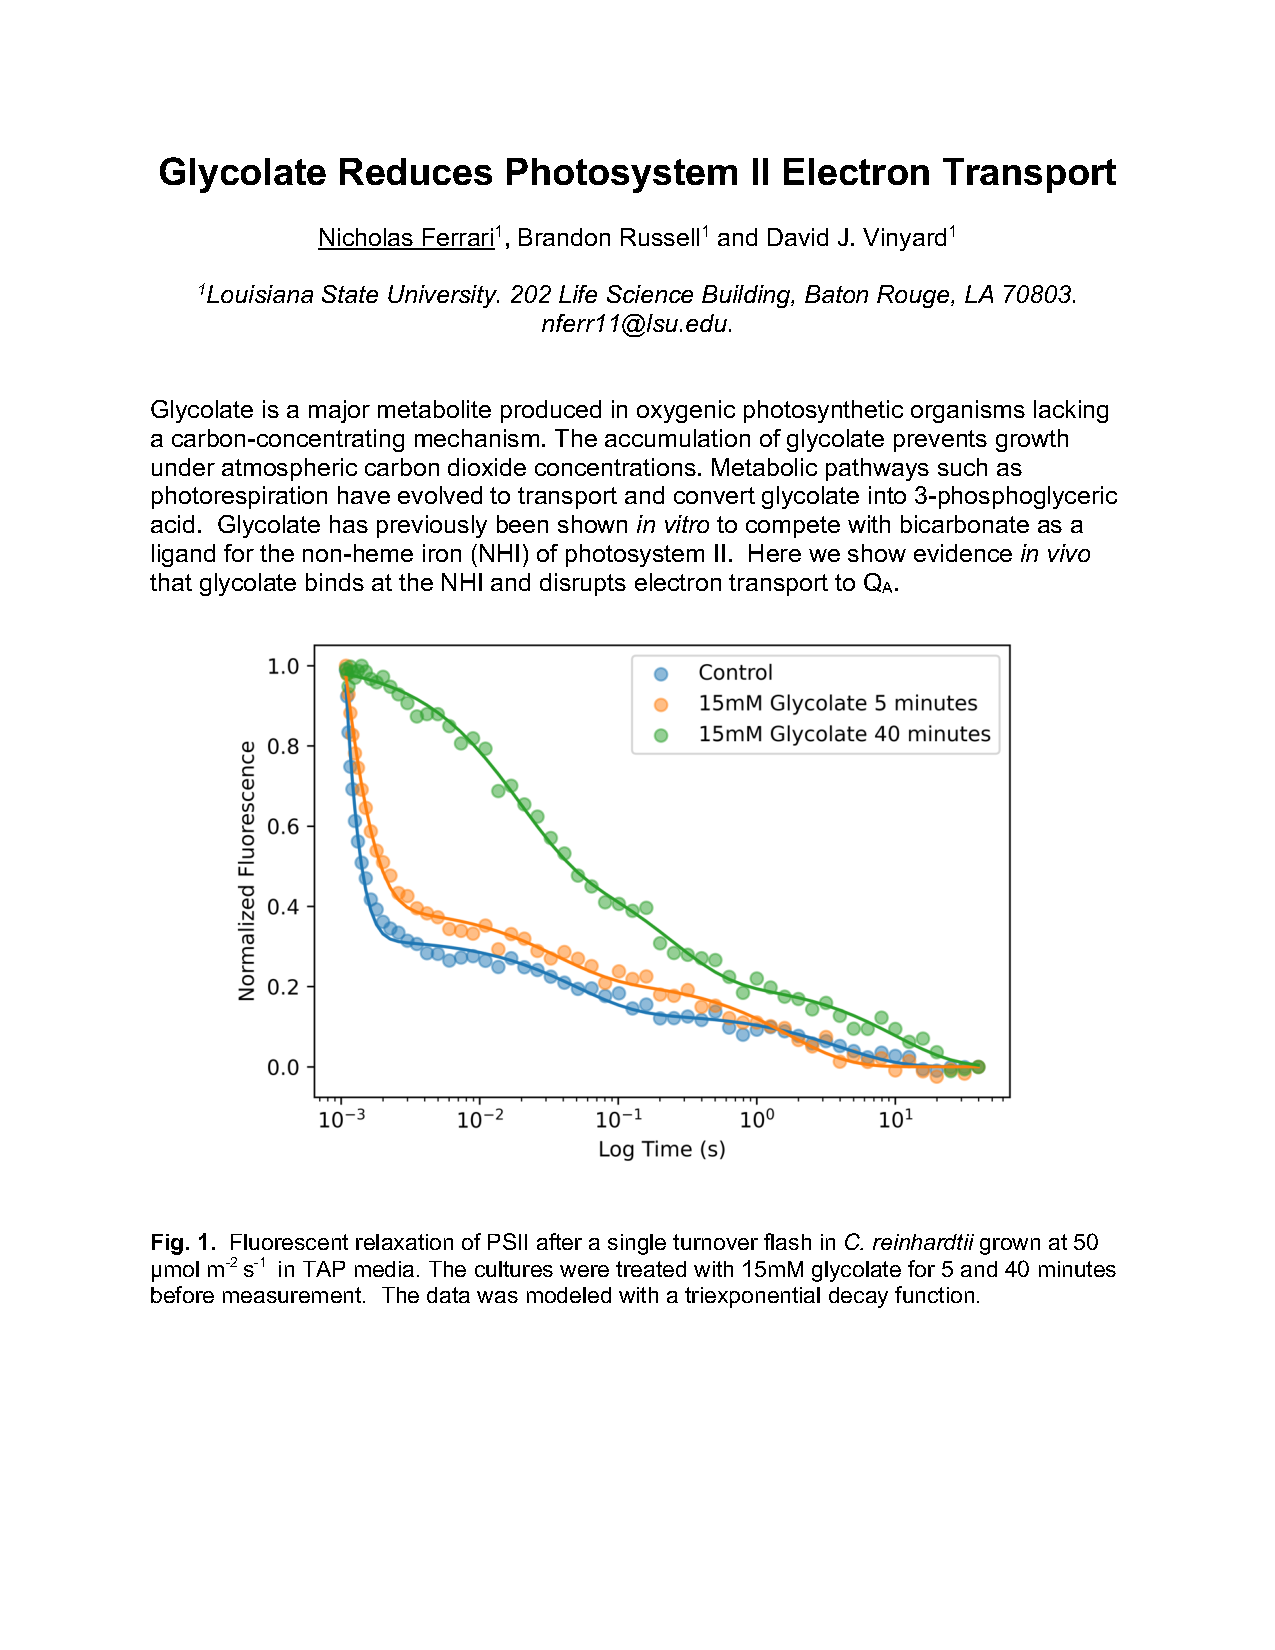
\includepdf[link=true,linkname=Ferrari,pagecommand={\thispagestyle{plain}},addtolist={1,nottalk,heading,abs:Ferrari}]{abstracts/Ferrari_MWSE50.pdf}
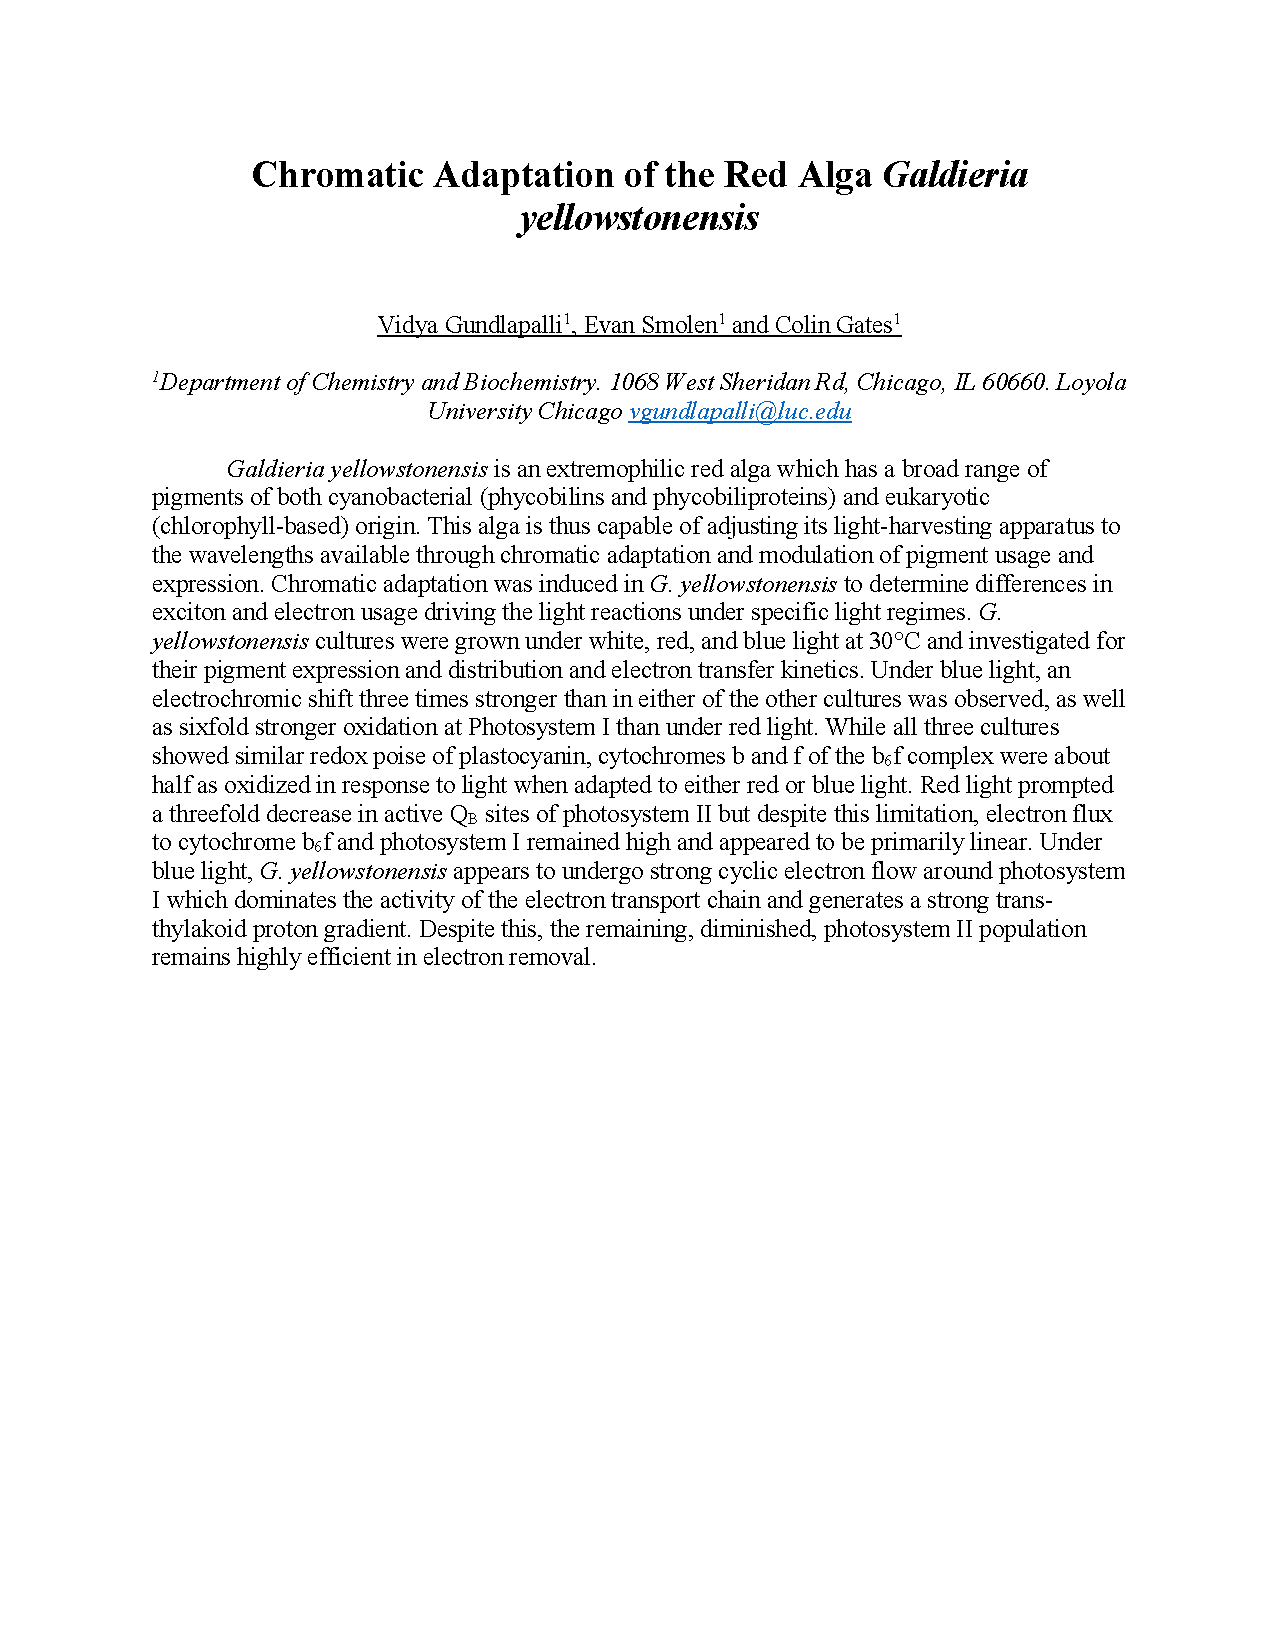
\includepdf[link=true,linkname=Gundlapalli,pagecommand={\thispagestyle{plain}},addtolist={1,nottalk,heading,abs:Gundlapalli}]{abstracts/Gundlapalli_MWSE50.pdf}
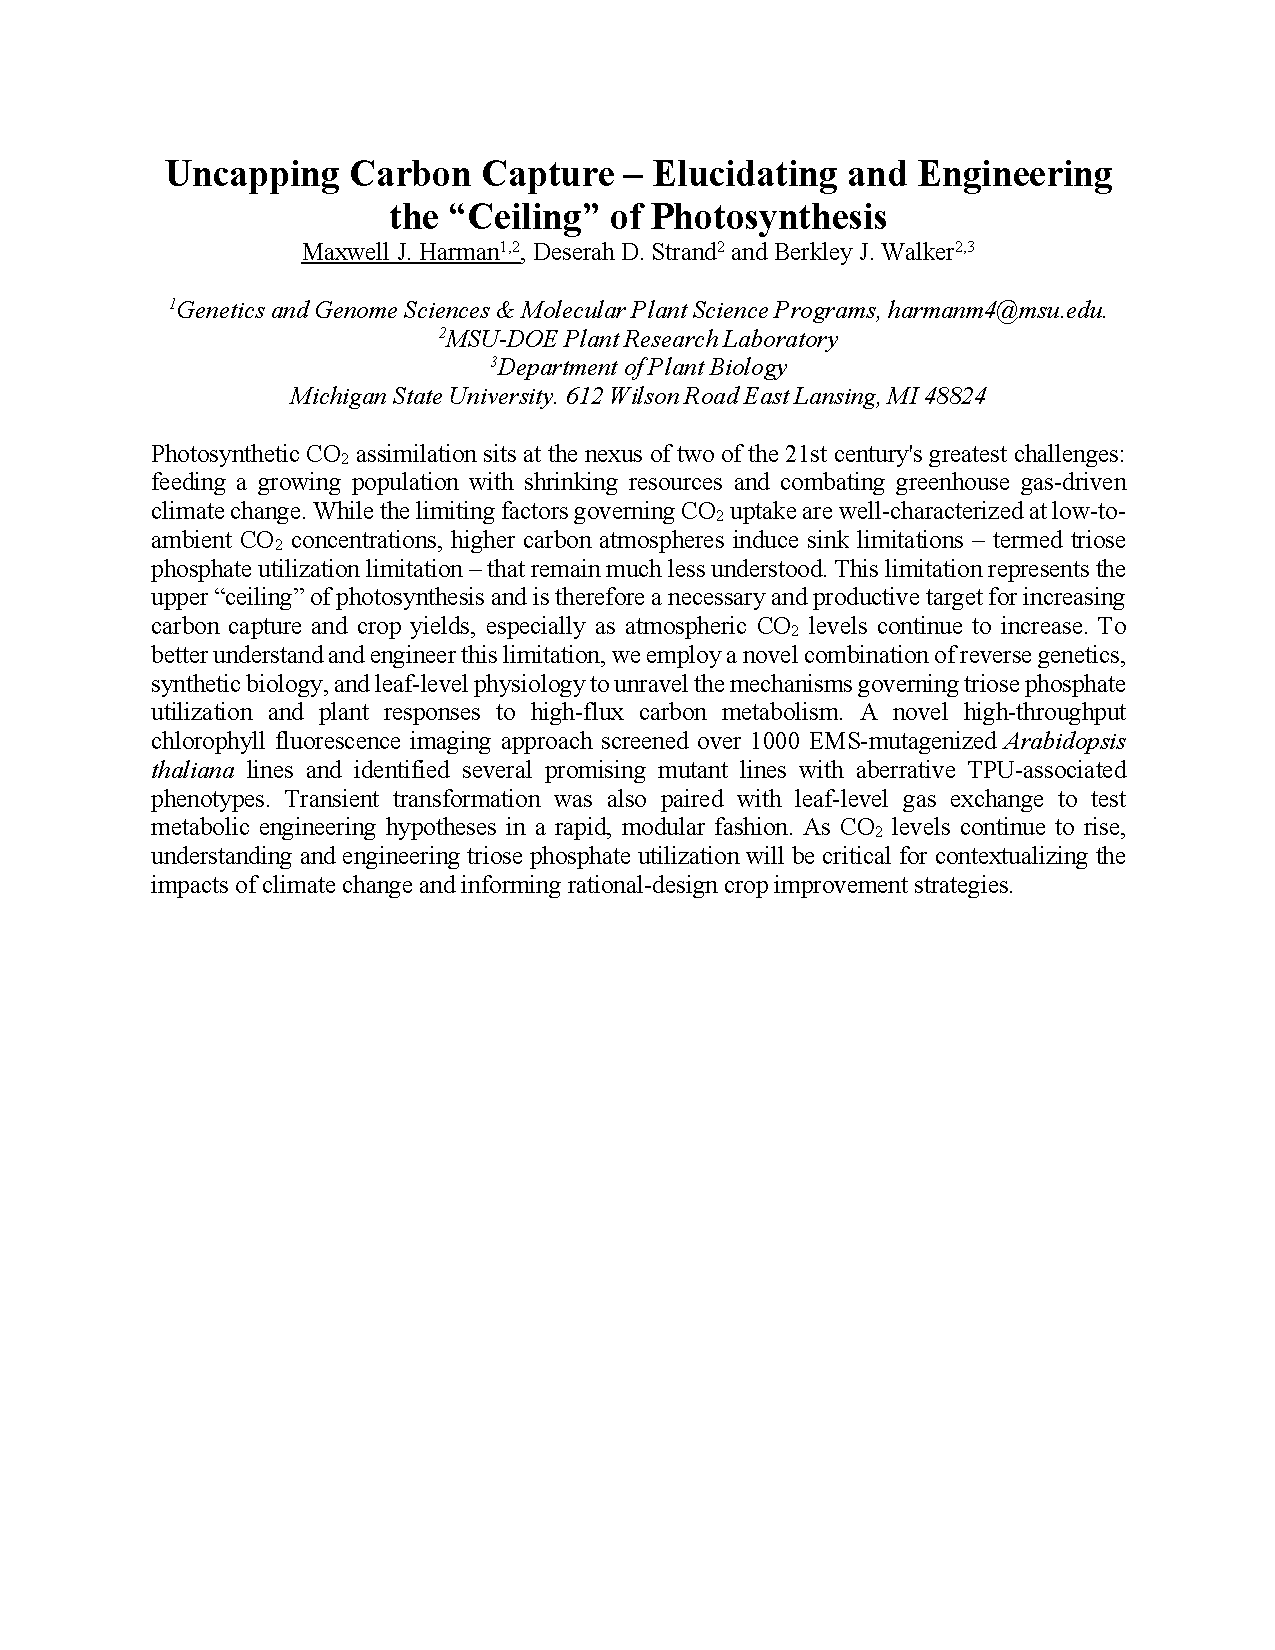
\includepdf[link=true,linkname=Harman,pagecommand={\thispagestyle{plain}},addtolist={1,nottalk,heading,abs:Harman}]{abstracts/Harman_MWSE50.pdf}
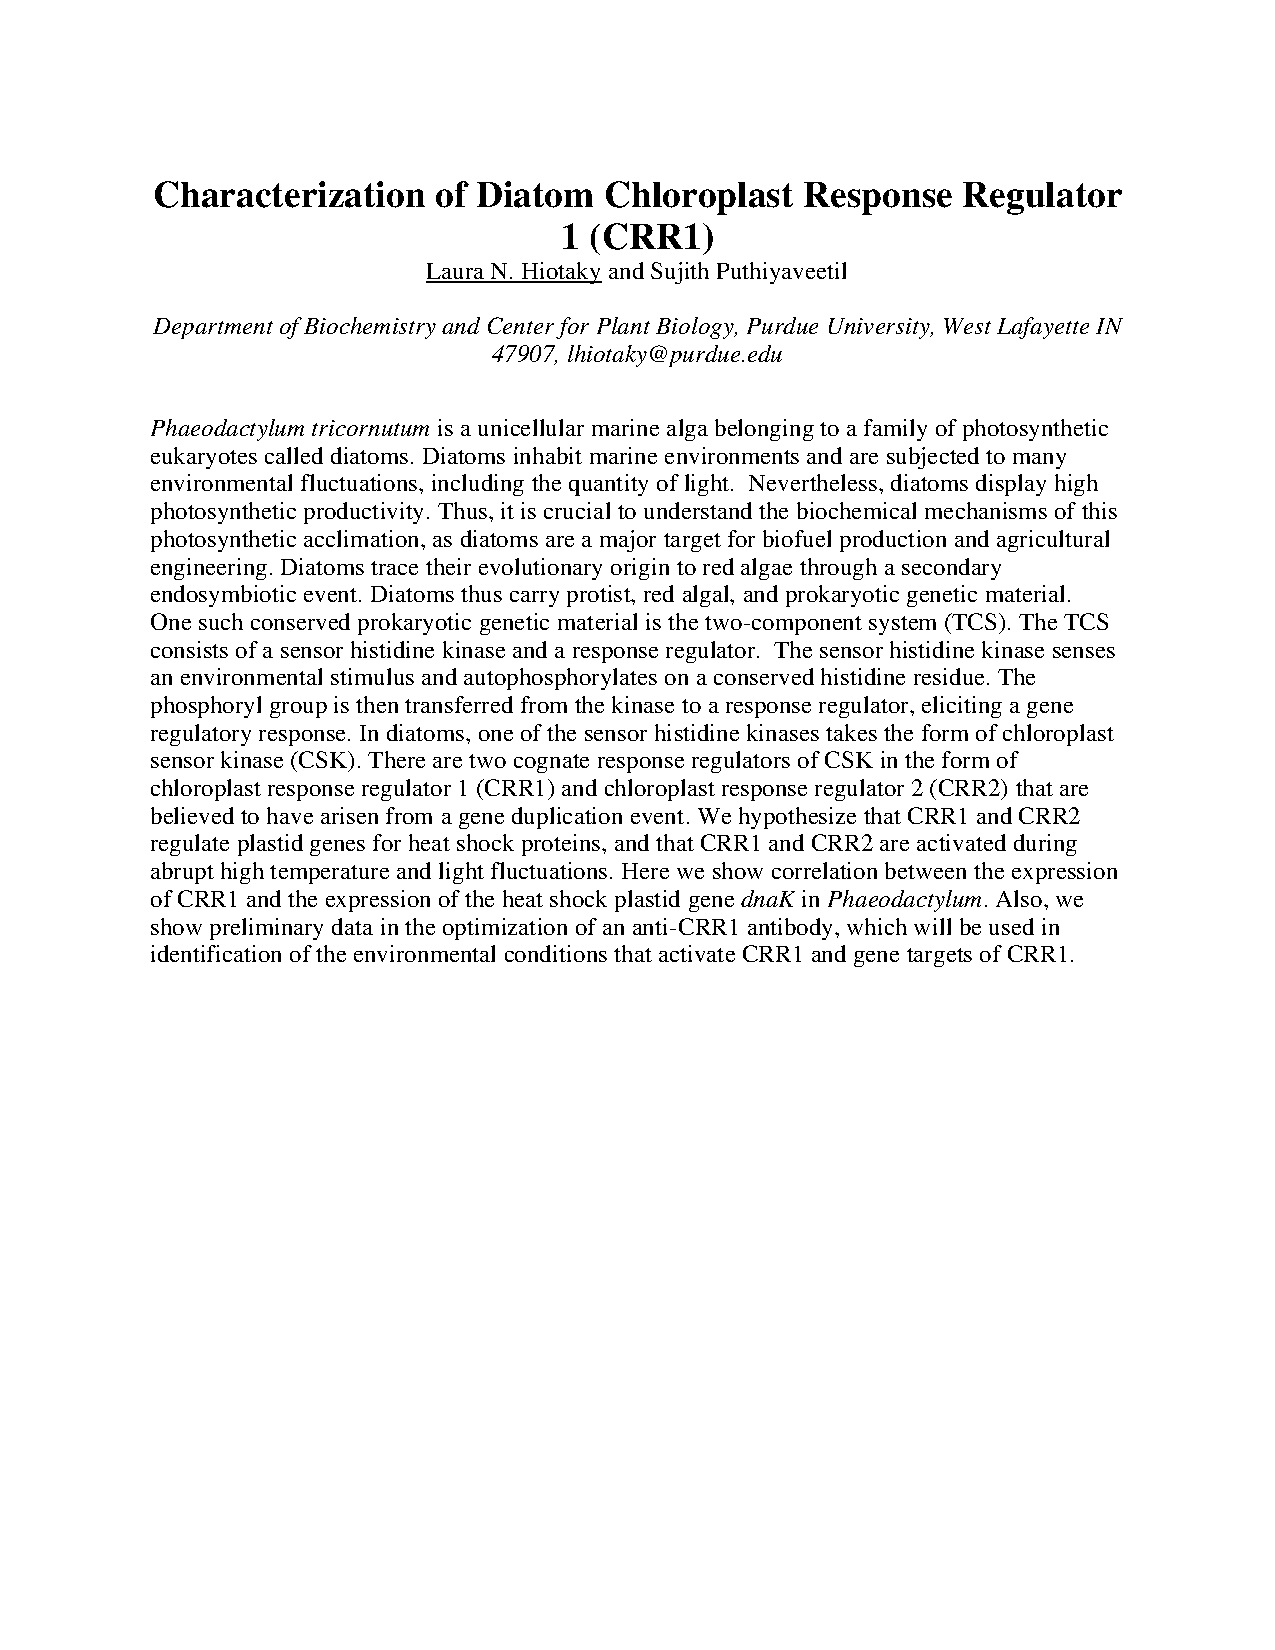
\includepdf[link=true,linkname=Hiotaky,pagecommand={\thispagestyle{plain}},addtolist={1,nottalk,heading,abs:Hiotaky}]{abstracts/Hiotaky_MWSE50.pdf}
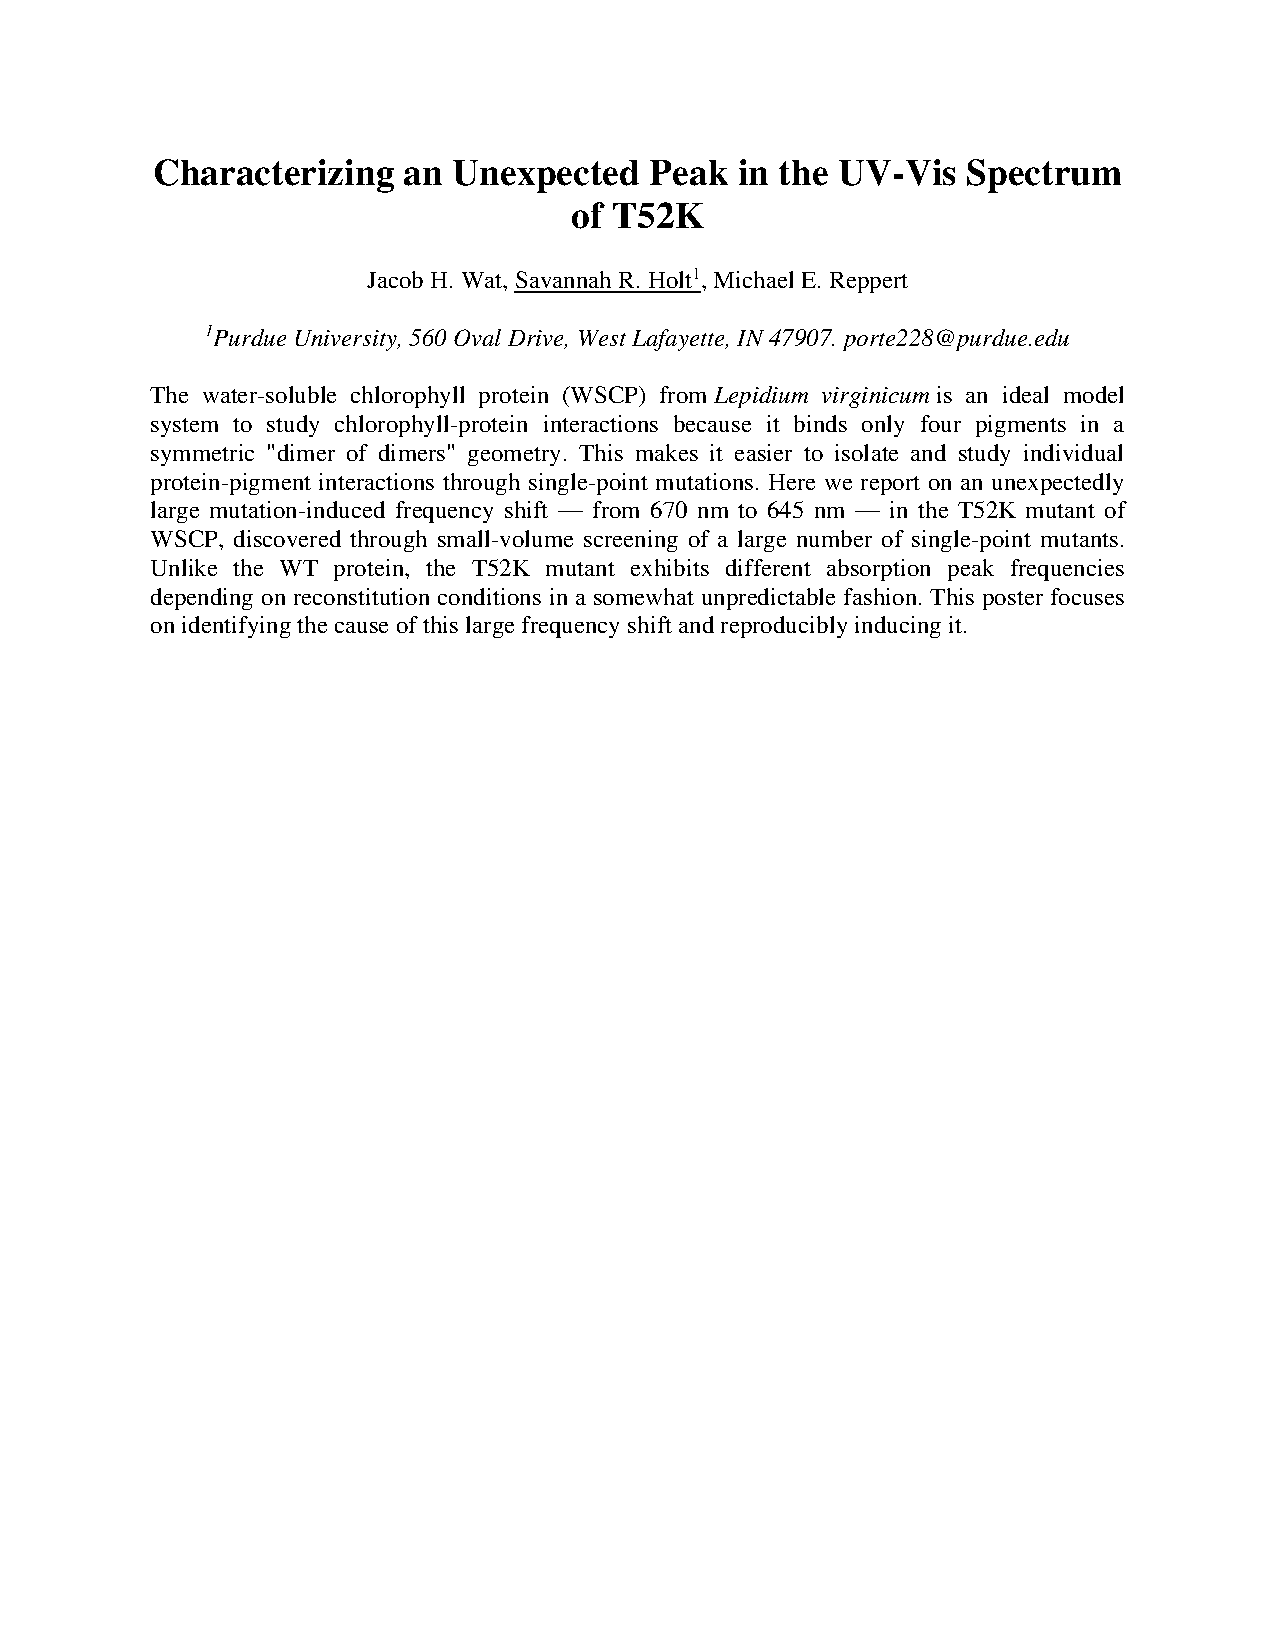
\includepdf[link=true,linkname=Holt,pagecommand={\thispagestyle{plain}},addtolist={1,nottalk,heading,abs:Holt}]{abstracts/Holt_MWSE50.pdf}
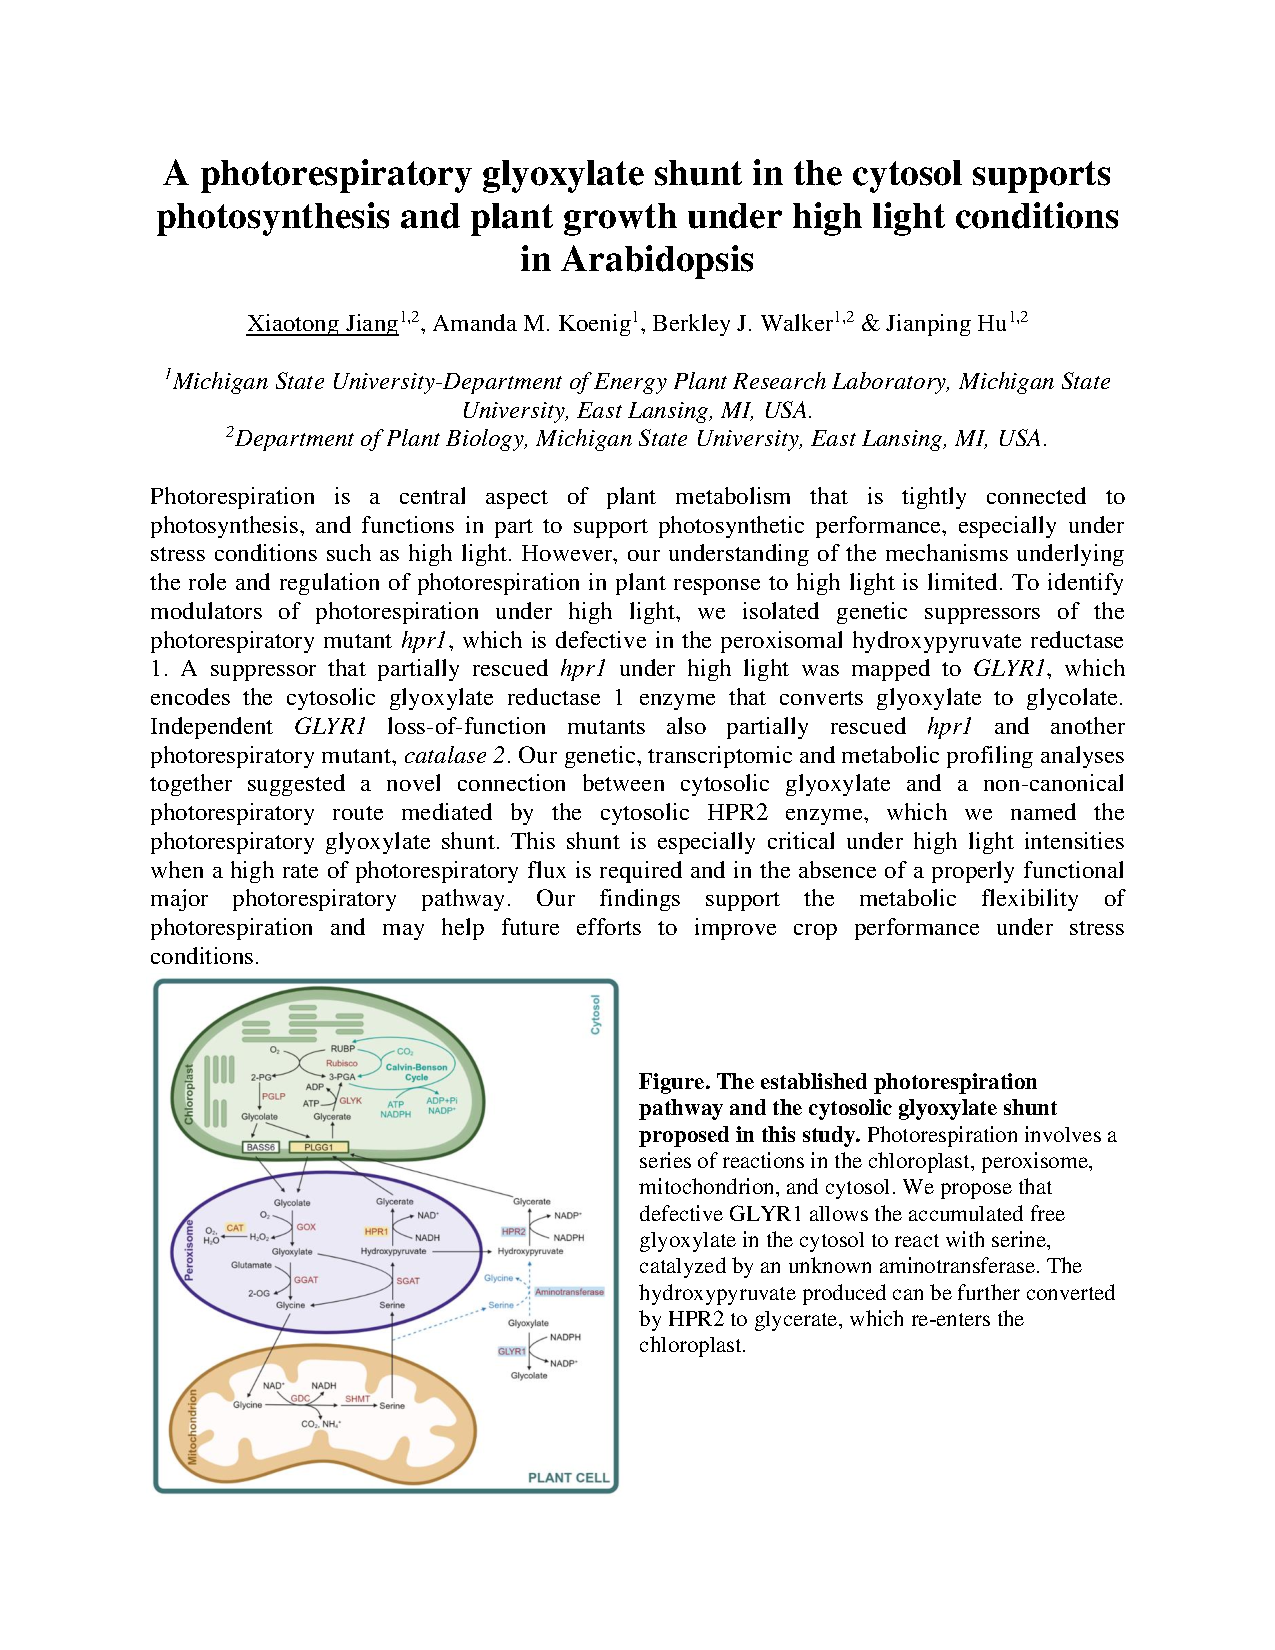
\includepdf[link=true,linkname=Jiang,pagecommand={\thispagestyle{plain}},addtolist={1,nottalk,heading,abs:Jiang}]{abstracts/Jiang_MWSE50.pdf}
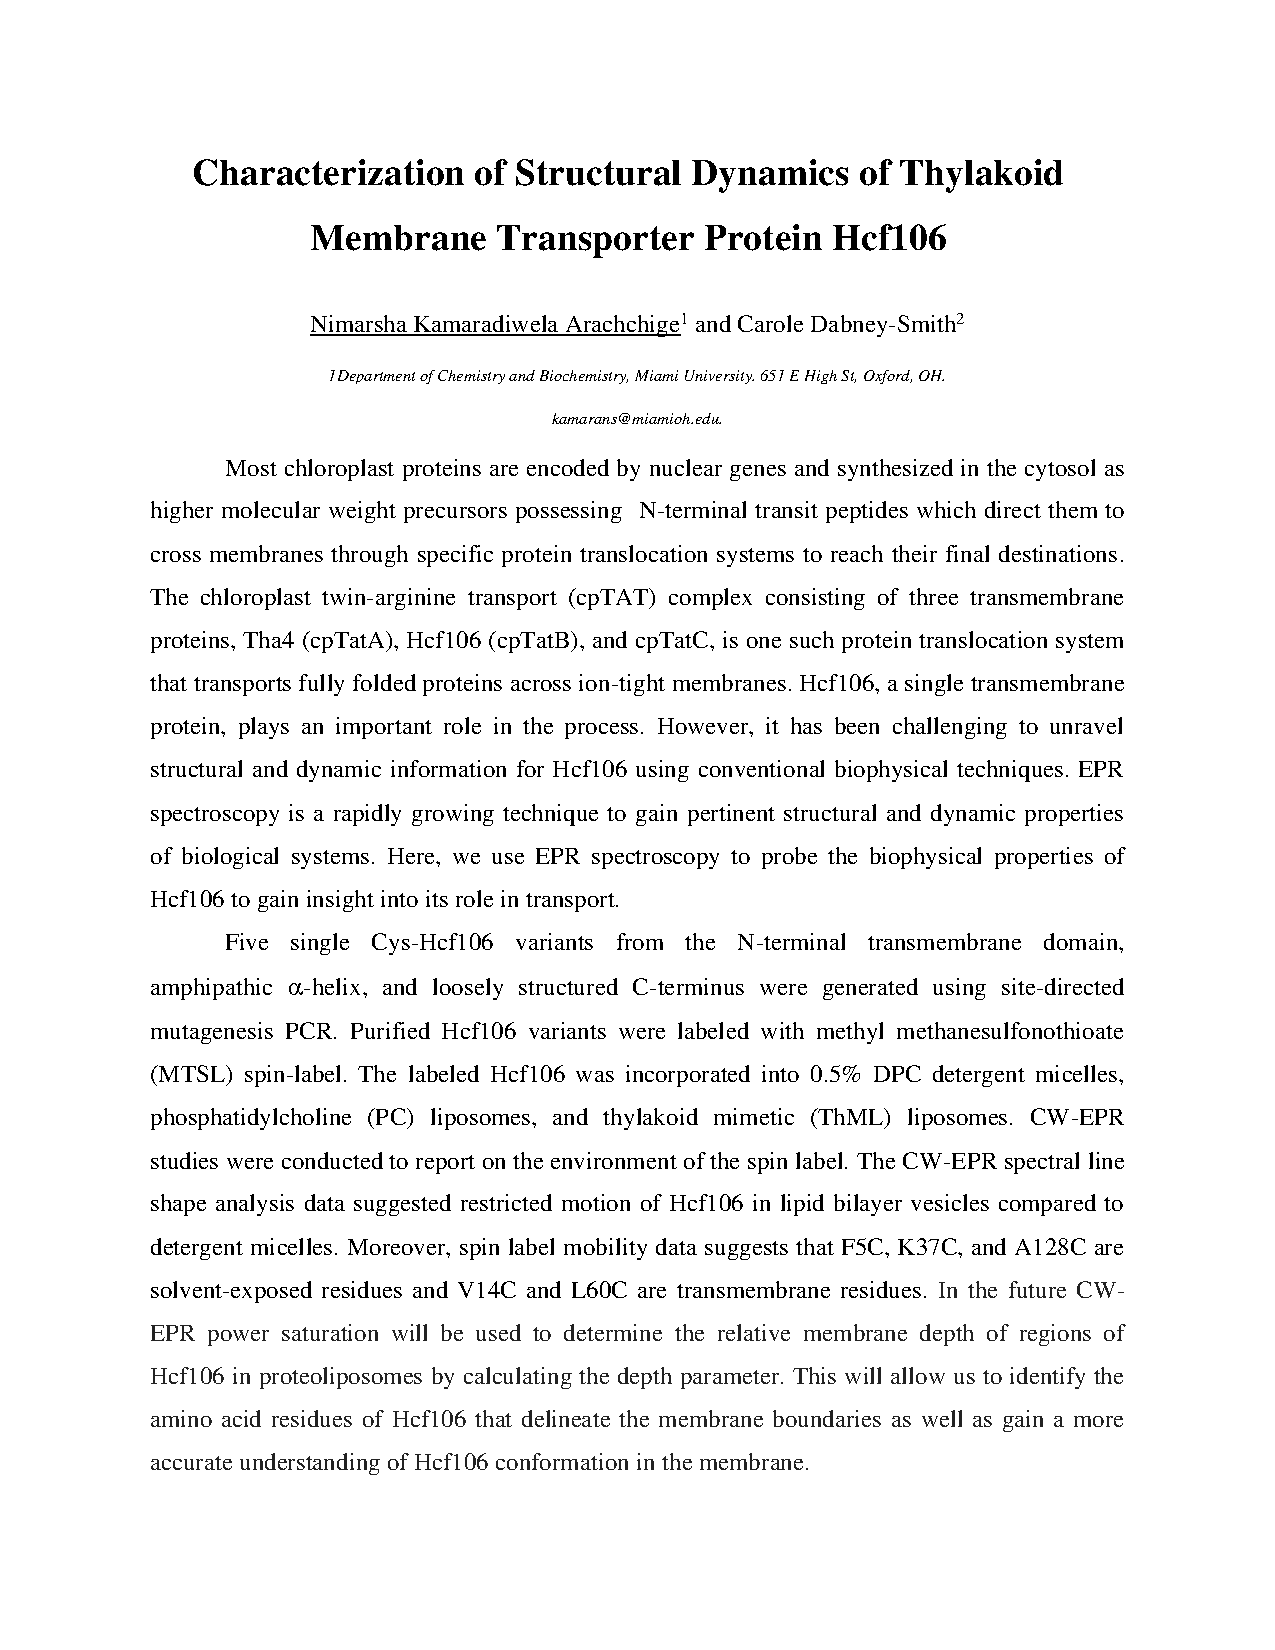
\includepdf[link=true,linkname=Kamaradiwelaarachchige,pagecommand={\thispagestyle{plain}},addtolist={1,nottalk,heading,abs:Kamaradiwelaarachchige}]{abstracts/KamaradiwelaArachchige_MWSE50.pdf}
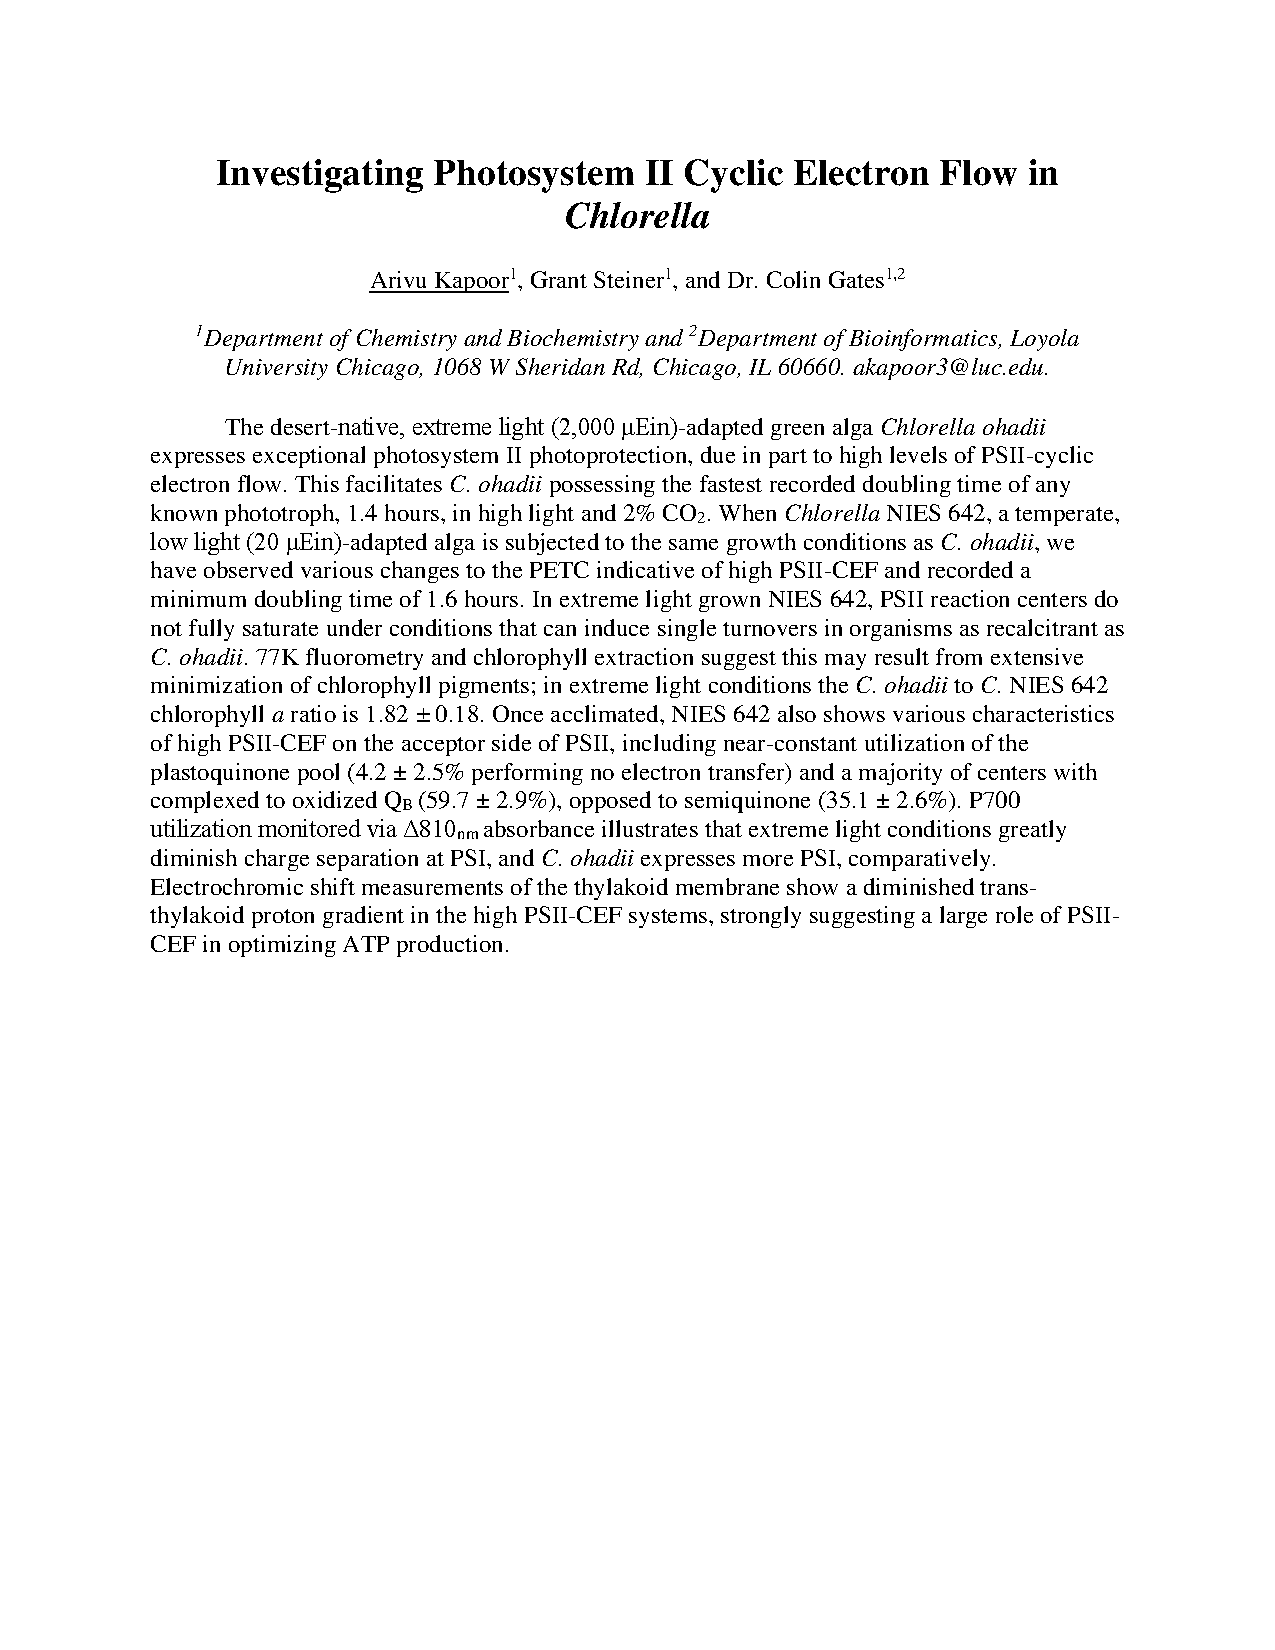
\includepdf[link=true,linkname=Kapoor,pagecommand={\thispagestyle{plain}},addtolist={1,nottalk,heading,abs:Kapoor}]{abstracts/Kapoor_MWSE50.pdf}
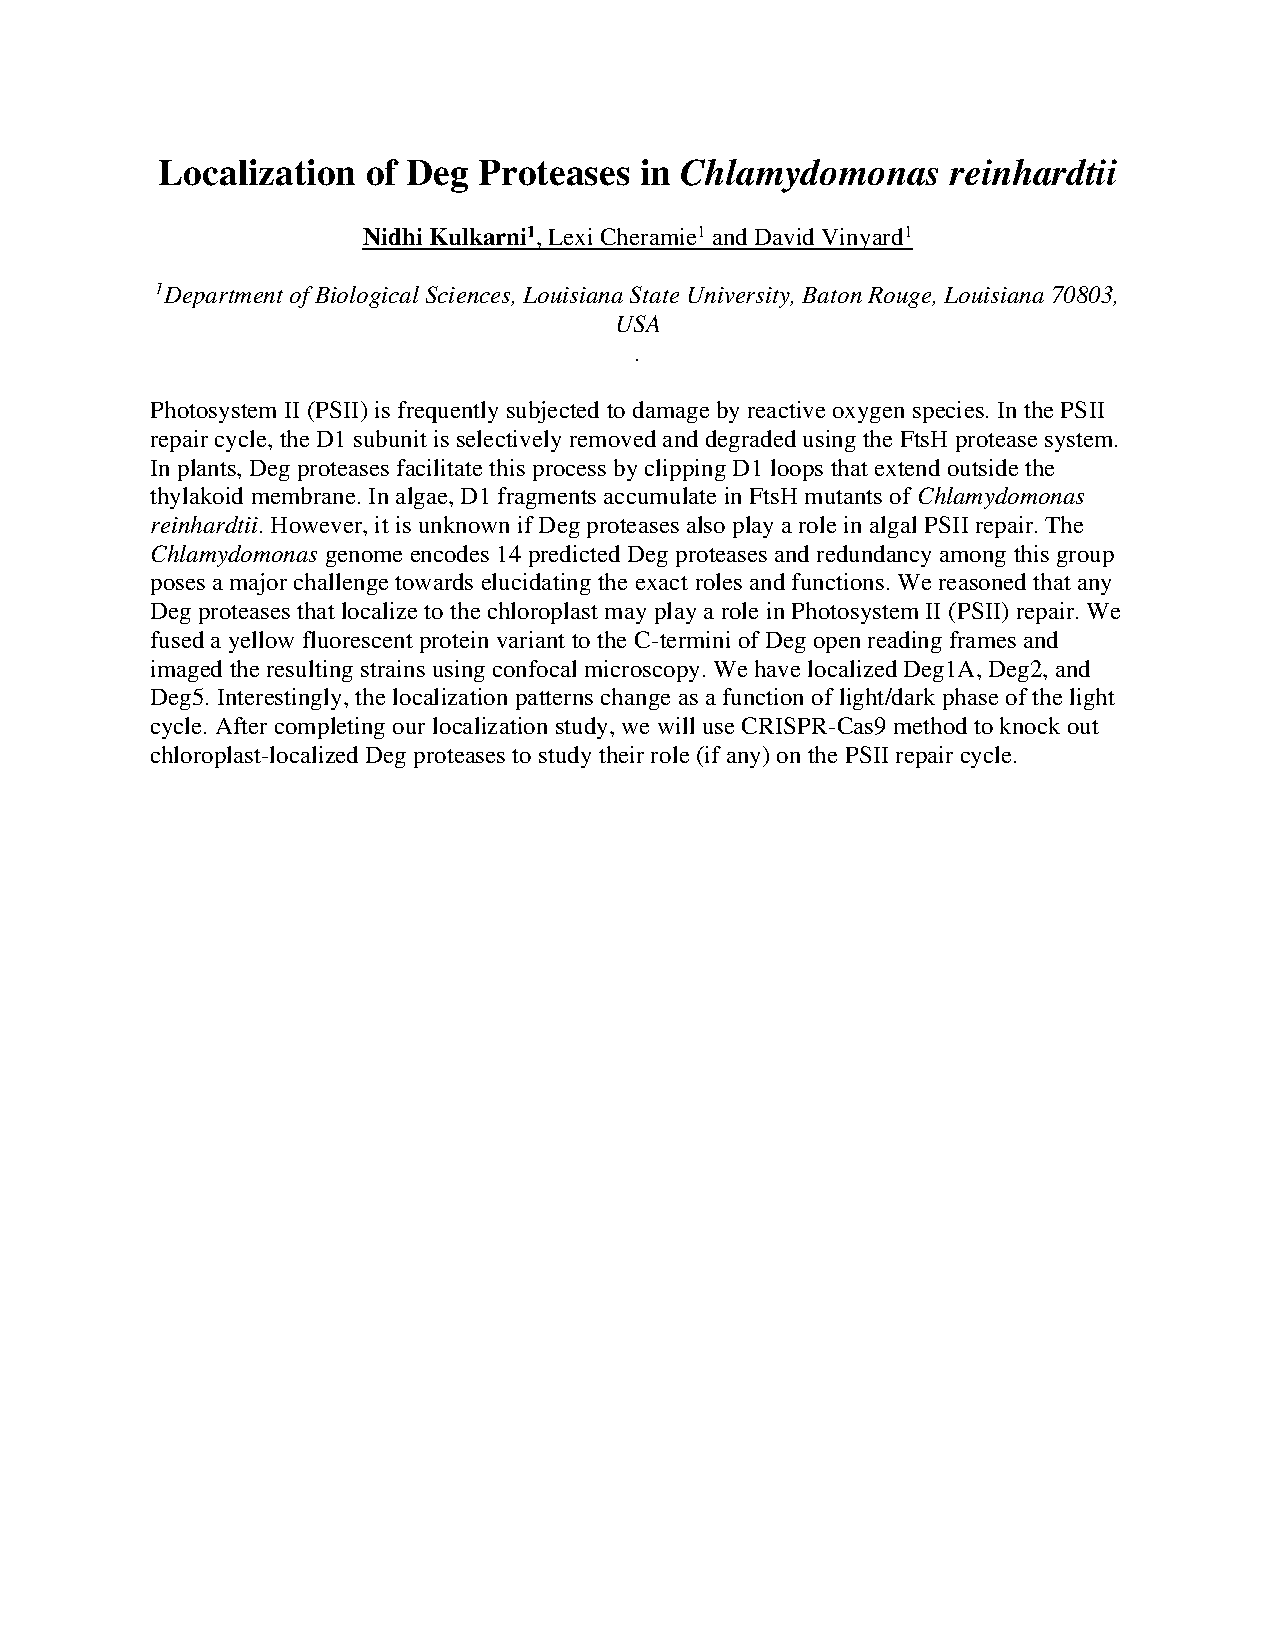
\includepdf[link=true,linkname=Kulkarni,pagecommand={\thispagestyle{plain}},addtolist={1,nottalk,heading,abs:Kulkarni}]{abstracts/Kulkarni_MWSE50.pdf}
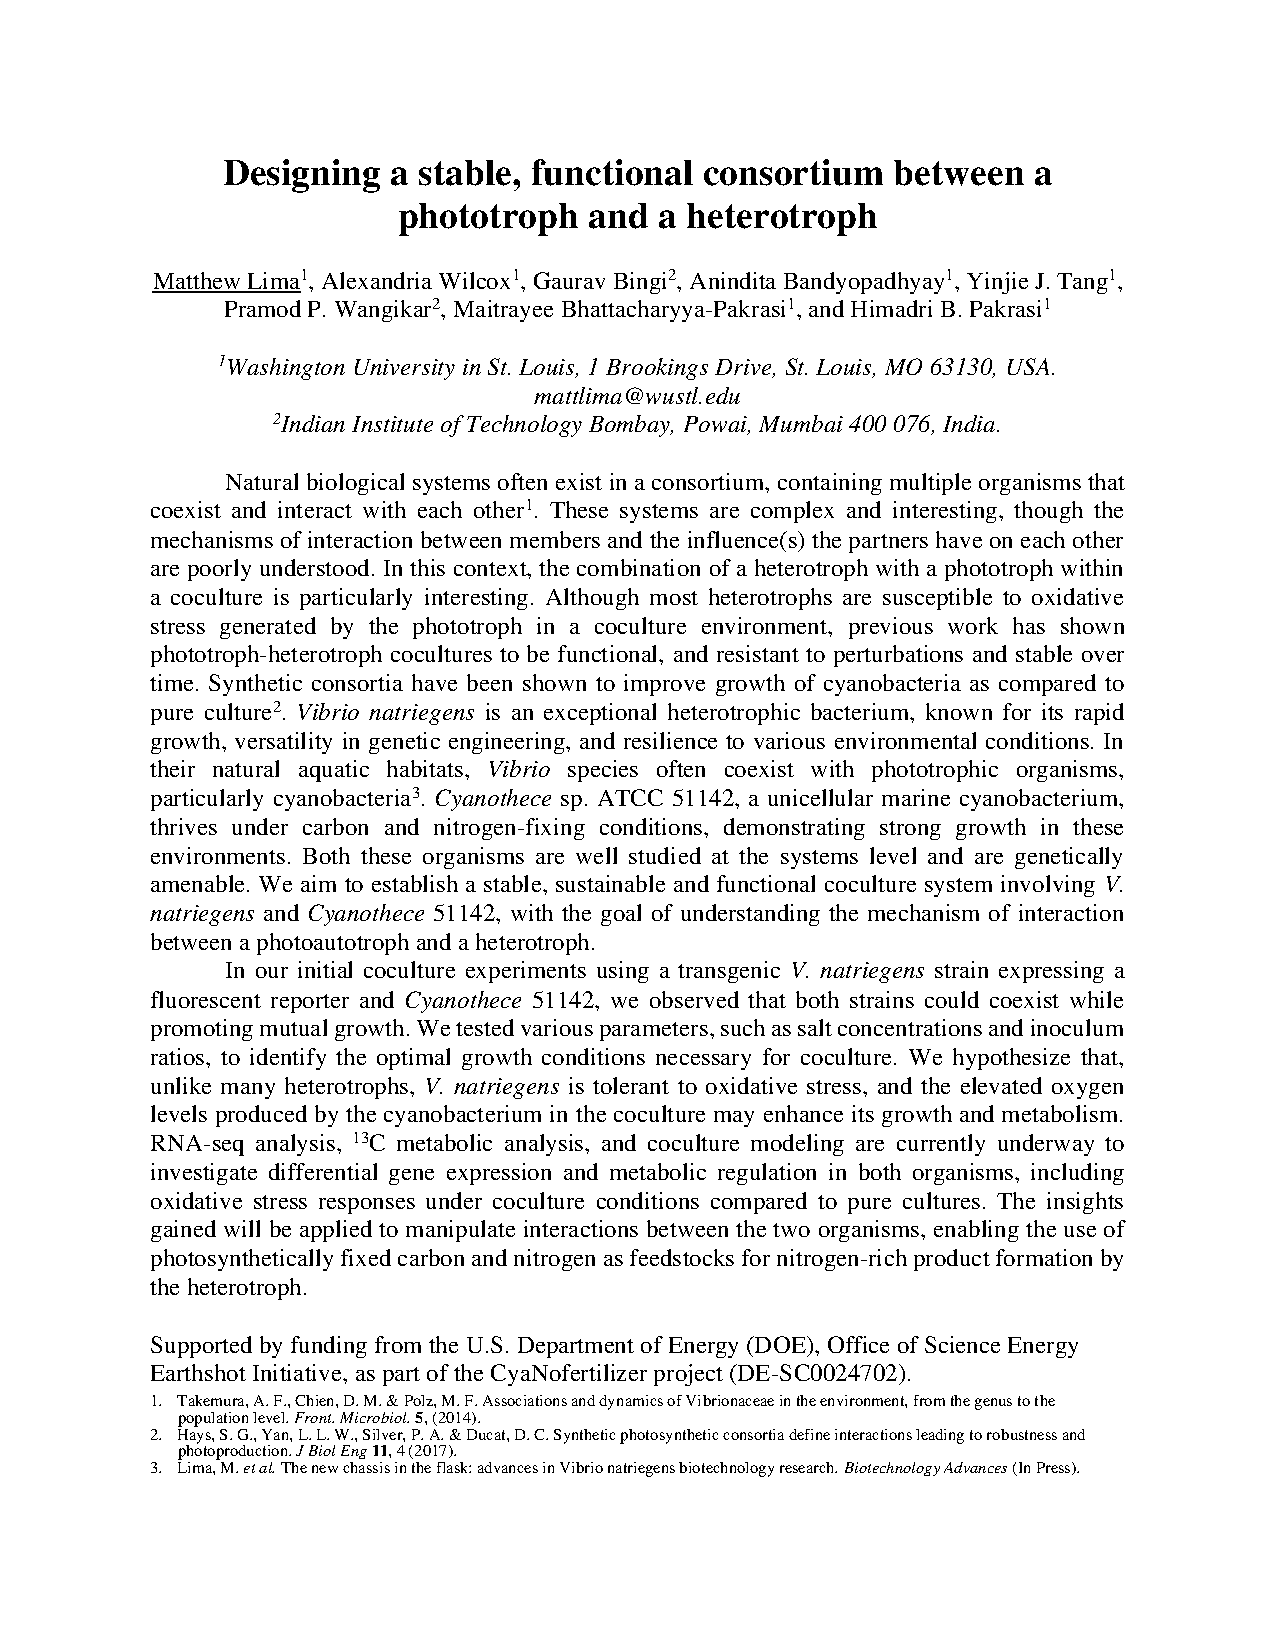
\includepdf[link=true,linkname=Lima,pagecommand={\thispagestyle{plain}},addtolist={1,nottalk,heading,abs:Lima}]{abstracts/Lima_MWSE50.pdf}
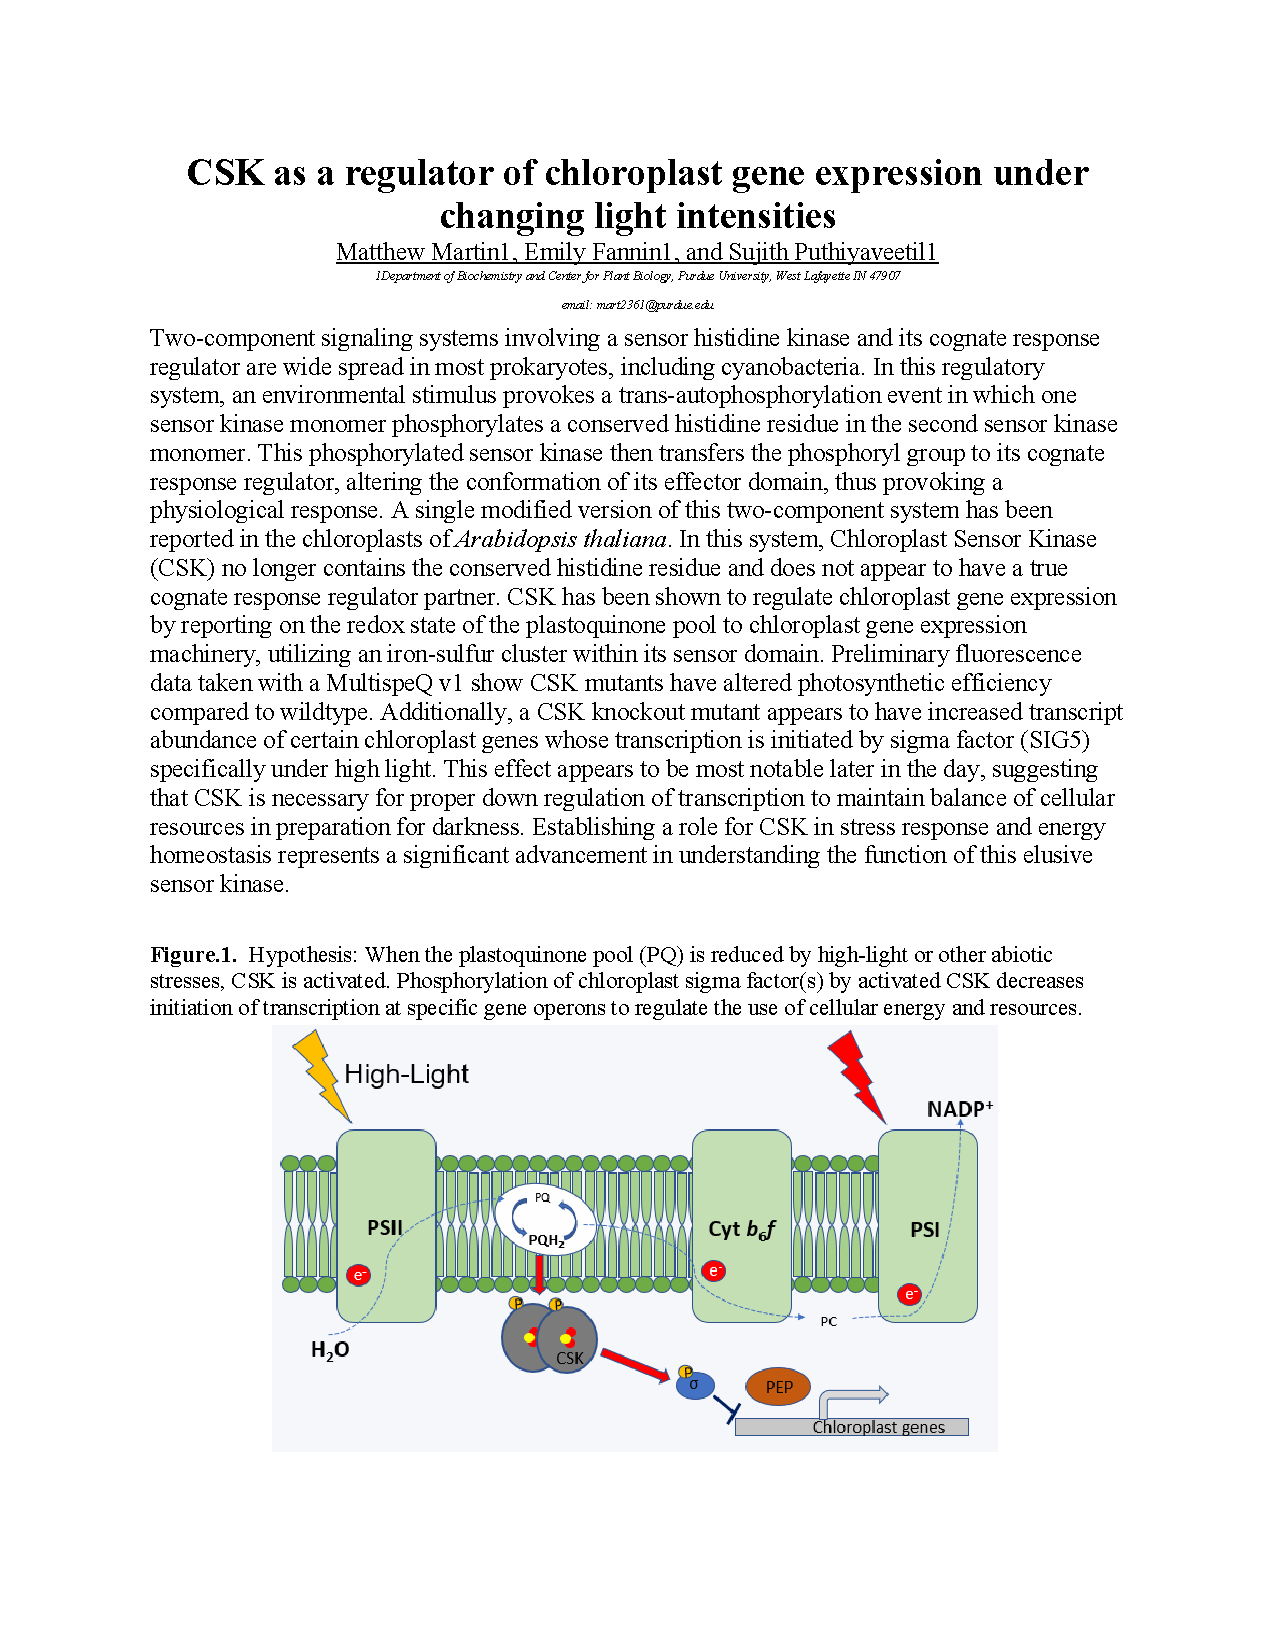
\includepdf[link=true,linkname=Martin,pagecommand={\thispagestyle{plain}},addtolist={1,nottalk,heading,abs:Martin}]{abstracts/Martin_MWSE50.pdf}
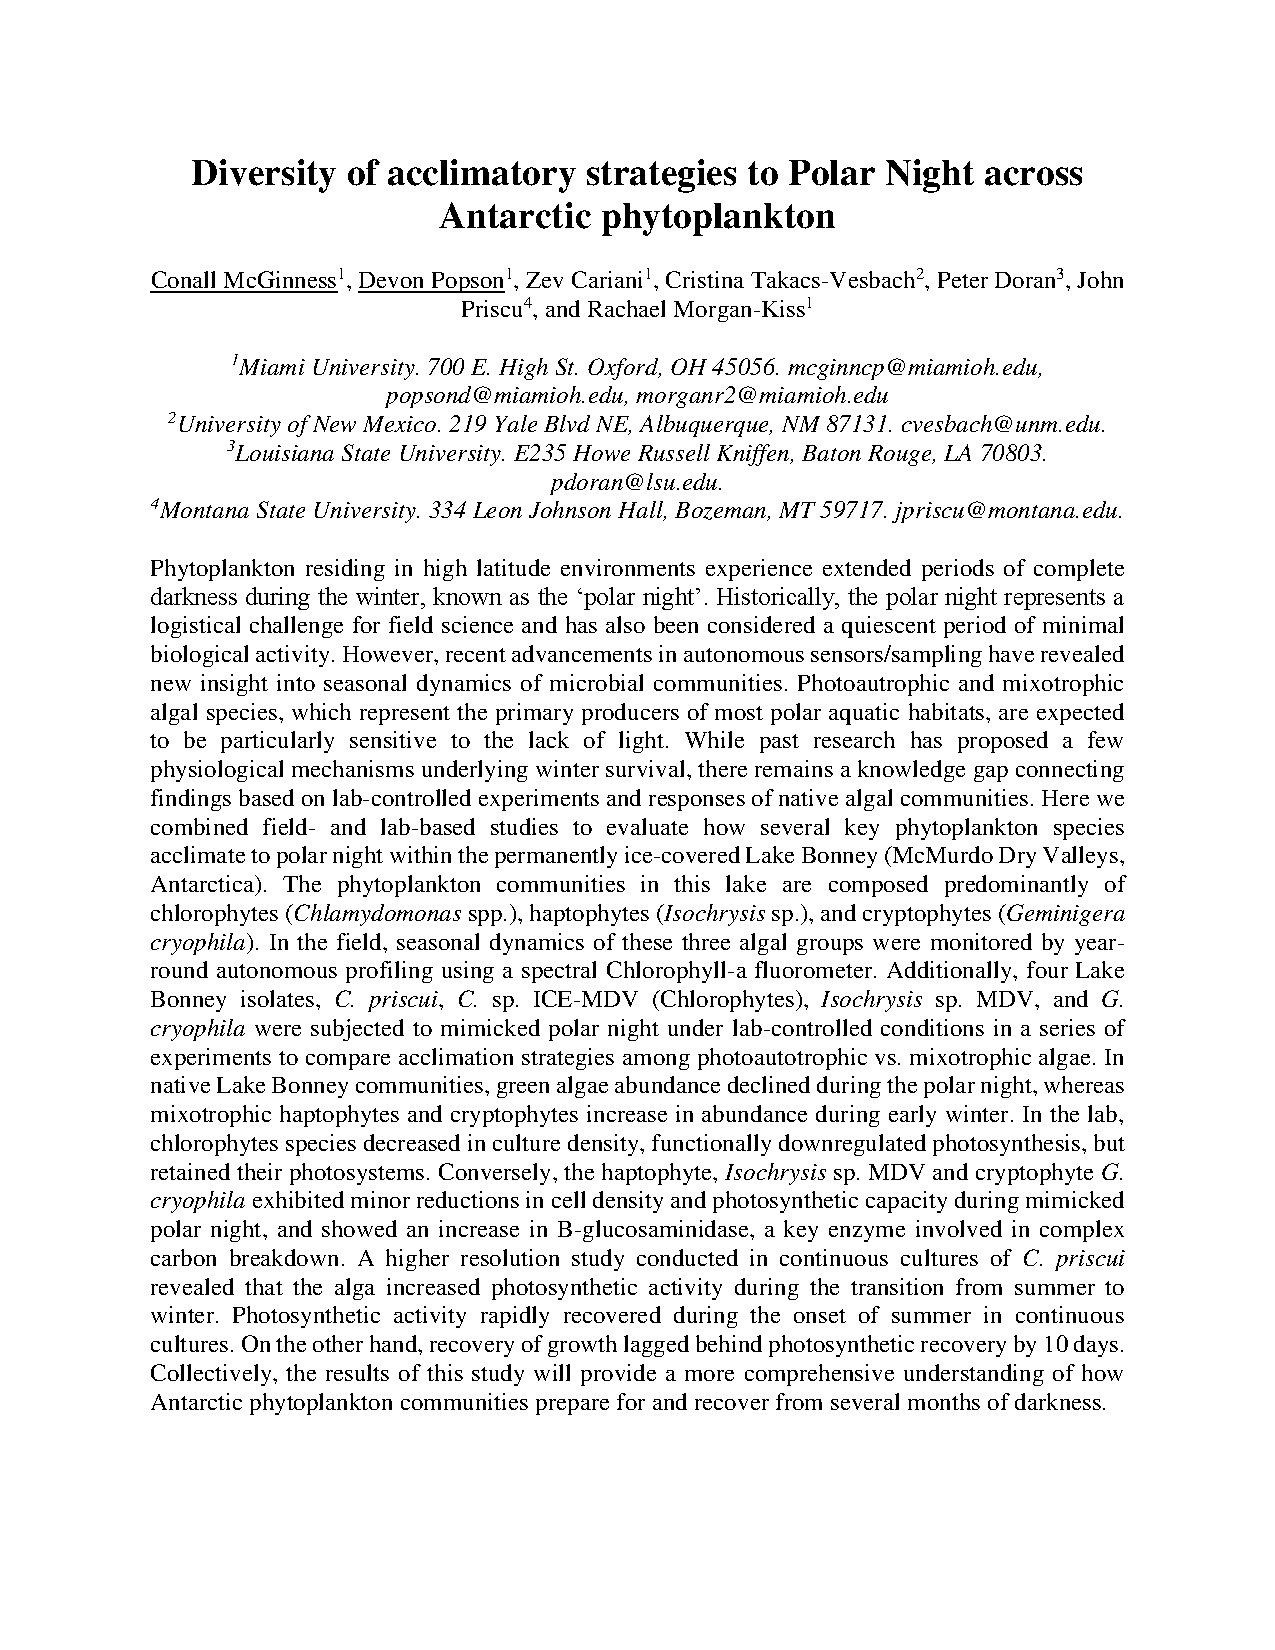
\includepdf[link=true,linkname=Mcginness,pagecommand={\thispagestyle{plain}},addtolist={1,nottalk,heading,abs:Mcginness}]{abstracts/McGinness_Popson_MWSE50.pdf}
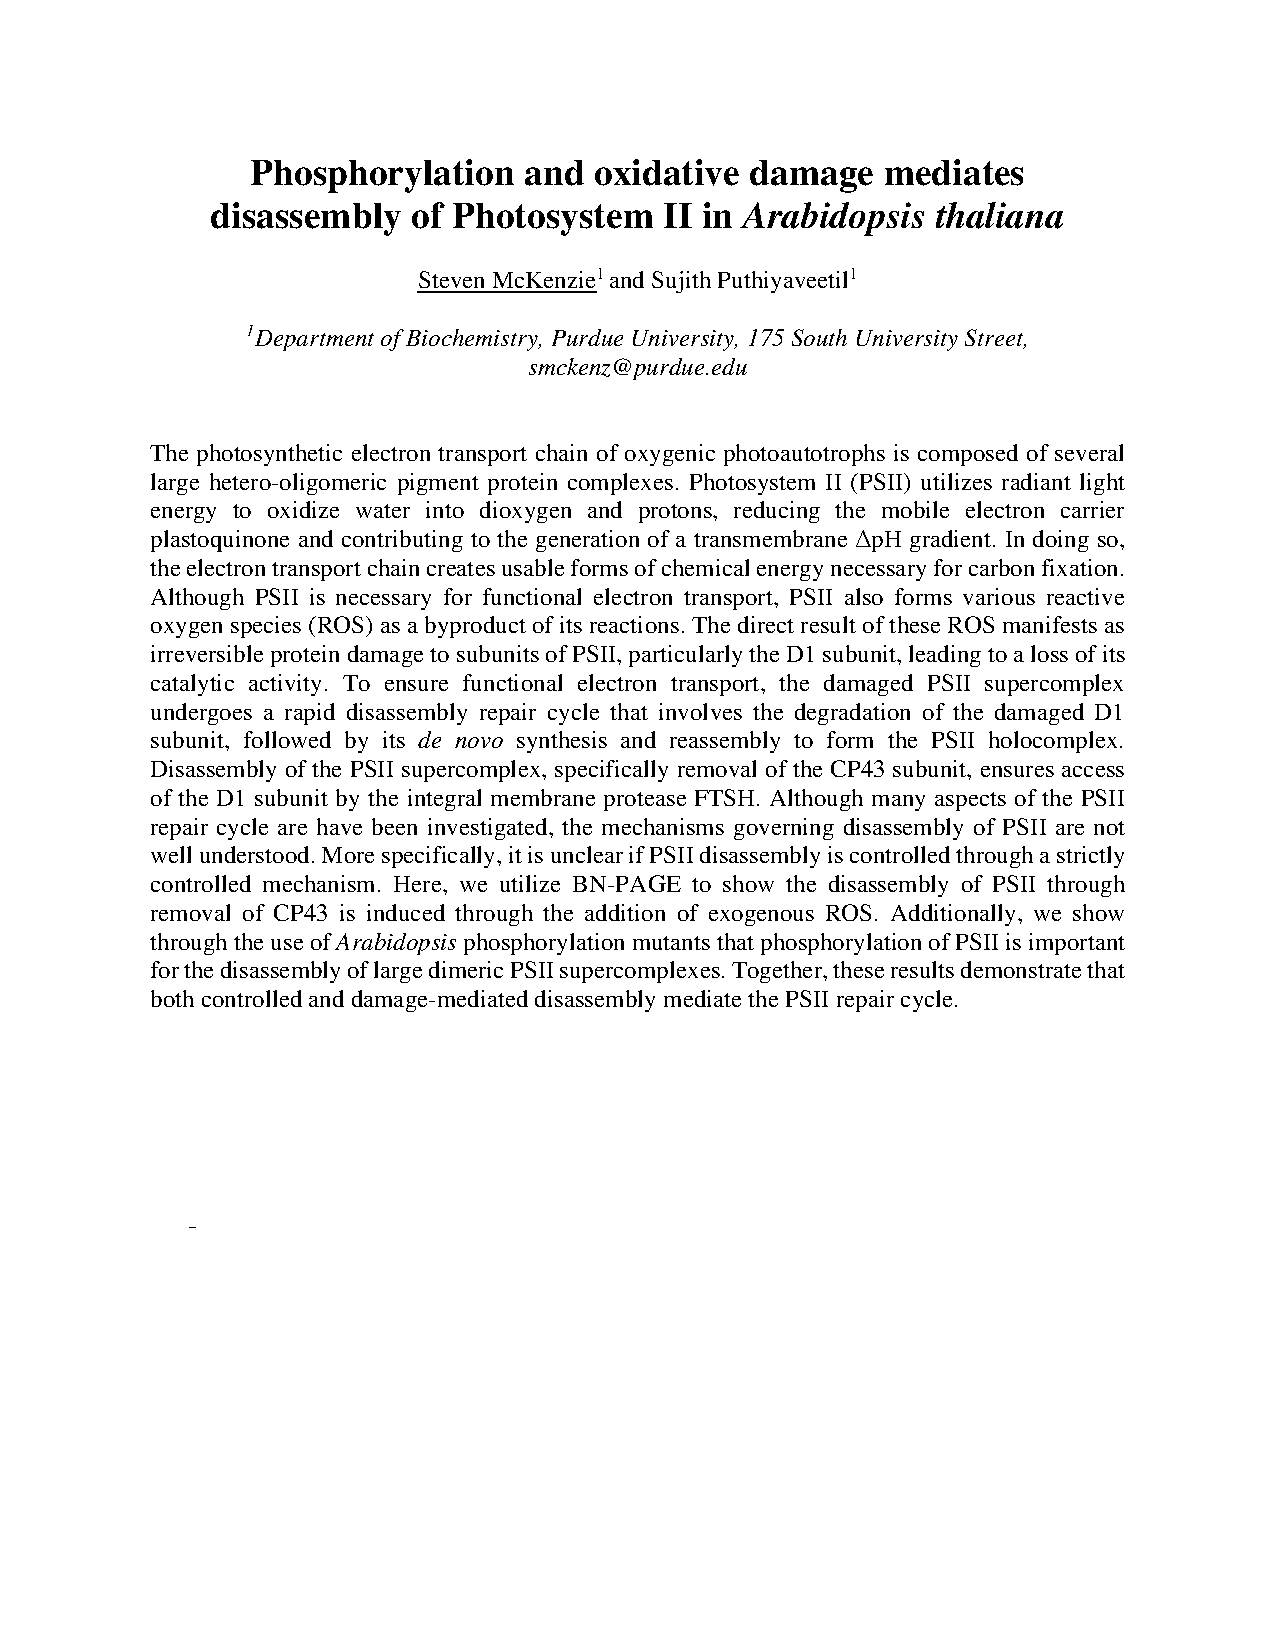
\includepdf[link=true,linkname=Mckenzie,pagecommand={\thispagestyle{plain}},addtolist={1,nottalk,heading,abs:Mckenzie}]{abstracts/McKenzie_MWSE50.pdf}
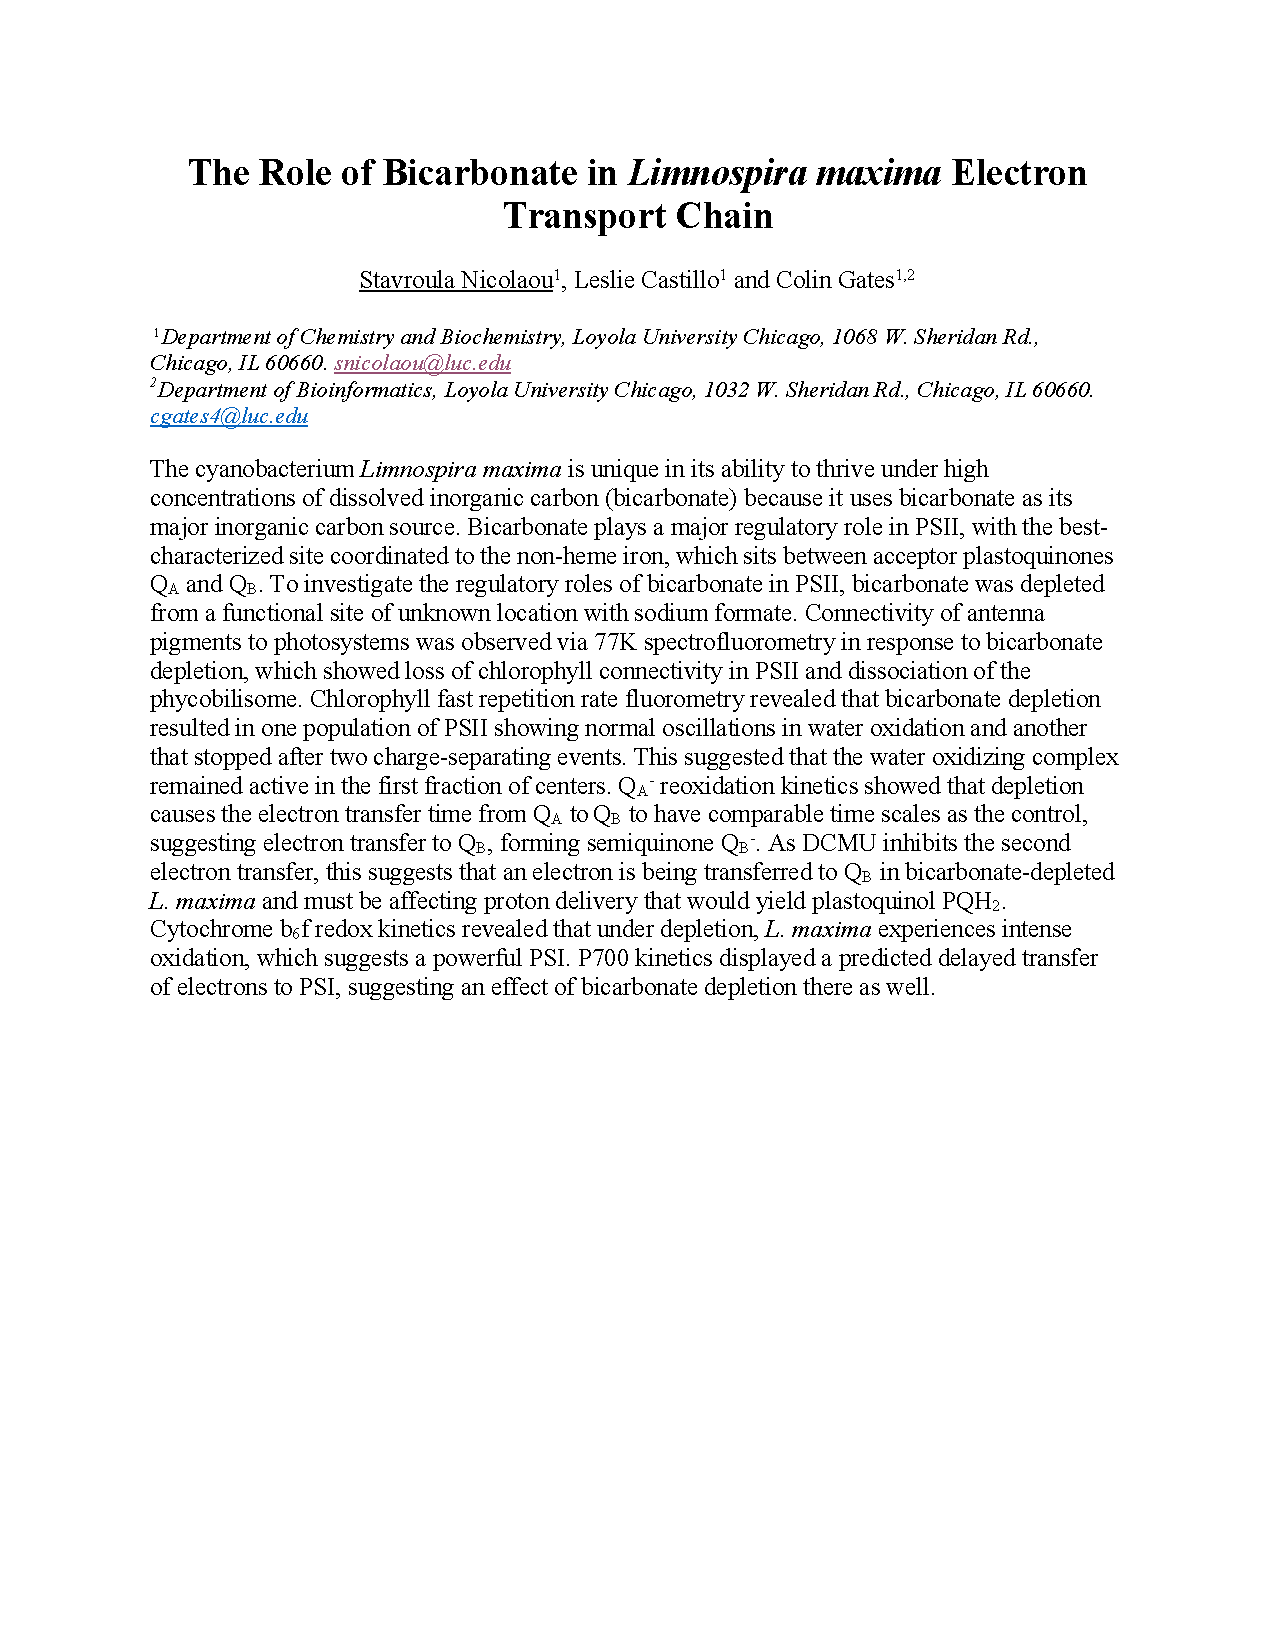
\includepdf[link=true,linkname=Nicolaou,pagecommand={\thispagestyle{plain}},addtolist={1,nottalk,heading,abs:Nicolaou}]{abstracts/Nicolaou_MWSE50.pdf}
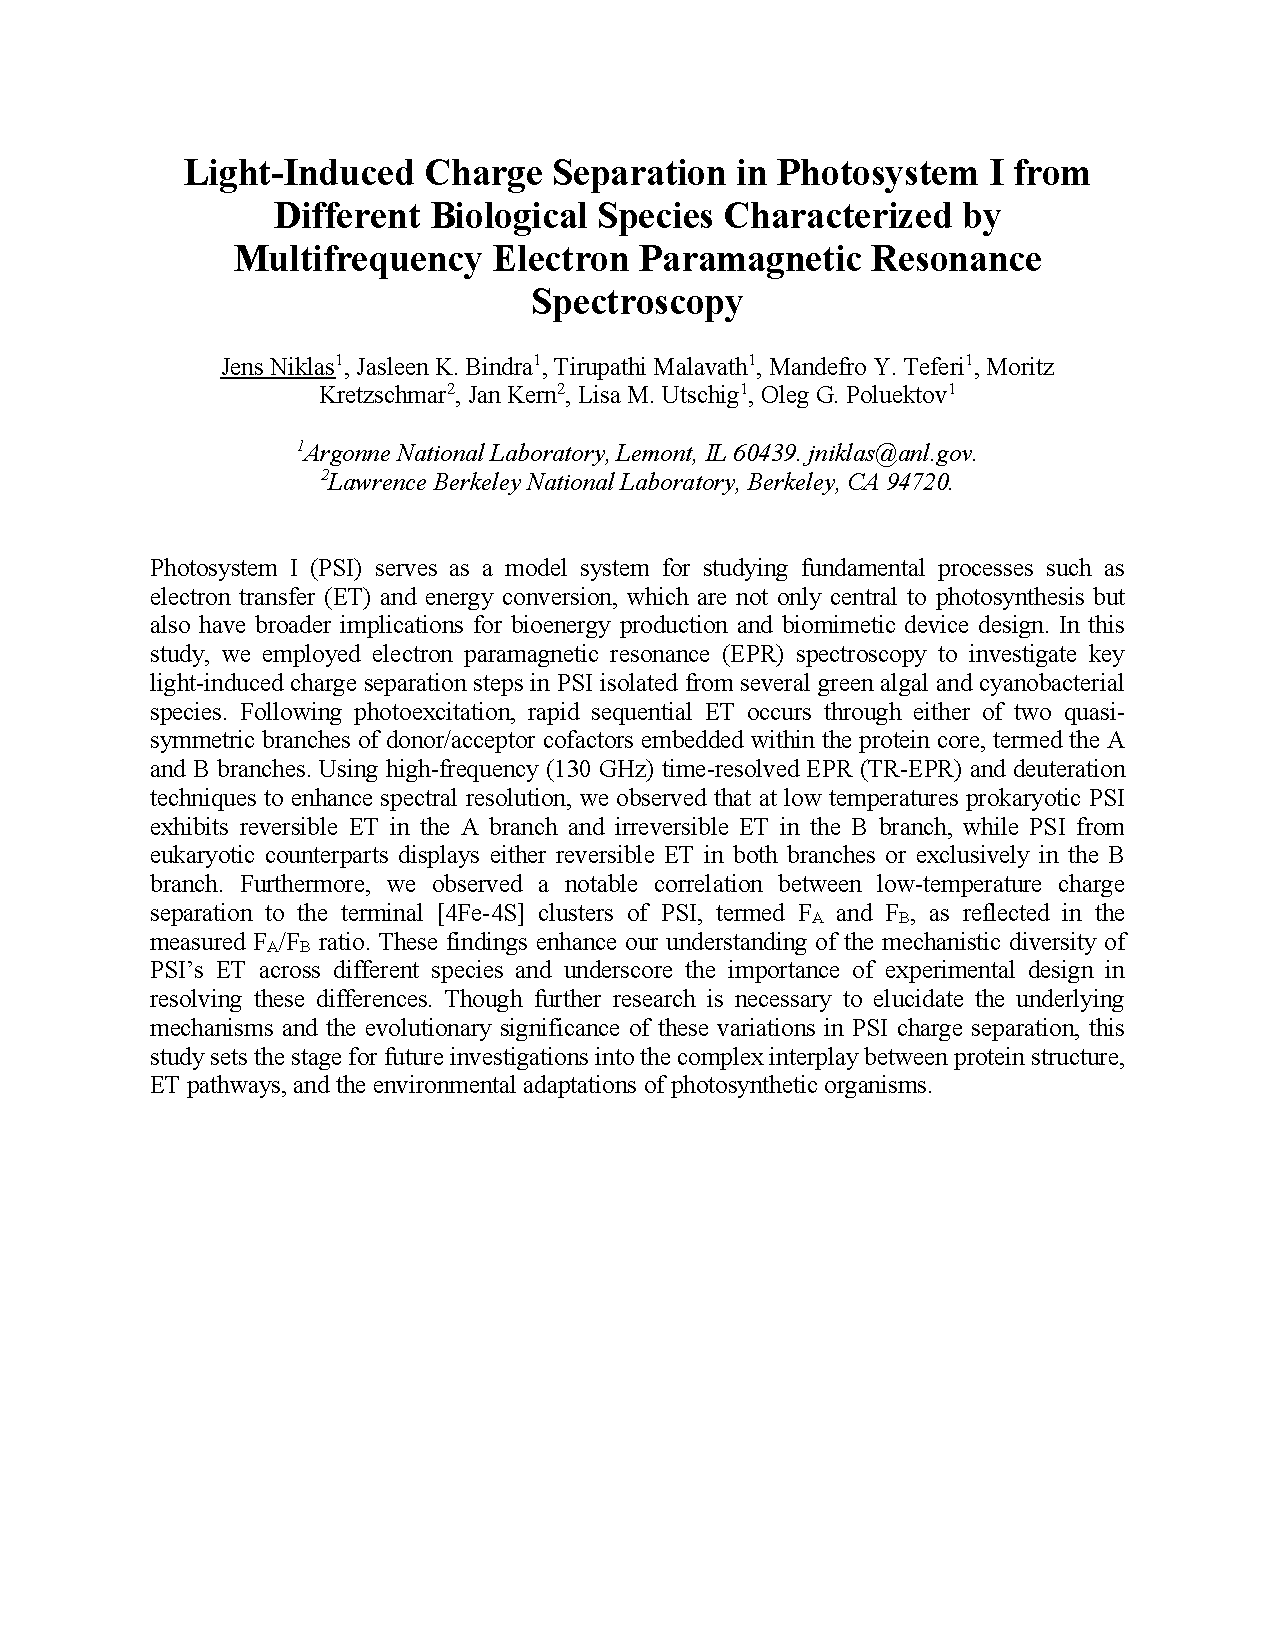
\includepdf[link=true,linkname=Niklas,pagecommand={\thispagestyle{plain}},addtolist={1,nottalk,heading,abs:Niklas}]{abstracts/Niklas_MWSE50.pdf}
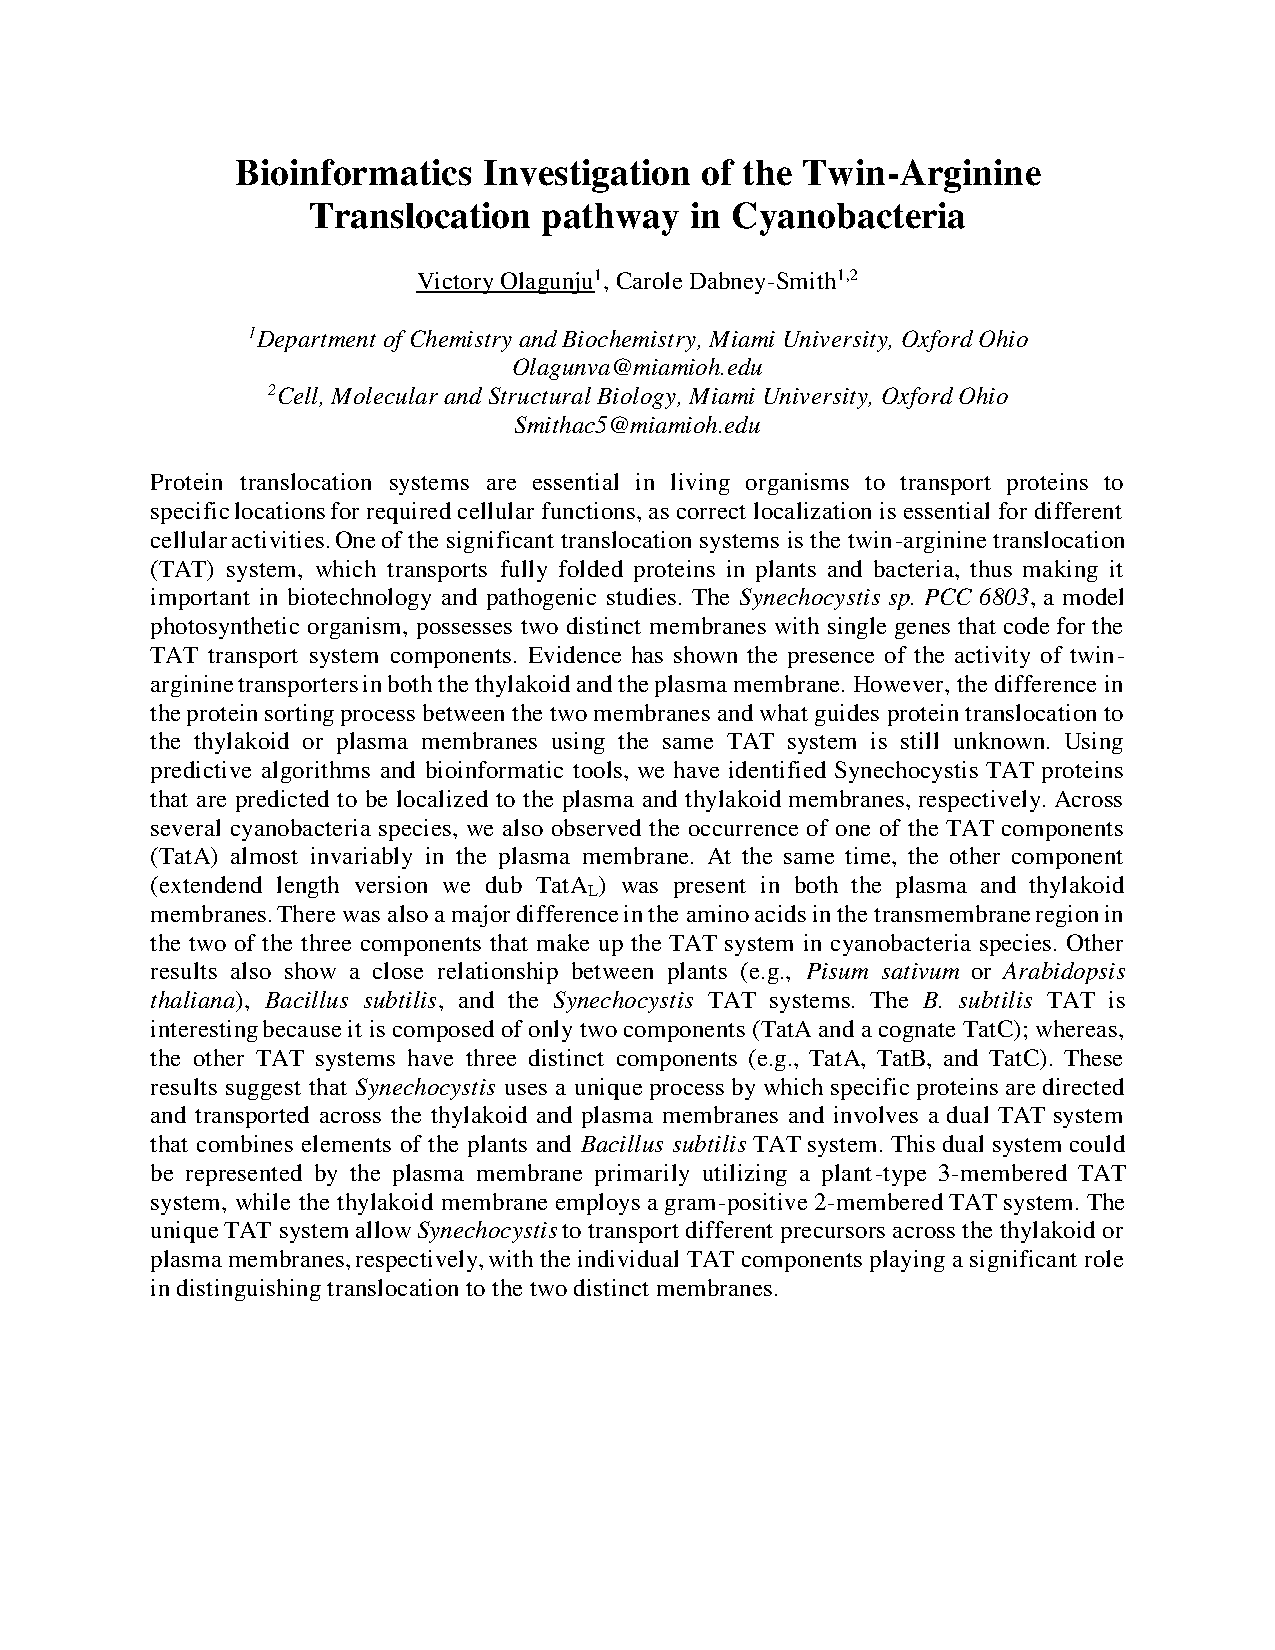
\includepdf[link=true,linkname=Olagunju,pagecommand={\thispagestyle{plain}},addtolist={1,nottalk,heading,abs:Olagunju}]{abstracts/Olagunju_MWSE50.pdf}
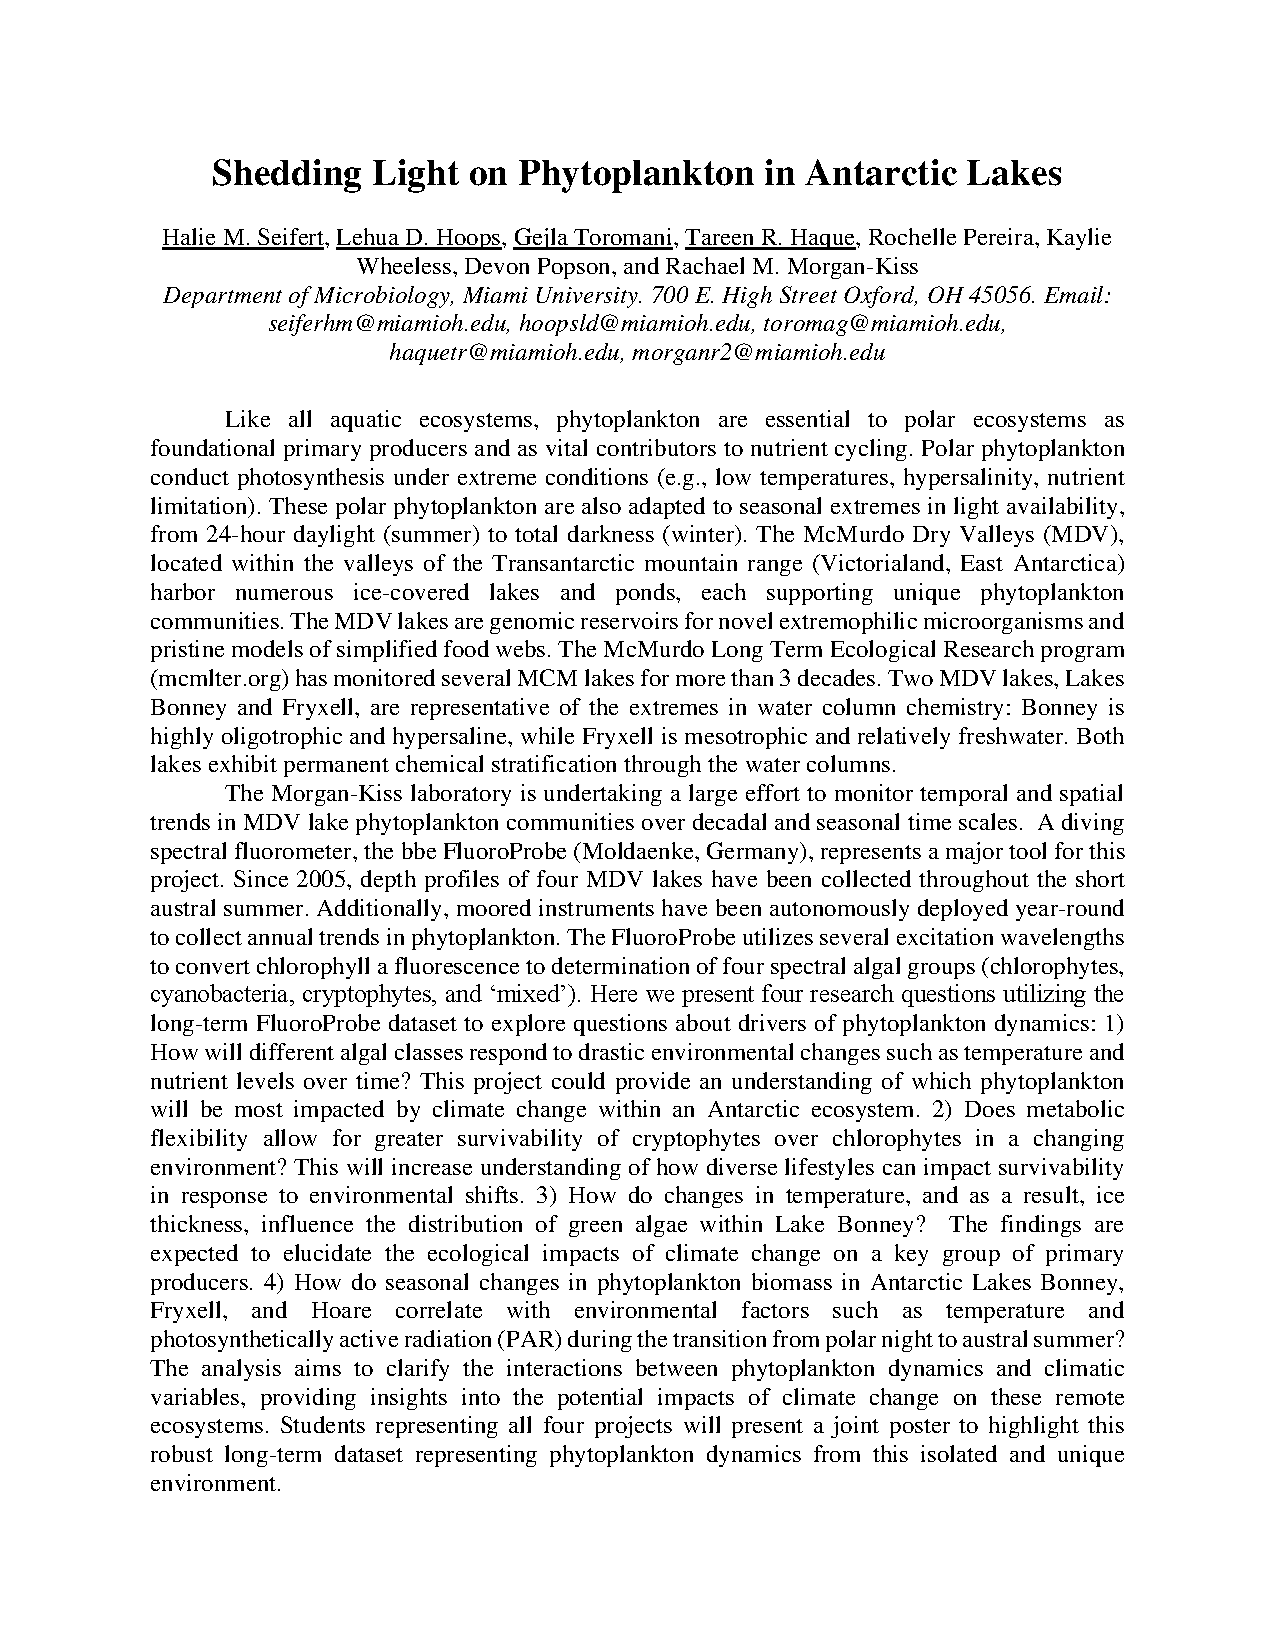
\includepdf[link=true,linkname=Seifert,pagecommand={\thispagestyle{plain}},addtolist={1,nottalk,heading,abs:Seifert}]{abstracts/Seifert_Hoops_Toromani_Haque_MWSE50.pdf}
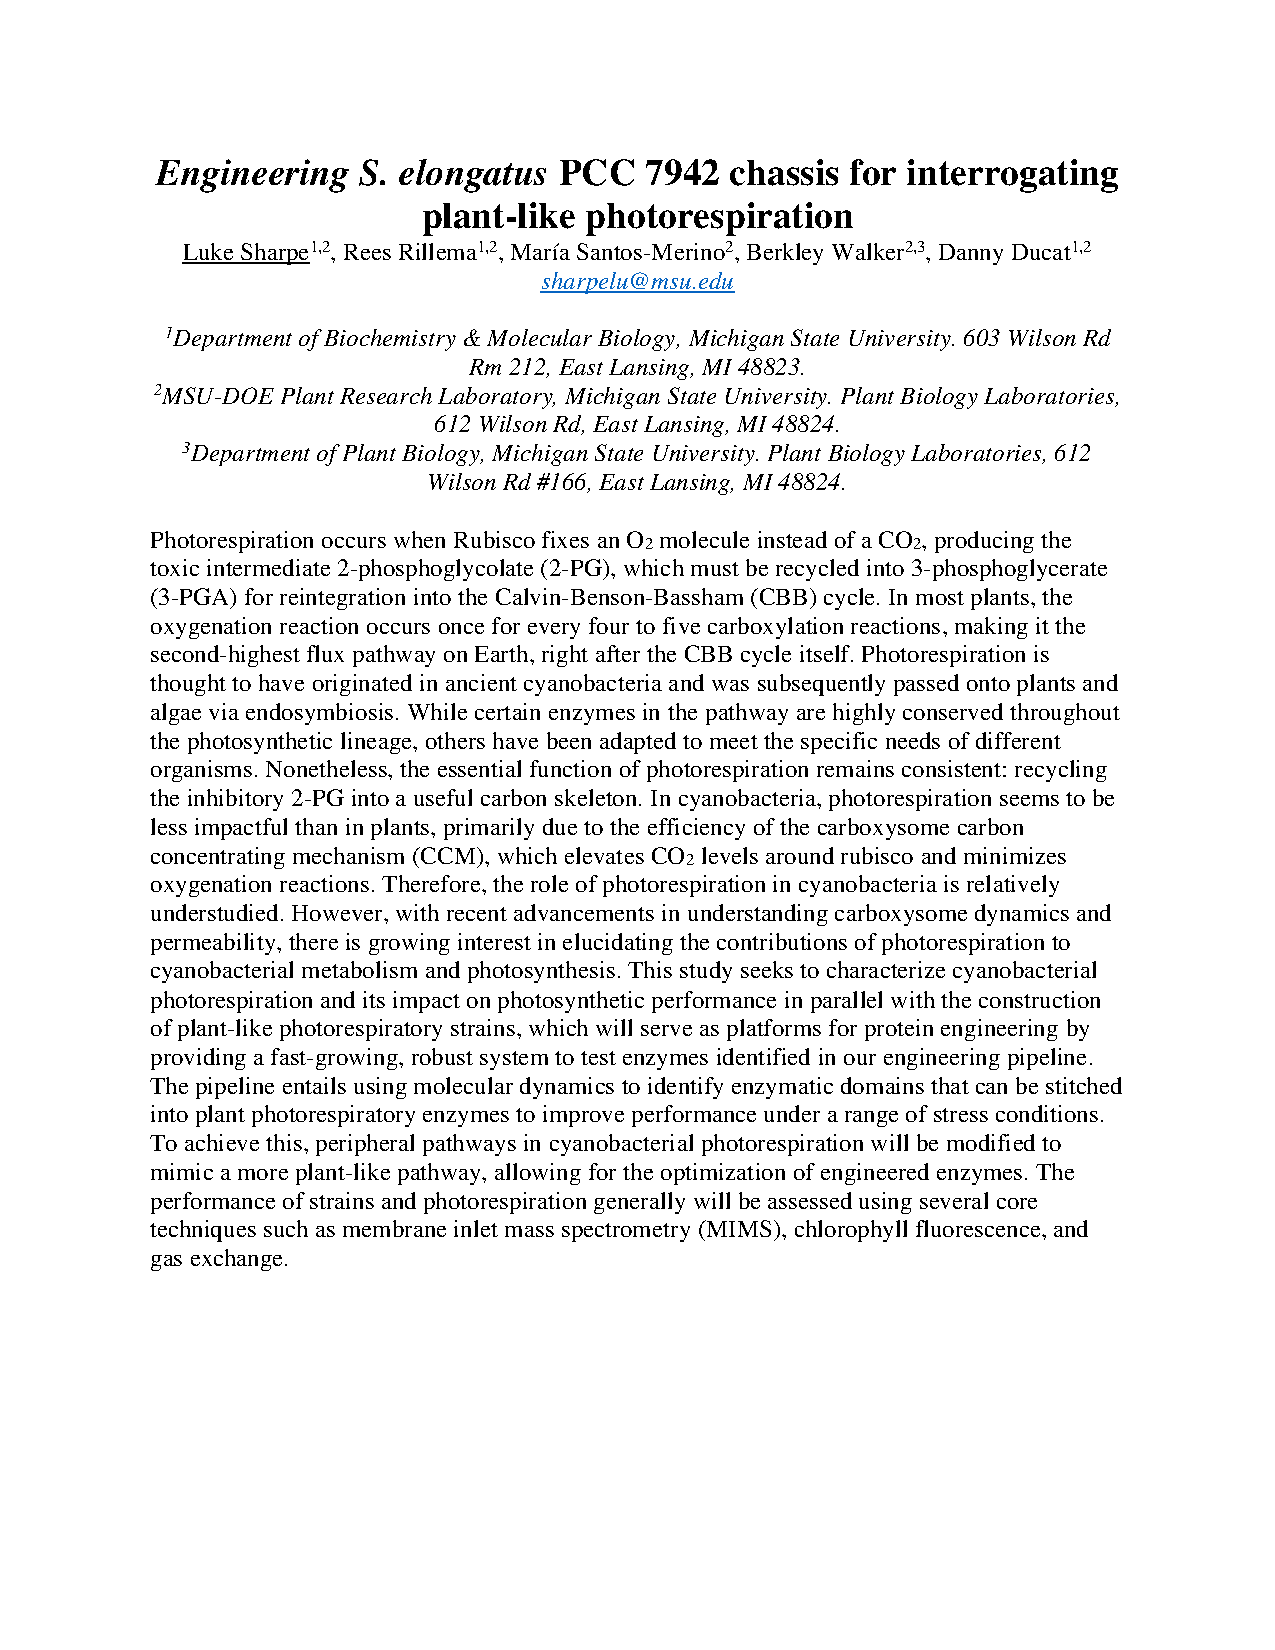
\includepdf[link=true,linkname=Sharpe,pagecommand={\thispagestyle{plain}},addtolist={1,nottalk,heading,abs:Sharpe}]{abstracts/Sharpe_MWSE50.pdf}
\includepdf[link=true,linkname=Short,pagecommand={\thispagestyle{plain}},addtolist={1,nottalk,heading,abs:Short}]{abstracts/Short_MWSE50_final.pdf}
\includepdf[link=true,linkname=Smolen,pagecommand={\thispagestyle{plain}},addtolist={1,nottalk,heading,abs:Smolen}]{abstracts/Smolen_MWSE50.pdf}
\includepdf[link=true,linkname=Snyder,pagecommand={\thispagestyle{plain}},addtolist={1,nottalk,heading,abs:Snyder}]{abstracts/Snyder_MWSE50.pdf}
\includepdf[link=true,linkname=Strong,pagecommand={\thispagestyle{plain}},addtolist={1,nottalk,heading,abs:Strong}]{abstracts/Strong_MWSE50.pdf}
\includepdf[link=true,linkname=Trembath,pagecommand={\thispagestyle{plain}},addtolist={1,nottalk,heading,abs:Trembath}]{abstracts/Trembath_MWSE50.pdf}
\includepdf[link=true,linkname=Tuncer,pagecommand={\thispagestyle{plain}},addtolist={1,nottalk,heading,abs:Tuncer}]{abstracts/Tuncer_MWSE50.pdf}
\includepdf[link=true,linkname=Weesinghe,pagecommand={\thispagestyle{plain}},addtolist={1,nottalk,heading,abs:Weesinghe}]{abstracts/Weesinghe_MWSE50.pdf}
\includepdf[link=true,linkname=Wheeless,pagecommand={\thispagestyle{plain}},addtolist={1,nottalk,heading,abs:Wheeless}]{abstracts/Wheeless_MWSE50.pdf}
\includepdf[link=true,linkname=Williams,pagecommand={\thispagestyle{plain}},addtolist={1,nottalk,heading,abs:Williams}]{abstracts/Williams_MWSE50.pdf}
\includepdf[link=true,linkname=Yadav,pagecommand={\thispagestyle{plain}},addtolist={1,nottalk,heading,abs:Yadav}]{abstracts/Yadav_MWSE50.pdf}

 
%----------------------------------------------------------------------------------------
%	 USEFUL INFORMATION
%----------------------------------------------------------------------------------------


\chapter{Useful Information}

The conference will be held at the Turkey Run Inn, just inside Turkey Run State Park in Marshall, Indiana October 25-27.
\textbf{Meals} will be in the main dining area, near the check-in desk. 
\textbf{Talks, coffee breaks, and posters} will be in the lower level, past the cozy lobby and down the stairs in the meeting area.
Forwarned is forarmed, the Wi-Fi can be spotty at Turkey Run, so please be prepared with flash drives to transfer presentations as needed.

\section{Organizing committee}

\begin{center}
	\begin{tabular}{ll}
		Sujith Puthiyaveetil (chair)	&		Josh Vermaas (co-chair) \\
		Department of Biochemistry		&	Plant Research Laboratory \\
		Purdue University		&			Department of Biochemistry	\\
		West Lafayette, IN	47907	&			Michigan State University \\
		spveetil@purdue.edu       		&	vermaasj@msu.edu\\
		
	\end{tabular}
\end{center}

\section{Participant List}

\begin{multicols}{2}
	\begin{enumerate}
\item Richmond	Arhin,	Purdue University
\item Anindita	Banerjee,	Washington University in Saint Louis
\item Kishan	Bharwad,	Loyola University Chicago
\item Sudip	Bhowmick,	Purdue University
\item Jasleen	Bindra,	Argonne National Laboratory
\item Sandeep	Biswas,	Washington University in St Louis
\item Duncan 	Boren,	Michigan State University
\item Chris	Brininger,	University of Wisconsin-Madison
\item Robert	Burnap,	Oklahoma State University
\item Leslie 	Castillo,	Loyola University Chicago
\item Claire	Chang,	Argonne National Laboratory
\item William	Cramer,	Purdue University
\item Carole	Dabney-Smith,	Miami University
\item Anica	Dadwal,	Saint Louis University
\item Lydia	Davies-Balogun,	Alabama State University 
\item Danny	Ducat,	Michigan State University
\item Madhushree	Dutta,	Purdue University 
\item Mohamed	Elrefaiy,	University of Texas at Austin
\item Nicholas	Ferrari,	Louisiana State University
\item Colin	Gates,	Loyola University Chicago
\item Christopher	Gisriel,	University of Wisconsin-Madison
\item Vishnupriya	Gokul, Raj	Saint Louis University
\item Govindjee	Govindjee,	University of Illinois Urbana-Champaign
\item Vidya	Gundlapalli,	Loyola University Chicago
\item Tareen	Haque,	Miami University
\item Maxwell	Harman,	Michigan State University
\item Laura	Hiotaky,	Purdue University
\item Savannah	Holt,	Purdue University 
\item Lehua	Hoops,	Miami University
\item Harvey	Hou,	Alabama State University
\item Jianping	Hu,	Michigan State University
\item Xiaotong	Jiang,	Michigan State University
\item Christopher	Jones,	Washington University in Saint Louis
\item Nimarsha	Kamaradiwela Arachchige,	Miami University
\item Arivu 	Kapoor,	Loyola University Chicago
\item Rajnandani	Kashyap,	Saint Louis University
\item Nidhi	Kulkarni, 	Louisiana State University 
\item K. V.	Lakshmi,	Rensselaer Polytechnic Institute
\item Karen	Liao,	Alabama State University
\item Michelle	Liberton,	Washington University in Saint Louis
\item Matt	Lima,	Washington University in St. Louis
\item Alizée	Malnoë,	Indiana University Bloomington
\item Matt	Martin,	Purdue University
\item Conall	McGinness,	Miami University 
\item Steven	McKenzie,	Purdue University
\item Himanshu 	Mehra,	University of Wisconsin-Madison
\item Lauren  Ann	Metskas,	Purdue University
\item Ashraf	Mohamed,	University of Texas at Austin
\item Rachael 	Morgan-Kiss,	Miami University
\item Stavroula 	Nicolaou,	Loyola University Chicago 
\item Dariusz	Niedzwiedzki,	Washington University in St Louis
\item Jens	Niklas,	Argonne National Laboratory
\item Victory	Olagunju,	Miami University
\item Himadri	Pakrasi,	Washington University in Saint Louis
\item Amala	Phadkule,	Purdue University
\item Nina	Ponomarenko,	Argonne National Laboratory
\item Devon	Popson,	Miami University
\item Sujith	Puthiyaveetil,	Purdue University 
\item Doran	Raccah,	University of Texas at Austin
\item Mike	Reppert,	Purdue University
\item Rees	Rillema,	Michigan State University 
\item Halie	Seifert,	Miami University
\item Chetna 	Sharma,	University of Florida
\item Luke	Sharpe,	Michigan State University
\item Audrey	Short,	Argonne National Laboratory
\item Alexandra	Siemer,	Rose-Hulman Institute of Technology
\item Evan	Smolen,	Loyola University Chicago
\item Samuel	Snyder,	Argonne National Laboratory
\item Chloe	Starkey,	University of Texas at Austin
\item Grant	Steiner,	Loyola University Chicago
\item Andrew	Strong,	Michigan State University
\item Mitchell	Ticoras,	Michigan State University
\item Gejla	Toromani,	Miami University
\item Blake	Trembath,	Saint Louis University
\item Hasan	Tuncer,	Purdue University
\item Lisa	Utschig,	Argonne National Laboratory
\item Michael	Vaughn,	SpectroLogix
\item Josh	Vermaas,	Michigan State University
\item Wim	Vermaas,	Arizona State University
\item David	Vinyard,	Louisiana State University
\item Vidusha	Weesinghe,	Miami University
\item Kaylie 	Wheeless,	Miami University
\item Alexandria	Wilcox,	Washington University in Saint Louis
\item Anna	Williams,	Saint Louis University 
\item Neetu	Yadav,	Michigan State University
	\end{enumerate}
\end{multicols}

\section{Code of Conduct}

The Midwest/Southeast Photosynthesis Conference is committed to providing a welcoming, inclusive, and harassment-free environment in all interactions regardless of race, age, ethnicity, national origin, language, gender, gender identity, sexual orientation, disability, physical appearance, political views, military service, health status or religion. We welcome the opportunity to bring photosynthesis research to all people regardless of their identity or background.

As a program that aims to share ideas and freedom of thought and expression, it is essential that the interaction between participants take place in an environment that recognizes the inherent worth of every person by being respectful of all. All participants strive to be empathetic, respectful, welcoming, friendly, and patient. We strive to be collaborative and use language that reflects our values.

The conference does not tolerate harassment in any form. Harassment is any form of behavior intended to exclude, intimidate or cause discomfort. Harassment includes, but is not limited to, the use of abusive or degrading language, intimidation, stalking, harassing photography or recording, inappropriate physical contact, and unwelcome sexual attention.

\subsection{Examples of unacceptable behavior}
All participants are committed to making participation in this community a harassment-free experience.

We will not accept harassment or other exclusionary behaviors or actions that are illegal, such as:

\begin{itemize}
	\item The use of sexualized language or imagery
	\item Excessive profanity (please avoid curse words; people differ greatly in their sensitivity to swearing)
	\item Posting sexually explicit or violent material
	\item Violent or intimidating threats or language directed against another person or group
	\item Inappropriate physical contact and/or unwelcome sexual attention or sexual comments
	\item Sexist, racist, or otherwise discriminatory jokes and language
	\item Trolling or insulting and derogatory comments
	\item Written or verbal comments which have the effect of excluding people on the basis of membership in a specific group, including level of experience, gender, gender identity and expression, sexual orientation, disability, neurotype, personal appearance, body size, race, ethnicity, age, religion, or nationality
	\item Public or private harassment
	\item Continuing to initiate interaction (such as photography, recording, messaging, or conversation) with someone after being asked to stop
	\item Sustained disruption of talks, events, or communications, such as heckling of a speaker
	\item Publishing (or threatening to post) other people’s personally identifying information (“doxing”), such as physical or electronic addresses, without explicit permission
	\item Other unethical or unprofessional conduct
	\item Advocating for, or encouraging, any of the above behaviors All participants are governed by local laws, including Turkey Run State Park rules and their organization’s code of conduct and policies.
\end{itemize}



\subsection{How to Submit a Report}
If you feel your safety is in jeopardy or the situation is an emergency, contact local law enforcement before making a report to the conference organizers. (In the U.S., dial 911.)

Anyone who experiences, observes or has knowledge of threatening behavior is expected to immediately report the incident to a member of the event organizing committee, state park staff, or a trusted friend or colleague. The Midwest/Southeast photosynthesis conference reserves the right to take appropriate action.

Take care of each other. Alert the organizers if you notice a dangerous situation, someone in distress, or violations of this code of conduct, even if they seem inconsequential. For possibly unintentional breaches of the code of conduct, you may want to respond to the person and point out this code of conduct (either in public or in private, whatever is most appropriate). If you would prefer not to do that, please report the issue to the conference chair or co-chair.

\subsubsection{What Happens Next}
All complaints will be reviewed and investigated and will result in a response that is deemed necessary and appropriate to the circumstances. All reports will be kept confidential, with the exception of cases where the organizers or state park staff determines the report should be shared with law enforcement. In those cases, the report will be shared with the proper legal authorities.

In some cases the conference organizers may determine that a public statement will need to be made. If that’s the case, the identities of all involved parties and reporters will remain confidential unless those individuals instruct us otherwise.

%----------------------------------------------------------------------------------------
%	 CLOSING PAGE
%----------------------------------------------------------------------------------------

\newpage

\thispagestyle{empty} % Suppress headers and footers on this page
\pagecolor{myblue} % Coloured background
~

%----------------------------------------------------------------------------------------

\end{document}
